\documentclass[12pt]{report}
\usepackage[utf8]{inputenc}
\usepackage{geometry}
\geometry{letterpaper, margin=0.25in}
\usepackage{graphicx} 
\usepackage{parskip}
\usepackage{booktabs}
\usepackage{array} 
\usepackage{paralist} 
\usepackage{verbatim}
\usepackage{subfig}
\usepackage{fancyhdr}
\usepackage{multirow}
\usepackage{sectsty}
\usepackage[shortlabels]{enumitem}

\pagestyle{fancy}
\renewcommand{\headrulewidth}{0pt} 
\lhead{}\chead{}\rhead{}
\lfoot{}\cfoot{\thepage}\rfoot{}

%%% ToC (table of contents) APPEARANCE
\usepackage[nottoc,notlof,notlot]{tocbibind} 
\usepackage[titles,subfigure]{tocloft}
\renewcommand{\cftsecfont}{\rmfamily\mdseries\upshape}
\renewcommand{\cftsecpagefont}{\rmfamily\mdseries\upshape} %

\usepackage{amsmath}
\usepackage{amssymb}
\usepackage{mathtools}
\usepackage{empheq}
\usepackage{xcolor}
\usepackage{bbm}
\usepackage{tikz}
\usepackage{pgfplots}
\usepackage{tikz-cd}
\pgfplotsset{compat=1.18}
\usetikzlibrary{intersections, calc, decorations.markings}
\usepgfplotslibrary{polar}
\usepgfplotslibrary{fillbetween}

\tikzset{
    marking along/.style n args={2}{
        decoration={
                markings, 
                mark=at position #1 with {\arrow{#2}}
        },
        postaction={decorate}
        },
    marking along/.default={0.5}{>},
    wavy/.style={
        decorate,decoration={coil,aspect=0}
    }, 
    two marks/.style n args={1}{
        decoration={
            markings,
            mark=at position 0.25 with {\arrow{#1}},
            mark=at position 0.75 with {\arrow{#1}}
        }
        postaction={decorate}

    },
    two marks/.default={>},
}

\usetikzlibrary{external}
\tikzexternalize
\tikzsetexternalprefix{figures/}
\tikzset{external/up to date check={md5}}

\newcommand{\ans}[1]{\boxed{\text{#1}}}
\newcommand{\vecs}[1]{\langle #1\rangle}
\renewcommand{\hat}[1]{\widehat{#1}}

\renewcommand{\P}{\mathbb{P}}
\newcommand{\R}{\mathbb{R}}
\newcommand{\E}{\mathbb{E}}
\newcommand{\Z}{\mathbb{Z}}
\newcommand{\N}{\mathbb{N}}
\newcommand{\Q}{\mathbb{Q}}
\newcommand{\C}{\mathbb{C}}

\newcommand{\ind}{\mathbbm{1}}
\newcommand{\qed}{\quad \blacksquare}

\newcommand{\brak}[1]{\left\langle #1 \right\rangle}
\newcommand{\bra}[1]{\left\langle #1 \right\vert}
\newcommand{\ket}[1]{\left\vert #1 \right\rangle}

\newcommand{\abs}[1]{\left\vert #1 \right\vert}
\newcommand{\mfX}{\mathfrak{X}}
\newcommand{\ep}{\varepsilon}

\newcommand{\Ec}{\mathcal{E}}
\newcommand{\A}{\mathcal{A}}
\newcommand{\F}{\mathcal{F}}
\newcommand{\Cc}{\mathcal{C}}
\newcommand{\B}{\mathcal{B}}
\newcommand{\M}{\mathcal{M}}
\newcommand{\X}{\chi}
\renewcommand{\L}{\mathcal{L}}

\newcommand{\sub}{\subseteq}
\newcommand{\st}{\text{ s.t. }}
\newcommand{\card}{\text{card }}
\renewcommand{\div}{\vspace*{10pt}\hrule\vspace*{10pt}}
\newcommand{\surj}{\twoheadrightarrow}
\newcommand{\inj}{\hookrightarrow}
\newcommand{\biject}{\hookrightarrow \hspace{-8pt} \rightarrow}
\renewcommand{\bar}[1]{\overline{#1}}
\newcommand{\overcirc}[1]{\overset{\circ}{#1}}
\newcommand{\diam}{\text{diam }}
\newcommand{\tr}{\text{tr}\,}
\renewcommand{\mod}{\text{mod}\,}

\renewcommand{\Re}{\text{Re}\,}
\renewcommand{\Im}{\text{Im}\,}
\newcommand{\sign}{\text{sign}\,}

\newcommand*{\tbf}[1]{\ifmmode\mathbf{#1}\else\textbf{#1}\fi}

\usepackage{tcolorbox}
\tcbuselibrary{breakable, skins}
\tcbset{enhanced}
\tcbset{shield externalize}

\newenvironment{tbox}[2][gray]{
    \begin{tcolorbox}[
        parbox=false,
        colback=#1!5!white,
        colframe=#1!75!black,
        breakable,
        title={#2}
    ]}
    {\end{tcolorbox}}

\newenvironment{exercise}[1][red]{
    \begin{tcolorbox}[
        parbox=false,
        colback=#1!5!white,
        colframe=#1!75!black,
        breakable
    ]}
    {\end{tcolorbox}}

\newenvironment{proof}[1][blue]{
\begin{tcolorbox}[
    parbox=false,
    colback=#1!5!white,
    colframe=#1!75!black,
    breakable
]}
{\end{tcolorbox}}

\newenvironment{proposition}[1][gray]{
\begin{tcolorbox}[
    parbox=false,
    colback=#1!5!white,
    colframe=#1!75!black,
    breakable
]}
{\end{tcolorbox}}

\colorlet{mygreen}{green!50!teal}

\title{APMA 1360: Applied Dynamical Systems}
\author{Milan Capoor}
\date{Spring 2025}

\begin{document}
\maketitle

\chapter{Bifurcation Theory}
\section{Jan 22}
\subsection*{Motivations - Applications + Phenomena}
\begin{enumerate}
    \item \tbf{Bifurcation theory:} How do systems change as parameters change?

          \emph{Examples:}
          \begin{itemize}
              \item Mechanical systems (e.g. what will happen to a bead as an apparatus is rotated at velocity $\omega$?)
              \item Chemical reactions (e.g. Belusov-Zhabotinsky reaction - oscillations in chemical reactions)
              \item Tipping points (e.g. climate change, convection currents)
              \item Population dynamics (e.g. predator-prey models, outbreaks)
              \item Synchronization (e.g. firefly synchronous lighting, brain activity patterns)
              \item Chaotic dynamics (e.g. double pendulum)
          \end{itemize}

    \item \tbf{Existence and Uniqueness}

    \item \tbf{Dynamical theory}

    \item \tbf{Chaotic dynamics}
\end{enumerate}

\subsection*{Bifurcation Theory}
\tbf{Example (Overdamped bead on loop)}

\begin{center}
    \begin{tikzpicture}
        \draw (0,0) circle (2);

        \node (B) at ({-sqrt(2)},{-sqrt(2)}) {};
        \draw[fill, blue] (B) circle (0.1);

        \draw[dashed, blue] (0,0) -- (B) node[midway, left] {$r$};

        \draw (0, 3) -- (0, -3);
        \draw[->, mygreen] (0, -1) arc (-90:-130:1) node[midway, below] {$\phi$};

        \draw[->, dashed, red, rotate=-90] ([shift=(-150:0.5)]-2, 0) arc (-150:150:0.1 and 0.5);

    \end{tikzpicture}
\end{center}

\tbf{Goal:} What will happen to the bead as the loop is rotated at velocity $\omega$?

We assume that the only forces on the bead are gravitation, friction, and centrifugal force.

This gives a force diagram:
\begin{center}
    \begin{tikzpicture}

        \draw (0,0) circle (0.05);
        \draw[->] (0, 0) -- (0,-2) node[below] {$mg$};

        \draw (0, 0) arc[start angle =-45, end angle = 0, radius = 2];
        \draw (0, 0) arc[start angle =-45, end angle = -90, radius = 2];

        \draw[->, dashed] (-2,0) -- (0,0);
        \draw[->] (0, 0) -- (2, 0) node[right] {$mr\omega^2\sin \phi$};

        \draw[blue] (-2, -2) -- (2, 2) node[above, right] {Tangent to loop};

        \draw[mygreen] (0.5, 0)  arc[start angle = 0, end angle = 45, radius = 0.5] node[right] {$\phi$};
    \end{tikzpicture}
\end{center}

From Newton's law,
\[\underbrace{mr \frac{d^2\phi}{dt^2}}_{\text{acceleration}} = -b \frac{d\phi}{dt} - mg \sin \phi + m\omega^2 r \sin\phi \cos \phi\]

Assuming $b \gg 1$, we can neglect the LHS so
\begin{align*}
    \frac{d\phi}{dt} & = -\frac{mg}{b}\sin \phi + \frac{m\omega^2 r}{b} \sin \phi \cos \phi    \\
                     & = \frac{mg}{b} \sin \phi \left(\frac{\omega^2 r}{g} \cos \phi- 1\right) \\
                     & = a \sin \phi (\mu \cos \phi - 1)
\end{align*}

\section{Jan 24}
\subsection*{Review}
\tbf{Definition:} A function $u(t)$ is a solution of $\dot u = f(u)$ if $\frac{du(t)}{dt} = f(u(t))$ for all $t$ in some open interval. In this case, we say ``$u(t)$ satisfies $\dot u = f(u)$''.

\begin{tbox}{\textbf{Theorem (Existence and Uniqueness):} Assume $f \in C^1$ (class of continuously differentiable functions) and $u_0 \in \R$ is given. Then the differential equation $\dot u = f(u)$ with initial condition $u(0) = u_0$ has a unique solution $u(t)$ on some open interval containing $t = 0$.}
    \emph{Proof:} Omitted
\end{tbox}

\tbf{Example:} $\dot u = au, u(0) = u_0$ has solution $u(t) = u_0 e^{at}$. Since $au$ is continuous, $u(t) \in C^1$, hence the solution is unique.

\subsection*{Geometric Viewpoint}

\tbf{Example:} Consider $\dot u = f(u)$,
\begin{center}
    \begin{tikzpicture}
        \begin{axis}[
                axis lines=middle,
                no markers,
                enlargelimits,
                xtick=\empty,
                ytick=\empty,
                axis line style={->},
                xlabel style={at={(current axis.right of origin)}, anchor=west},
                ylabel style={at={(current axis.above origin)}, anchor=south},
                domain=-6:6,
                samples=20
            ]
            \addplot[blue, thick] {-(x+5)*(2*x+3)*(x-5)};

            \node[red, above] (u1) at (axis cs:-5,-0.6) {$u_1$};
            \node[red, above] (u2) at (axis cs:-3/2,0) {$u_2$};
            \node[red, right, above] (u3) at (axis cs:5,0) {$u_3$};

            \node[red] at (axis cs:-5,0) {$\bullet$};
            \node[red] at (axis cs:-3/2,0) {$\bullet$};
            \node[red] at (axis cs:5,0) {$\bullet$};
        \end{axis}
    \end{tikzpicture}
\end{center}

For each point, $f(u_i) = 0 \implies u(t) = u_i$ is a solution for all $t$.

We can check:
\[\begin{cases}
        \frac{du}{dt}(t) = \frac{d}{dt} u_i = 0 \\
        f(u(t)) = f(u_i) = 0
    \end{cases}\]
Hence, $u(t) = u_i$ is a solution.

We call the points $u_1, u_2, u_3$ \emph{equilibrium points}, \emph{rest states}, \emph{steady states}, \emph{fixed points}, or \emph{stationary points}.

We can also consider the direction field of $\dot u = f(u(t))$:
\[\begin{cases}
        f(u) < 0 \implies u \text{ decreasing} \implies u \text{ moves left} \\
        f(u) > 0 \implies u \text{ increasing} \implies u \text{ moves right}
    \end{cases}\]

So we can draw the phase diagram
\begin{center}
    \begin{tikzpicture}
        \begin{axis}[
                axis lines=middle,
                no markers,
                enlargelimits,
                xtick=\empty,
                ytick=\empty,
                axis line style={->},
                xlabel style={at={(current axis.right of origin)}, anchor=west},
                ylabel style={at={(current axis.above origin)}, anchor=south},
                domain=-6:6,
                samples=20
            ]
            \addplot[blue, thick] {-(x+5)*(2*x+3)*(x-5)};

            \node[red, above] (u1) at (axis cs:-5, 0) {$u_1$};
            \node[red, above] (u2) at (axis cs:-3/2,0) {$u_2$};
            \node[red, above] (u3) at (axis cs:5,0) {$u_3$};

            \coordinate (u1) at (axis cs:-5,0);
            \coordinate (u2) at (axis cs:-3/2,0);
            \coordinate (u3) at (axis cs:5,0);


            \node[mygreen] at (axis cs:-4.5, 0) {$<$};
            \node[mygreen] at (axis cs:-5.5, 0) {$>$};

            \node[mygreen] at (axis cs:-2, 0) {$<$};
            \node[mygreen] at (axis cs:-1, 0) {$>$};

            \node[mygreen] at (axis cs:4.5, 0) {$>$};
            \node[mygreen] at (axis cs:5.5, 0) {$<$};
        \end{axis}
        \draw[red, fill] (u1) circle (0.05);
        \draw[red, fill] (u2) circle (0.05);
        \draw[red, fill] (u3) circle (0.05);


    \end{tikzpicture}
\end{center}

In this case, we say that $u_1, u_3$ are stable but $u_2$ is unstable.

\tbf{Stable:} an equilibrium $u_i$ is stable if all solutions for initial conditions near $u_i$ converge to $u_i$ as $t \to \infty$.

\tbf{Unstable:} an equilibrium $u_i$ is unstable if there exists an initial condition near (but distinct from) $u_i$ such that the solution moves away from $u_i$ as $t \to \infty$.

\tbf{Conditions for stability:} Assuming $u_i$ is an equilibrium,
\begin{itemize}
    \item If $f'(u_i) < 0$, then $u_i$ is stable.
    \item If $f'(u_i) > 0$, then $u_i$ is unstable.
    \item If $f'(u_i) = 0$, then it is undetermined
\end{itemize}

What can $f'(u_i) = 0$ look like?

\emph{Examples:}

\begin{center}
    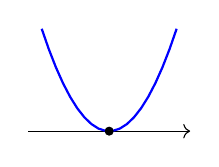
\begin{tikzpicture}
        \begin{axis}[
                width=0.3\textwidth,
                axis lines=middle,
                no markers,
                enlargelimits,
                xtick=\empty,
                ytick=\empty,
                axis line style={->},
                domain=-2:2,
                samples=20,
                hide y axis
            ]
            \addplot[blue, thick] {x^2};
            \coordinate (O) at (axis cs: 0, 0);
        \end{axis}
        \draw[fill] (O) circle (0.05);
    \end{tikzpicture}
    \hspace{1cm}
    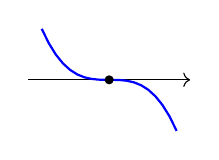
\begin{tikzpicture}
        \begin{axis}[
                width=0.3\textwidth,
                axis lines=middle,
                no markers,
                enlargelimits,
                xtick=\empty,
                ytick=\empty,
                axis line style={->},
                domain=-2:2,
                samples=20,
                hide y axis
            ]
            \addplot[blue, thick] {-x^3};
            \coordinate (O) at (axis cs: 0, 0);
        \end{axis}
        \draw[fill] (O) circle (0.05);

    \end{tikzpicture}
\end{center}

\subsection*{Example 1 Revisited:} Recall
\[\dot \phi = a \sin \phi(\mu \cos \phi - 1) = f(\phi)\]
for $a, \mu > 0$ and $\mu \approx \omega^2$.

\begin{enumerate}
    \item We can verify $f \in C^1$.

    \item Find the equilibrium points:
          \[a \sin \phi (\mu \cos \phi - 1) = 0 \implies \phi = \{0, \pi\}\]

    \item Determine stability:
          \begin{align*}
              f'(\phi) \bigg\vert_{\phi = 0, \pi} & = \left[a \cos \phi (\mu \cos \phi - 1)\right]_{\phi = 0, \pi} \\
                                                  & = \begin{cases}
                                                          a(\mu - 1) & \phi = 0   \\
                                                          a(\mu + 1) & \phi = \pi
                                                      \end{cases}
          \end{align*}

          Hence, $\phi = 0$ is always unstable since $a(\mu + 1) > 0$. $\phi = \pi$ is stable $\mu < 1$, unstable $\mu > 1$ and undetermined for $\mu = 1$.

          In fact, this makes sense. $\mu$ is the ratio of the centrifugal force to the gravitational force. If $\mu < 1$, the gravitational force is stronger and the bead will fall to the bottom. If $\mu > 1$, the centrifugal force is stronger and the bead will move outwards.

\end{enumerate}


\section{Jan 27}
\tbf{Recall:} We return one more time to the example of the bead on a loop. Last time, we determined the system has equilibria
\begin{center}
    %% Bead on loop equilibrium diagram
    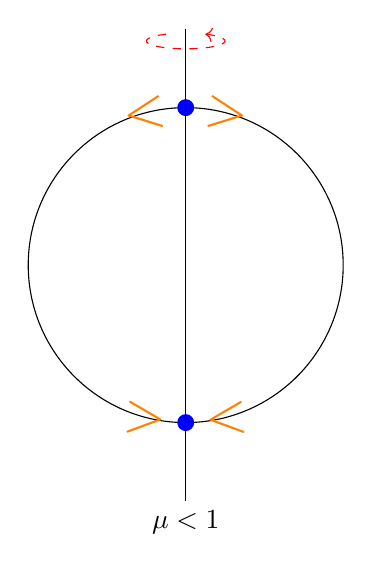
\begin{tikzpicture}
        \draw (0,0) circle (2);

        \node (top) at (0, 2) {};
        \node (bot) at (0, -2) {};
        \draw[fill, blue] (top) circle (0.1);
        \draw[fill, blue] (bot) circle (0.1);

        \node[scale=2, orange, rotate=-8] at (top) [right] {$>$};
        \node[scale=2, orange, rotate=8] at (top) [left] {$<$};

        \node[scale=2, orange, rotate=5] at (bot) [right] {$<$};
        \node[scale=2, orange, rotate=-5] at (bot) [left] {$>$};


        \draw (0, 3) -- (0, -3) node[below] {$\mu < 1$};

        \draw[->, dashed, red, rotate=-90] ([shift=(-150:0.5)]-2.5, 0) arc (-150:150:0.1 and 0.5);
    \end{tikzpicture}
    \hspace{1cm}
    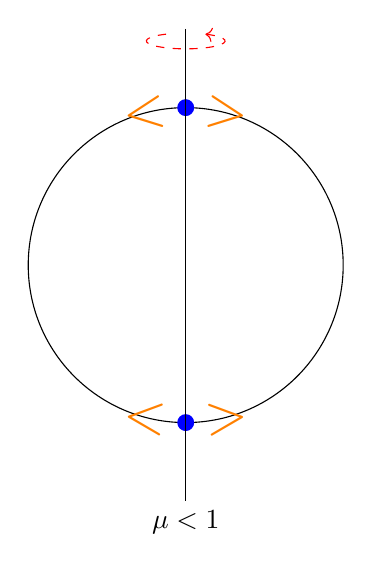
\begin{tikzpicture}
        \draw (0,0) circle (2);

        \node (top) at (0, 2) {};
        \node (bot) at (0, -2) {};
        \draw[fill, blue] (top) circle (0.1);
        \draw[fill, blue] (bot) circle (0.1);

        \node[scale=2, orange, rotate=-8] at (top) [right] {$>$};
        \node[scale=2, orange, rotate=8] at (top) [left] {$<$};

        \node[scale=2, orange, rotate=5] at (bot) [right] {$>$};
        \node[scale=2, orange, rotate=-5] at (bot) [left] {$<$};


        \draw (0, 3) -- (0, -3) node[below] {$\mu < 1$};

        \draw[->, dashed, red, rotate=-90] ([shift=(-150:0.5)]-2.5, 0) arc (-150:150:0.1 and 0.5);



    \end{tikzpicture}
\end{center}

In the case on the right, the equilibria are not consistent. Therefore, there need to be additional equilibria.

We can check:
\[f(\phi) - a \sin \phi (\mu \cos \phi - 1)\]

Setting $a \sin \phi = 0$ gives $\phi = \{0, \pi\}$. Taking $\mu \cos \phi - 1 = 0$ gives $\phi = \arccos \frac{1}{\mu}$:
\begin{center}
    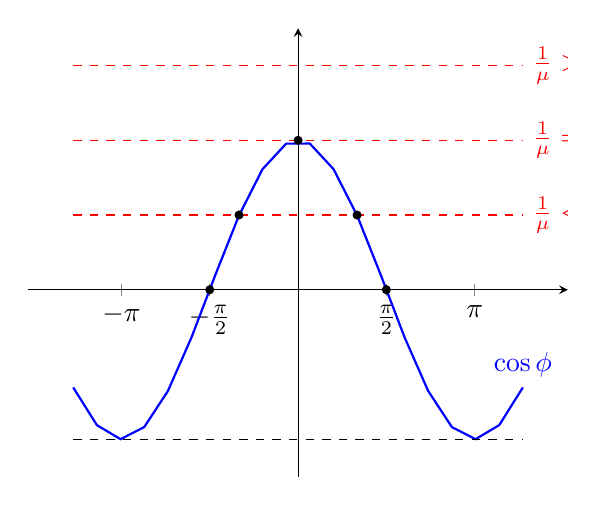
\begin{tikzpicture}
        \begin{axis}[
                axis lines=middle,
                no markers,
                enlargelimits,
                xtick={-pi, -pi/2, 0, pi/2, pi},
                ytick=\empty,
                xlabel=\empty,
                xticklabels={$-\pi$, $-\frac{\pi}{2}$, 0, $\frac{\pi}{2}$, $\pi$},
                domain=-4:4,
                samples=20
            ]
            \addplot[blue, thick] {cos(deg(x))};
            \addplot[red, dashed] {3/2} node[right] {$\frac{1}{\mu}> 1$};
            \addplot[red, dashed] {1} node[right] {$\frac{1}{\mu} = 1$};
            \addplot[red, dashed] {1/2} node[right] {$\frac{1}{\mu}< 1$};
            \addplot[dashed] {-1};


            \coordinate (A) at (axis cs: pi/2, 0);
            \coordinate (B) at (axis cs: -pi/2, 0);
            \coordinate (C) at (axis cs: 0, 1);
            \coordinate (D) at (axis cs: 1.05, 1/2);
            \coordinate (E) at (axis cs: -1.05, 1/2);

            \coordinate (lab) at (axis cs: 4, -0.5);


        \end{axis}
        \draw[fill] (A) circle (0.05);
        \draw[fill] (B) circle (0.05);
        \draw[fill] (C) circle (0.05);
        \draw[fill] (D) circle (0.05);
        \draw[fill] (E) circle (0.05);

        \node[blue] at (lab) {$\cos \phi$};



    \end{tikzpicture}
\end{center}

This gives us the bifurcation diagram:

\begin{center}
    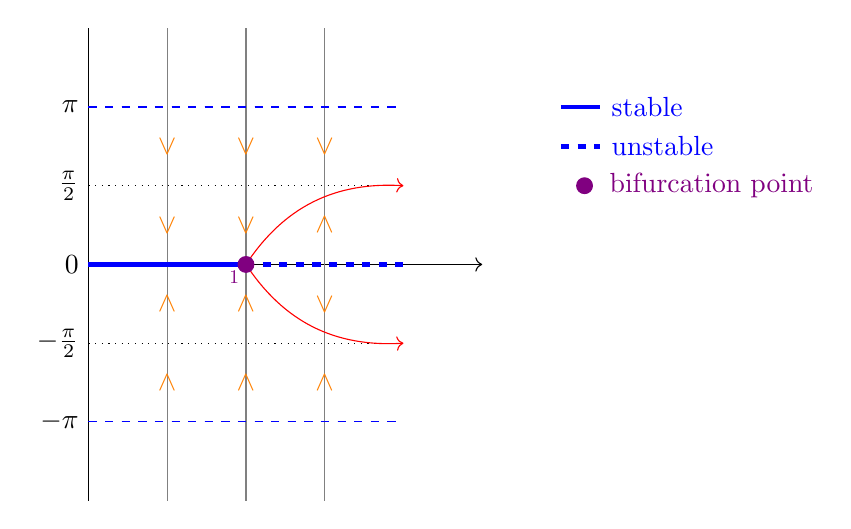
\begin{tikzpicture}
        \node[left] (O) at (0, 0) {$0$};
        \draw (0, -3) -- (0, 3); % y-axis
        \draw[->] (0, 0) -- (5, 0); % x-axis

        \node[left] (pi-y) at (0, 2) {$\pi$};
        \draw[dashed, blue] (pi-y) -- (4, 2);
        \node[left] (pi2-y) at (0, 1) {$\frac{\pi}{2}$};
        \draw[dotted] (pi2-y) -- (4, 1);

        \node[left] (mpi-y) at (0, -2) {$-\pi$};
        \draw[dashed, blue] (mpi-y) -- (4, -2);
        \node[left] (mpi2-y) at (0, -1) {$-\frac{\pi}{2}$};
        \draw[dotted] (mpi2-y) -- (4, -1);

        \draw[gray] (1, -3) -- (1, 3);
        \draw[gray] (2, -3) -- (2, 3);
        \draw[gray] (3, -3) -- (3, 3);

        \draw[blue, ultra thick] (0, 0) -- (2, 0);
        \draw[blue, ultra thick, dashed] (2, 0) -- (4, 0);
        \draw[blue, dashed] (0,2) -- (4, 2);
        \draw[blue, dashed] (0,-2) -- (4, -2);

        \node[orange] at (1, 1.5) {\rotatebox{180}{$\wedge$}};
        \node[orange] at (2, 1.5) {\rotatebox{180}{$\wedge$}};
        \node[orange] at (3, 1.5) {\rotatebox{180}{$\wedge$}};
        \node[orange] at (1, 0.5) {\rotatebox{180}{$\wedge$}};
        \node[orange] at (2, 0.5) {\rotatebox{180}{$\wedge$}};
        \node[orange] at (3, 0.5) {$\wedge$};

        \node[orange] at (1, -0.5) {$\wedge$};
        \node[orange] at (2, -0.5) {$\wedge$};
        \node[orange] at (3, -0.5) {\rotatebox{180}{$\wedge$}};
        \node[orange] at (1, -1.5) {$\wedge$};
        \node[orange] at (2, -1.5) {$\wedge$};
        \node[orange] at (3, -1.5) {$\wedge$};

        \draw[->, red] (2, 0) to[bend left] (4, 1);
        \draw[->, red] (2, 0) to[bend right] (4, -1);

        \draw[red!50!blue, fill] (2, 0) circle (0.1) node[scale=0.7, below left]{$1$};

        \draw[blue, ultra thick] (6, 2) -- (6.5, 2) node[right] {stable};
        \draw[blue, ultra thick, dashed] (6, 1.5) -- (6.5, 1.5) node[right] {unstable};
        \draw[red!50!blue, fill] (6.3, 1) circle (0.1) node[right]{\;\;bifurcation point};


    \end{tikzpicture}
\end{center}




where the curve is given by $\mu = \frac{r\omega^2}{g} \approx \frac{\text{centrifugal}}{\text{gravitational}}$.

Notice if $f'(\phi_*) \neq 0$, then the equilibrium $\phi_*$ varies continuously with $\mu$. If $f'(\phi_*) =0$, then new equilibria emerge and dynamics change.

\subsection*{Parameter-Dependent Differential Equations:} Consider $\dot u = f(u, \mu)$ for $u, \mu \in \R$ and $f: \R^2 \to \R$.

\tbf{Example:} $f(u, 0) = u$
%% $f(u, 0) = u$.
\begin{center}
    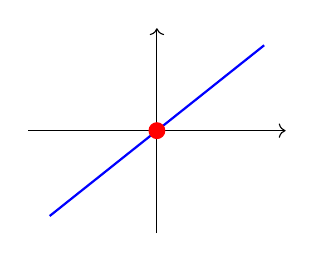
\begin{tikzpicture}
        \begin{axis}[
                width=0.4\textwidth,
                axis lines=middle,
                no markers,
                enlargelimits,
                xtick=\empty,
                ytick=\empty,
                axis line style={->},
                domain=-1:1,
                samples=20,
            ]
            \addplot[blue, thick] {x};
            \coordinate (O) at (axis cs: 0, 0);
        \end{axis}
        \draw[fill, red] (O) circle (0.1        );
    \end{tikzpicture}
\end{center}

Here, $u = 0$ is an unstable equilibrium. ($f(0, 0) =0$ and $f_u(0, 0) = 1 > 0$).

What happens if we change $\mu$ slightly? Choose $\mu \approx 0$:

\begin{center}
    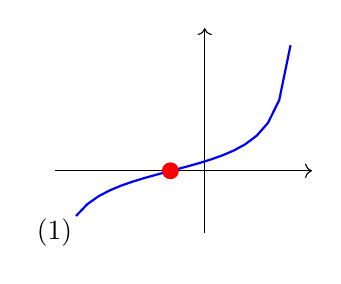
\begin{tikzpicture}
        \begin{axis}[
                width=0.4\textwidth,
                axis lines=middle,
                no markers,
                enlargelimits,
                xtick=\empty,
                ytick=\empty,
                axis line style={->},
                domain=-1.5:1,
                samples=20,
            ]
            \addplot[blue, thick] {tan(deg(x+pi/8))};
            \coordinate (O) at (axis cs: -0.4, 0);
        \end{axis}
        \draw[fill, red] (O) circle (0.1);
        \node (0, 0) {(1)};
    \end{tikzpicture}
    \hspace{1cm}
    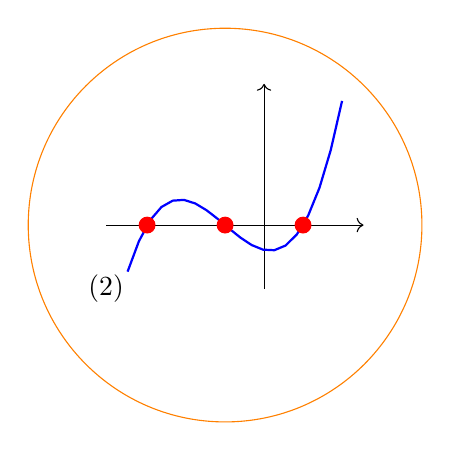
\begin{tikzpicture}
        \begin{axis}[
                width=0.4\textwidth,
                axis lines=middle,
                no markers,
                enlargelimits,
                xtick=\empty,
                ytick=\empty,
                axis line style={->},
                domain=-3.5:2,
                samples=20,
            ]
            \addplot[blue, thick] {(x+3)*(x+1)*(x-1)};
            \coordinate (A) at (axis cs: -3, 0);
            \coordinate (B) at (axis cs: -1, 0);
            \coordinate (C) at (axis cs: 1, 0);

            \coordinate (O) at (axis cs: -1, 0);

        \end{axis}
        \draw[fill, red] (A) circle (0.1);
        \draw[fill, red] (B) circle (0.1);
        \draw[fill, red] (C) circle (0.1);

        \draw[orange] (O) circle (2.5);


        \node (0, 0) {(2)};
    \end{tikzpicture}
\end{center}

On the left, the equilibrium moves but is unique and still unstable. On the right, we have three equilibria and we can shrink the ball as $\mu \to 0$.

For (2), say
\[f(u, \mu) = \begin{cases}
        u + \mu                            & u \leq -\mu          \\
        \frac{u}{2}(\frac{u^2}{\mu^2} - 1) & -\mu \leq u \leq \mu \\
        u - \mu                            & u = \mu
    \end{cases}\]
with $\abs{f(u, \mu)} \leq \text{const.}$ uniformly in $\mu, u$

\tbf{Properties of (2):}
\begin{itemize}
    \item $f(u, \mu)$ is continuous in $u, \mu$.
    \item $f(u, \mu)$ is differentiable in $u$ for all $(u, \mu)$
    \item $f_u(u, \mu)$ is not continuous
\end{itemize}

For simplicity, we will consider only functions $f(u, \mu)$ that are infinitely often differentiable and for which all derivatives are continuous in $(u, \mu)$, i.e. $f \in C^{\infty}(\R^2, \R) = C^{\infty}$

\tbf{Goal:} Assume $u_0$ is an equilibrium $\dot u = f(u, \mu)$ for $\mu = \mu_0$ so that when $f_u(u_0, \mu_0) \neq 0$, there is a function $g(\mu)$ so that $f(u, \mu) = 0$ for $(u, \mu)$ near $(u_0, \mu_0)$ iff $u = g(\mu)$.

\begin{center}
    \begin{tikzpicture}
        % Draw the axes
        \draw[->] (0,0) -- (5,0) node[right] {$\mu$};
        \draw[->] (0,0) -- (0,5) node[above] {$u$};

        % Draw the tick and label at the center
        \draw (0.2,2.5) -- (-0.3,2.5) node[left] {$u_0$};
        \draw (2.5,0.2) -- (2.5,-0.3) node[below] {$\mu_0$};
        \node[below right] at (2.5,2.5) {$(\mu_0, u_0)$};

        \draw[fill] (2.5, 2.5) circle (0.05);

        % Draw the curve
        \draw[blue, thick, domain=0:5, samples=20] plot (\x, {2.5 + 2.5*sin((\x-2.5)*180/5)}) node[right] {$\{(u, \mu): f(u, \mu) = 0\}$};

    \end{tikzpicture}
\end{center}

\begin{tbox}{\textbf{Implicit Function Theorem}: Assume $f(u_0, \mu_0) = 0$ and $f_u(u_0, \mu_0)\neq 0$ for $f \in C^{\infty}$. Then there exists open  intervals, $I, J$ with $u_0 \in J, \mu_0 \in I$ and a $g: I \to J$ such that $f(u, \mu) = 0$ for $(u, \mu) \in J \times I$ iff $u =g(\mu)$. Furthermore, $g \in C^{\infty}$. In particular, if $u_0$ is an equilibrium of $\dot u = f(u, \mu)$ at $\mu = \mu_0$ with $f_u(u_0, \mu_0) \neq 0$, then $\dot u = f(u, \mu)$ has an equilibrium in $J  \times I$ iff $u = g(\mu)$ and these equilibria share their stability properties with $u_0$}
    \emph{Example:}
    \begin{center}
        \begin{tikzpicture}
            % Draw the axes
            \draw[->] (0,0) -- (5,0) node[right] {$\mu$};
            \draw[->] (0,0) -- (0,5) node[above] {$u$};

            % Draw the tick and label at the center
            \draw (0.2,2.5) -- (-0.3,2.5) node[red, left] {$u_0$};
            \draw (2.5,0.2) -- (2.5,-0.3) node[red, below] {$\mu_0$};

            \draw[red, fill] (2.5, 2.5) circle (0.1);

            % Draw the curve
            \draw[blue, thick, domain=0:5, samples=20] plot (\x, {2.5 + 2.5*sin((\x-2.5)*180/5)}) node[right] {$u=g(\mu)$};

            \draw[orange!90!black, ultra thick] (2, 0) -- (3, 0) node[below right] {$I$};
            \draw[orange!90!black, ultra thick] (0, 2) -- (0, 3) node[above left] {$J$};

            \draw[orange, dashed, ultra thick] (2, 2) -- (3, 2) -- (3, 3) -- (2, 3) -- cycle;

        \end{tikzpicture}
    \end{center}
    \div
    \emph{Proof:} Omitted
\end{tbox}

\section{Jan 29}
\subsection{Implicit Function Theorem}re
\tbf{Recall:} If we have $f = f(u, \mu) \in C^{\infty}$ with $f(u_0, \mu_0) = 0$ and $f_u(u_0, \mu_0) \neq 0$, then there exist open intervals $I, J$ with $\mu_0 \in I$, $u_0 \in J$ and a unique $g: I \to J$ with $g(\mu_0) = u_0$ so that $f(u, \mu) = 0$ for $(u, \mu) \in J \times I$ iff $u = g(\mu)$. Furthermore, $g \in C^{\infty}$.

\begin{center}
    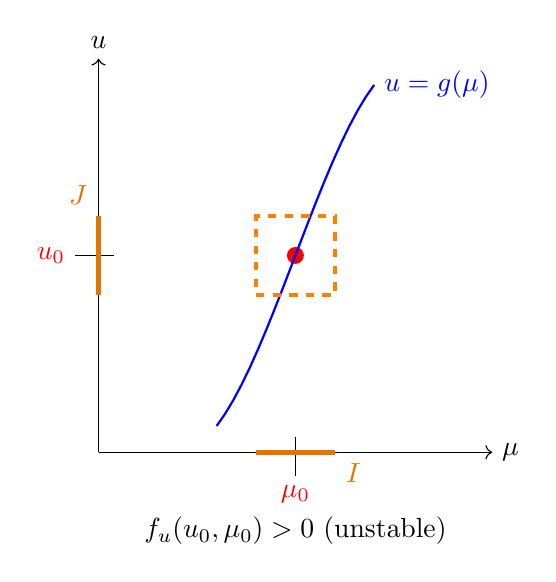
\begin{tikzpicture}
        % Draw the axes
        \draw[->] (0,0) -- (5,0) node[right] {$\mu$};
        \draw[->] (0,0) -- (0,5) node[above] {$u$};

        % Draw the tick and label at the center
        \draw (0.2,2.5) -- (-0.3,2.5) node[red, left] {$u_0$};
        \draw (2.5,0.2) -- (2.5,-0.3) node[red, below] {$\mu_0$};

        \draw[red, fill] (2.5, 2.5) circle (0.1);

        % Draw the curve
        \draw[blue, thick, domain=1.5:3.5, samples=20] plot (\x, {2.5 + 2.5*sin((\x-2.5)*180/3)}) node[right] {$u=g(\mu)$};

        \draw[orange!90!black, ultra thick] (2, 0) -- (3, 0) node[below right] {$I$};
        \draw[orange!90!black, ultra thick] (0, 2) -- (0, 3) node[above left] {$J$};

        \draw[orange, dashed, ultra thick] (2, 2) -- (3, 2) -- (3, 3) -- (2, 3) -- cycle;

        \node at (2.5, -1) {$f_u(u_0, \mu_0) > 0 \text{ (unstable)}$};
    \end{tikzpicture}
    \hspace{1cm}
    \begin{tikzpicture}
        % Draw the axes
        \draw[->] (0,0) -- (5,0) node[right] {$\mu$};
        \draw[->] (0,0) -- (0,5) node[above] {$u$};

        % Draw the tick and label at the center
        \draw (0.2,2.5) -- (-0.3,2.5) node[red, left] {$u_0$};
        \draw (2.5,0.2) -- (2.5,-0.3) node[red, below] {$\mu_0$};

        \draw[red, fill] (2.5, 2.5) circle (0.1);

        % Draw the curve
        \draw[blue, thick, domain=1.5:3.5, samples=20] plot (\x, {2.5 + (\x-2.5)^2}) node[right] {$u=g(\mu)$};

        \draw[orange!90!black, ultra thick] (2, 0) -- (3, 0) node[below right] {$I$};
        \draw[orange!90!black, ultra thick] (0, 2) -- (0, 3) node[above left] {$J$};

        \draw[orange, dashed, ultra thick] (2, 2) -- (3, 2) -- (3, 3) -- (2, 3) -- cycle;

        \node at (2.5, -1) {$f_u(u_0, \mu_0) < 0 \text{ (stable)}$};


    \end{tikzpicture}
\end{center}

\tbf{Definition:} we say that $u_0$ is a \tbf{hyperbolic equilibrium} of $\dot u = f(u, \mu)$ at $\mu = \mu_0$ if
\begin{itemize}
    \item $f(u_0, \mu_0) = 0$ ($u_0$ is an equilibrium)
    \item $f_u(u_0, \mu_0) \neq 0$ ($u_0$ is hyperbolic)
\end{itemize}

\emph{Example:} if $u_0$ is \emph{not} hyperbolic, the dynamics can be more complicated when we vary $\mu$ near $\mu_0$.

\begin{center}
    % Right Parabola
    \begin{tikzpicture}
        \draw (0, 0) -- (5, 0) node[right] {$\mu$};
        \draw (0, -2) -- (0, 2) node[above] {$u$};

        \coordinate (pt) at (2.5, 0);
        \begin{axis}[at=(pt), anchor=west, no markers, axis lines=middle, hide y axis, hide x axis]
            \addplot[blue] ({x^2}, x);
        \end{axis}

        \draw[red, ultra thick] (0, 0) -- (2.5, 0);
        \draw[red, ultra thick, dashed] (2.5, 0) -- (5, 0);

        \draw[red, fill] (2.5, 0) circle (0.1) node[below left] {$f_u(0, 1) = 0$};
    \end{tikzpicture}
\end{center}

Here the equilibrium on the red line is hyperbolic.

\tbf{Catalogue of Bifurcations:}
\begin{itemize}
    \item Consider $\dot u = f(u, \mu)$ with $u, \mu \in \R$ and $f \in C^{\infty}$.
    \item Assume WLOG that $(u, \mu) = (0, 0)$ is an equilibrium with
          \[\begin{cases}
                  f(0, 0) = 0 \\
                  f_u(0, 0) = 0
              \end{cases}\]
          (i.e. $(0, 0)$ is not hyperbolic)

    \item \tbf{Goal:} find all equilibria of $\dot u = f(u, \mu)$ near $(0, 0)$ and determine their stability.
\end{itemize}

Since we only need to examine the behavior around $(0, 0)$, we can use a \emph{Taylor Expansion:}

(where $O: \R^2 \to \R$ goes to $0$ at least cubically as $u, \mu \to 0$)

Plugging in our conditions,
\[f(u, \mu) = f_{\mu}(0, 0) \mu + \frac{1}{2}f_{uu}(0,0)u^2 + f_{u\mu}(0, 0)u\mu + \frac{1}{2}f_{\mu\mu}(0, 0)\mu^2 + O({\abs{u}+ \abs{\mu}}^3)\]

From here, we will
\begin{enumerate}
    \item start from terms of lowest order to highest order monomials and assume that coefficients are non-zero.
    \item we already assumed $f(0, 0) = 0$ and $f_u(0, 0) = 0$ so there are no choices left
    \item hence, assume the coefficient $a$ of $f_{\mu}(0, 0)$ is non-zero
\end{enumerate}

Hence,
\[f(u, \mu) = a\mu + O((\abs{u} + \abs{\mu})^2) = 0\]
(where we set it to $0$ as we are looking for equilibria)

Then, by the Implicit Function Theorem, we have a unique function $g$ in a neighborhood of $(0, 0)$ with $g(0) = 0$ and $\mu = g(u)$.

Now we have a few potential cases:
\begin{center}
    % Cubic 
    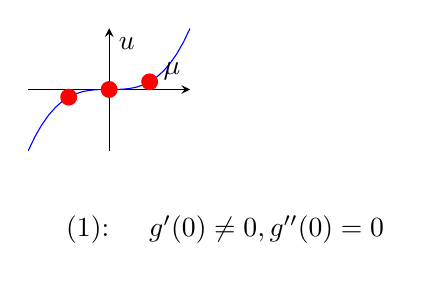
\begin{tikzpicture}
        \begin{axis}
            [
                width=0.3\textwidth,
                axis lines=middle,
                no markers,
                domain=-2:2,
                xtick=\empty,
                ytick=\empty,
                xlabel={$\mu$},
                ylabel={$u$}
            ]
            \addplot[blue] {x^3};
            \coordinate (O) at (axis cs: 0, 0);
            \coordinate (r) at (axis cs: 1, 1);
            \coordinate (l) at (axis cs: -1, -1);
        \end{axis}

        \draw[red, fill] (O) circle (0.1);
        \draw[red, fill] (r) circle (0.1);
        \draw[red, fill] (l) circle (0.1);

        %\draw[blue, thick, domain=0:5, samples=20] plot (\x, {2.5 + 2.5*sin((\x-2.5)*180/5)}) node[right] {$\mu=g(u)$};

        \node at (2.5, -1) {(1): \quad $g'(0)\neq 0, g''(0) = 0$};
    \end{tikzpicture}
    \hspace*{1cm}
    % Left parabola
    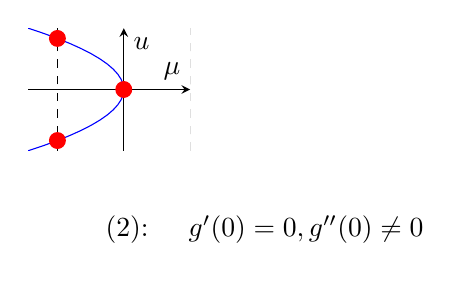
\begin{tikzpicture}
        \begin{axis}[
                width=0.3\textwidth,
                no markers,
                axis lines=middle,
                domain=-1.2:1.2,
                xtick=\empty,
                ytick=\empty,
                xlabel={$\mu$},
                ylabel={$u$}]
            \addplot[blue] ({-x^2}, x);

            \addplot[dashed] ({-1}, x);
            \addplot[dashed] ({1}, x);

            \coordinate (u1) at (axis cs:-1, -1);
            \coordinate (u2) at (axis cs:-1, 1);
            \coordinate (o) at (axis cs:0, 0);
        \end{axis}
        \draw[red, fill] (u1) circle (0.1);
        \draw[red, fill] (u2) circle (0.1);
        \draw[red, fill] (o) circle  (0.1);

        \node at (3, -1) {(2): \quad $g'(0) = 0, g''(0) \neq 0$};
    \end{tikzpicture}
    \hspace{1cm}
    % Line 
    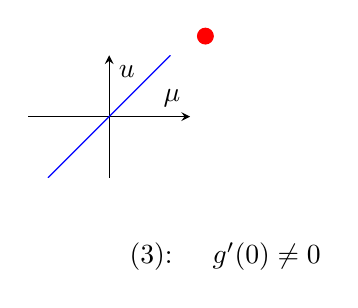
\begin{tikzpicture}
        \begin{axis}[
                width=0.3\textwidth,
                axis equal,
                axis lines=middle,
                no markers,
                xlabel={$\mu$},
                ylabel={$u$},
                xtick=\empty,
                ytick=\empty,
            ]
            \addplot[blue, smooth, domain=-5:5, samples=20] {x};

        \end{axis}

        \draw[red, fill] (2.25, 1.8) circle (0.1);

        \node at (2.5, -1) {(3): \quad $g'(0) \neq0$};
    \end{tikzpicture}

\end{center}

On the left, we gave a unique equilibrium for $\mu$ near $0$. On the right, as $\mu$ increases, two equilibria collide at $\mu =0$ and disappear. Notice that this is different than the case in the logistic model from HW where only one equilibrium disappeared and from the bead on a loop example where two equilibria merged. In some sense, this is a more complicated bifurcation, but also the most common in applications.


\section{Jan 31}
\tbf{Setup:} $u = 0$ is a non-hyperbolic equilibrium at $\mu = 0$, i.e. $f(0, 0) = 0$ and $f_u(0, 0) = 0$.  We want to find solutions of $f = f(u, \mu)$.

Making the assumption, $f_{\mu}(0, 0) = a \neq 0$, we show that $f(u, \mu)=  0$ for $(u, \mu)$ near $(0, 0)$ iff $\mu = g(u)$ with $g(0) = 0$ and $g \in C^{\infty}$.

Formulated differently,we know that $f(u, g(u)) = 0$ for all $u$. Differentiating in $u$, we get
\[0 = \frac{d}{du}(f(u, g(u))) = f_u(u, g(u)) + f_{\mu}(u, g(u))g'(u) \tag{(*)}\]
for all $u$ near $0$

Evaluating at $u = 0$,
\[0 = f_u(0, 0) + f_{\mu}(0, 0)g'(0) = ag'(0) \implies g'(0) = 0\]

From (*), we know that case (1) above is impossible. Can we determine $g''(0)$?

Differentiating again,
\begin{align*}
    0 & = f_u(u, g(u)) + f_{\mu}(u, g(u))g'(u)                                                                                        \\
    0 & = f_{uu}(u, g(u)) + f_{u \mu}(u, g(u))g'(u) + f_{\mu u}(u, g(u)) g'(u) + f_{\mu \mu}(u, g(u))g'(u)^2 + f_{\mu}(u, g(u))g''(u) \\
\end{align*}

Evaluating at $u = 0$,
\begin{align*}
    0 & = f_{uu}(0, 0) + 2f_{u\mu}(0, 0 ) g'(0) + f_{\mu\mu}(0, 0)g''(0)^2 + f_{\mu}(0, 0)g''(0) \\
      & = f_{uu}(0, 0) + f_{\mu}(0, 0)g''(0)
    g''(0) = -\frac{f_{uu}(0, 0)}{f_{\mu}(0, 0)}
\end{align*}

We assume $f_{uu}(0, 0) \neq 0$ to put us in Case (2) above.

\tbf{Remark:} there is no reason we could not have chosen $f_{uu}(0, 0) = 0$ to look at (3). However, in some sense Case (2) is more interesting and also has less tedious calculations. Further, it would be somewhat surprising for there to be neither first nor second derivatives in a Taylor Expansion. In general, though, this choice was arbitrary.

In particular,
\[g(u) = -\frac{1}{2} \frac{f_u(0, 0)}{f_{\mu}(0, 0)} u^2 + O(u^3)\]

\tbf{Conclusion (Existence):} Assume $f(0, 0) = 0, f_u(0, 0) = 0, f_{\mu}(0, 0) \neq 0, f_{uu}(0, 0) \neq 0$. Then $f(u, \mu) = 0$ vanishes near $(0, 0)$ iff $\mu = g(u)$ with $g = -\frac{1}{2} \frac{f_u(0, 0)}{f_{\mu}(0, 0)} u^2 + O(u^3)$.

\subsection{Bifurcation Analysis}

Here, $-\frac{f_u(0, 0)}{f_{\mu}(0, 0)} < 0$ and $\mu < 0$ corresponds to having precisely two rest states, while $\mu > 0$ has none.

The prototypical equation which satisfies our hypothesis is
\[f(u, \mu) = \mu - u^2\]

This gives three possible graphs:

\begin{center}
    \begin{tikzpicture}
        \begin{axis}[
                width=0.3\textwidth,
                axis lines=middle,
                axis equal,
                no markers,
                domain=-1.2:1.2,
                xtick=\empty,
                ytick=\empty]

            \addplot[blue, samples=20] {-x^2} node[below left] {$f(u, 0) = -u^2$};

            \coordinate (O) at (axis cs: 0, 0);
            \coordinate (l) at (axis cs: -0.5, 0);
            \coordinate (r) at (axis cs: 0.5, 0);
        \end{axis}

        \node[orange, scale=2] at (l) {$<$};
        \node[orange, scale=2] at (r) {$<$};

        \draw[red, fill] (O) circle (0.1);

        \node at (3, -1) {$\mu = 0$};
    \end{tikzpicture}
    \hspace{0.5cm}
    \begin{tikzpicture}
        \begin{axis}[
                width=0.3\textwidth,
                axis lines=middle,
                axis equal,
                no markers,
                domain=-1.2:1.2,
                xtick=\empty,
                ytick=\empty]

            \addplot[blue, samples=20] {-x^2 - 1} node[below left] {$f(u, \mu)$};

            \coordinate (O) at (axis cs: 0, 0);
        \end{axis}

        \node at (3, -1) {$\mu < 0$};
    \end{tikzpicture}
    \hspace{0.5cm}
    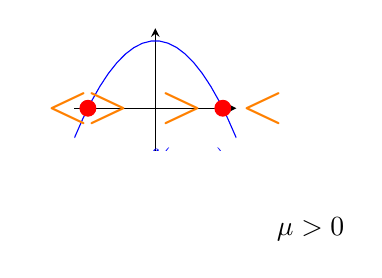
\begin{tikzpicture}
        \begin{axis}[
                width=0.3\textwidth,
                axis lines=middle,
                axis equal,
                no markers,
                domain=-1.2:1.2,
                xtick=\empty,
                ytick=\empty]

            \addplot[blue, samples=20] {-x^2 + 1} node[below left] {$f(u,\mu)$};

            \coordinate (O1) at (axis cs: -1, 0);
            \coordinate (O2) at (axis cs: 1, 0);

            \coordinate (l1) at (axis cs: -1.3, 0);
            \coordinate (r1) at (axis cs: -0.7, 0);
            \coordinate (l2) at (axis cs: 1.6, 0);
            \coordinate (r2) at (axis cs: 0.4, 0);
        \end{axis}

        \node[orange, scale=2] at (l1) {$<$};
        \node[orange, scale=2] at (r1) {$>$};
        \node[orange, scale=2] at (l2) {$<$};
        \node[orange, scale=2] at (r2) {$>$};

        \draw[red, fill] (O1) circle (0.1);
        \draw[red, fill] (O2) circle (0.1);

        \node at (3, -1) {$\mu > 0$};
    \end{tikzpicture}


\end{center}

Which yields the bifurcation diagram:
\begin{center}
    % Left parabola
    \begin{tikzpicture}
        \begin{axis}[no markers,
                axis lines=middle,
                domain=-1.2:1.2,
                xtick=\empty,
                ytick=\empty,
                clip=false]
            \addplot[blue] ({x^2}, x);

            \addplot[dashed] ({-1}, x) node[above] {$\mu < 0$};
            \addplot[dashed] ({1}, x) node[above] {$\mu > 0$};

            \coordinate (u1) at (axis cs:1, -1);
            \coordinate (u2) at (axis cs:1, 1);
            \coordinate (o) at (axis cs:0, 0);
        \end{axis}
        \draw[red, fill] (u1) circle (0.1);
        \draw[red, fill] (u2) circle (0.1);
        \draw[red, fill] (o) circle  (0.1);

        \node[orange, scale=1.5] at (5.6, 0) {\rotatebox{180}{$\wedge$}};
        \node[orange, scale=1.5] at (5.6, 0.9) {$\wedge$};

        \node[orange, scale=1.5] at (5.6, 5.7) {$\wedge$};
        \node[orange, scale=1.5] at (5.6, 4.7) {\rotatebox{180}{$\wedge$}};

        \node[orange, scale=1.5] at (0, 4.7) {\rotatebox{180}{$\wedge$}};
        \node[orange, scale=1.5] at (0, 1.5) {\rotatebox{180}{$\wedge$}};

        \node at (3, -1) {(2): \quad $g'(0) = 0, g''(0) \neq 0$};
    \end{tikzpicture}

\end{center}


\subsection{Stability at the Equilibria}
If $u = u_*$ is an equilibrium of $\dot u = f(u, \mu)$ at $\mu = \mu_*$, then
\[\begin{cases}
        f_u(u_*, \mu_*) > 0 & \text{unstable}     \\
        f_u(u_*, \mu_*) < 0 & \text{stable}       \\
        f_u(u_*, \mu_*) = 0 & \text{undetermined}
    \end{cases}\]

We know that our equilibria occur at $(u, \mu) = (u, g(u))$. Hence, we must check the condition $f_u(u, g(u))$. The process is the same as before:

Take the Taylor Expansion:
\begin{align*}
    f(u, \mu)   & = f_{\mu}(0, 0) \mu + \frac{f_{uu}(0, 0)}{2} u^2 + O(\mu u + \mu^2 + u^3) \\
    f_u(u, \mu) & = f_{uu}(0, 0)u + O(\mu + u^2)                                            \\
\end{align*}

Taking $g(\mu) = -\frac{f_{uu}(0, 0)}{f_{\mu}(0, 0)}u^2 + O(u^3) = O(u^2)$, notice that evaluating $f_u(u, \mu)$ at $(u, \mu) = (u, g(u))$,
\[O(\mu + u^2) = O(g(u) + u^2) = O(u^2)\]
so
\[f_u(u, g(u)) = f_{uu}(0,0)u + O(u^2)\]

Hence, the equilibrium $u$ at $\mu = g(u)$ is
\begin{itemize}
    \item stable for $f_{uu}(0, 0) u < 0$
    \item unstable for $f_{uu}(0, 0) u > 0$
\end{itemize}

\section{Feb 3}
\begin{tbox}{\textbf{Theorem (saddle-node/fold/turning-point bifurcation):} Consider $\dot u = f(u, \mu)$ with $u, \mu\in \R$ and $f \in C^{2}$. Assume that $u_0$ is a non-hyperbolic equilibrium at $\mu = \mu_0$ with $f(u_0, \mu_0) = 0$ and $f_u(u_0, \mu_0) = 0$. Assume further non-degeneracy conditions $f_{uu}(u_0, \mu_0) \neq 0$ and $f_{\mu}(u_0, \mu_0) \neq 0$.

        Then there exist open intervals $I, J$ with $(u_0, \mu_0) \in I \times J$ and a unique $g: I \to J$ with $g(u_0) = \mu_0$ so that $f(u, \mu) = 0$ for $(u, \mu) \in I \times J$ iff $\mu = g(u)$ for some $u \in I$.

        Furthermore, $g \in C^2$ with
        \[g(u) = -\frac{1}{2} \frac{f_{uu}(u_0, \mu_0)}{f_{\mu}(u_0, \mu_0)} (u - u_0)^2 + O(\abs{u - u_0}^3)\]
        and
        \[f_u(u, g(u)) = f_{uu}(u_0, \mu_0) (u - u_0) + O(\abs{u - u_0}^2)\]
        so that $u$ is stable if $f_{uu}(u_0, \mu_0) (u - u_0) < 0$ and unstable if $f_{uu}(u_0, \mu_0) (u - u_0) > 0$.}
    \emph{Proof:} Follows from example above
\end{tbox}

\tbf{Example:} Assume
\[\begin{cases}
        f_{\mu} (u_0, \mu_0) > 0 \\
        f_{uu}(u_0, \mu_0) < 0
    \end{cases}\]

Then
\[g(u) = \underbrace{-\frac{1}{2} \frac{f_{uu}(u_0, \mu_0)}{f_{\mu}(u_0, \mu_0)}}_{< 0} (u - u_0)^2 + O(\abs{u - u_0}^3)\]
hence $u$ is stable if $u < u_0$ and unstable if $u > u_0$.

\begin{center}
    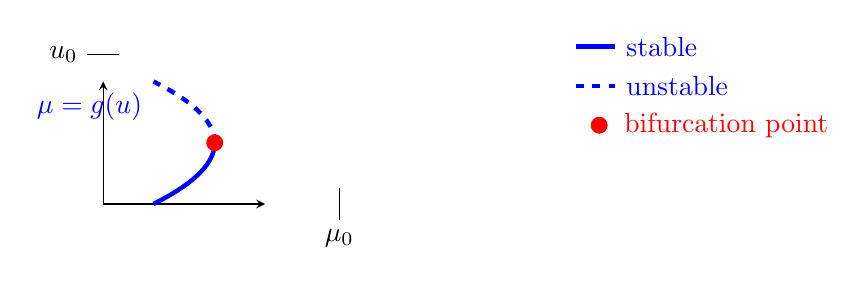
\begin{tikzpicture}
        \begin{axis}[
                width=0.3\textwidth,
                axis lines=left,
                axis equal,
                no markers,
                domain=-1.2:1.2,
                xtick=\empty,
                ytick=\empty,
                clip=false]

            \addplot[blue, ultra thick, dashed, domain=0:1,  samples=20] ({-x^2}, {x}) node[below left] {$\mu = g(u)$};
            \addplot[blue, ultra thick, domain=-1:0,  samples=20] ({-x^2}, {x}) ;


            \coordinate (O) at (axis cs: 0, 0);

        \end{axis}

        \draw (3, 0.2) -- (3, -0.2) node[below] {$\mu_0$};
        \draw (0.2, 1.9) -- (-0.2, 1.9) node[left] {$u_0$};

        \draw[red, fill] (O) circle (0.1);

        \draw[blue, ultra thick] (6, 2) -- (6.5, 2) node[right] {stable};
        \draw[blue, ultra thick, dashed] (6, 1.5) -- (6.5, 1.5) node[right] {unstable};
        \draw[red, fill] (6.3, 1) circle (0.1) node[right]{\;\;bifurcation point};

    \end{tikzpicture}
\end{center}

An important question is how we know that the $O(u^3)$ terms do not change the graph of $u$ dramatically.

Consider
\[g(u) = u^2 + O(u^3) = (1 + O(u))u^2\]
so
\[\begin{cases}
        g(0) = 0  \\
        g'(0) = 0 \\
        g''(0) = 2
    \end{cases}\]

Hence:
\begin{center}
    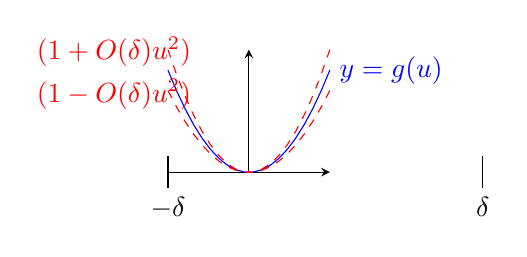
\begin{tikzpicture}
        \begin{axis}[
                width=0.3\textwidth,
                axis lines=middle,
                no markers,
                domain=-1.2:1.2,
                xtick=\empty,
                ytick=\empty,
                clip=false]

            \addplot[blue, samples=20] {x^2} node[right] {$y = g(u)$};
            \addplot[red, dashed, samples=20] {0.8*x^2};
            \addplot[red, dashed, samples=20] {1.2*x^2};

            \node[red] at (axis cs: -2, 1.7) {$(1 + O(\delta)u^2$)};
            \node[red] at (axis cs: -2, 1.1) {$(1 - O(\delta)u^2$)};

        \end{axis}

        \draw (4, 0.2) -- (4, -0.2) node[below] {$\delta$};
        \draw (0, 0.2) -- (0, -0.2) node[below] {$-\delta$};

    \end{tikzpicture}
\end{center}

\subsection{Summary of Bifurcations (so far):}
\begin{itemize}
    \item Pitchfork bifurcation

          \begin{center}
              % Right Parabola
              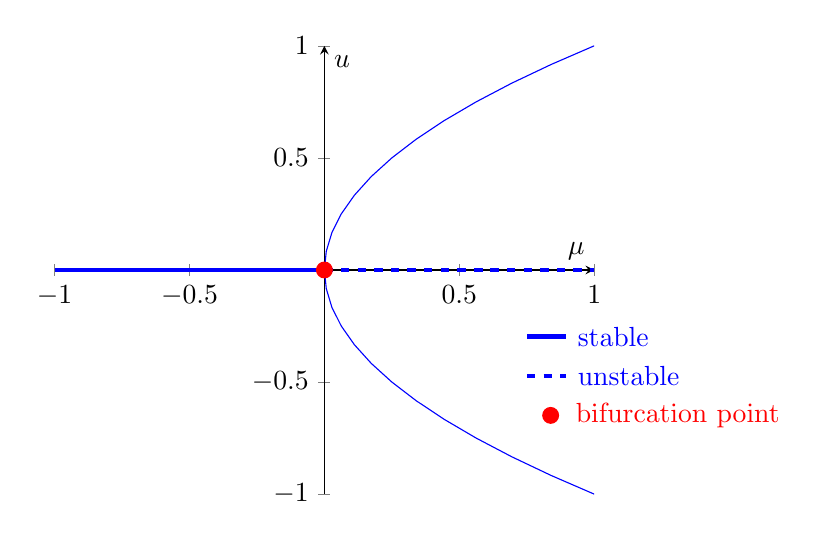
\begin{tikzpicture}
                  \begin{axis}[
                          no markers,
                          axis lines=middle,
                          domain=-2:2,
                          xlabel={$\mu$},
                          ylabel={$u$}]
                      \addplot[blue, domain=-1:1] ({x^2}, x);

                      \addplot[blue, ultra thick, domain=-1:0] {0};
                      \addplot[blue, ultra thick, dashed, domain=0:1] {0};

                      \coordinate (pt) at (axis cs: 0, 0);
                  \end{axis}

                  \draw[red, fill] (pt) circle (0.1);

                  \draw[blue, ultra thick] (6, 2) -- (6.5, 2) node[right] {stable};
                  \draw[blue, ultra thick, dashed] (6, 1.5) -- (6.5, 1.5) node[right] {unstable};
                  \draw[red, fill] (6.3, 1) circle (0.1) node[right]{\;\;bifurcation point};
              \end{tikzpicture}
          \end{center}

    \item Transitional Bifurcation

          \begin{center}
              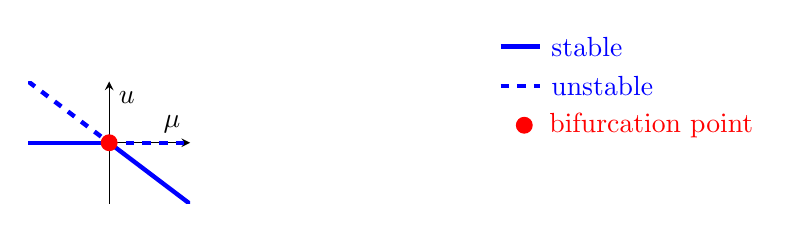
\begin{tikzpicture}
                  \begin{axis}
                      [
                          width=0.3\textwidth,
                          axis lines=middle,
                          no markers,
                          domain=-2:2,
                          xtick=\empty,
                          ytick=\empty,
                          xlabel={$\mu$},
                          ylabel={$u$}
                      ]
                      \addplot[blue, ultra thick, dashed, domain=-2:0] {-x};
                      \addplot[blue, ultra thick, domain=0:2] {-x};

                      \addplot[blue, ultra thick, domain=-2:0] {0};
                      \addplot[blue, ultra thick, dashed, domain=0:2] {0};


                      \coordinate (O) at (axis cs: 0, 0);

                  \end{axis}
                  \draw[fill, red] (O) circle (0.1);

                  \draw[blue, ultra thick] (6, 2) -- (6.5, 2) node[right] {stable};
                  \draw[blue, ultra thick, dashed] (6, 1.5) -- (6.5, 1.5) node[right] {unstable};
                  \draw[red, fill] (6.3, 1) circle (0.1) node[right]{\;\;bifurcation point};
              \end{tikzpicture}
          \end{center}

    \item Fold/turning-point/saddle-node Bifurcation

          \begin{center}
              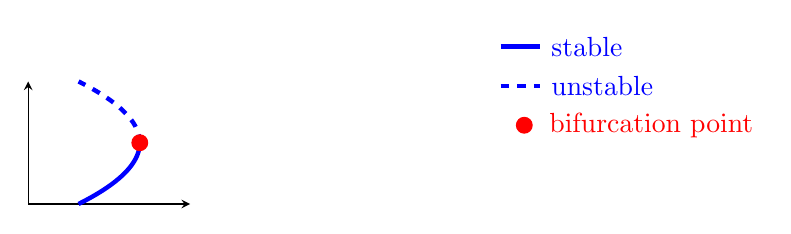
\begin{tikzpicture}
                  \begin{axis}[
                          width=0.3\textwidth,
                          axis lines=left,
                          axis equal,
                          no markers,
                          domain=-1.2:1.2,
                          xtick=\empty,
                          ytick=\empty,
                          clip=false]

                      \addplot[blue, ultra thick, dashed, domain=0:1,  samples=20] ({-x^2}, {x});
                      \addplot[blue, ultra thick, domain=-1:0,  samples=20] ({-x^2}, {x}) ;


                      \coordinate (O) at (axis cs: 0, 0);

                  \end{axis}

                  \draw[red, fill] (O) circle (0.1);

                  \draw[blue, ultra thick] (6, 2) -- (6.5, 2) node[right] {stable};
                  \draw[blue, ultra thick, dashed] (6, 1.5) -- (6.5, 1.5) node[right] {unstable};
                  \draw[red, fill] (6.3, 1) circle (0.1) node[right]{\;\;bifurcation point};

              \end{tikzpicture}
          \end{center}
\end{itemize}

\section{Feb 5}
\subsection{When do we expect to encounter these bifurcations?}
\begin{itemize}
    \item \tbf{Saddle-node Bifurcation:}
          \[\begin{cases}
                  f(u_0, \mu_0) = 0         \\
                  f_u(u_0, \mu_0) = 0       \\
                  f_{uu}(u_0, \mu_0) \neq 0 \\
                  f_{\mu}(u_0, \mu_0) \neq 0
              \end{cases}\]
          which has prototypical example $\dot u = \mu - u^2 = f(u, \mu)$:

          \begin{center}
              % Left parabola
              \begin{tikzpicture}
                  \begin{axis}[no markers,
                          axis lines=middle,
                          domain=-1.2:1.2,
                          xtick=\empty,
                          ytick=\empty,
                          clip=false,
                          xlabel={$\mu$},
                          ylabel={$u$}]
                      \addplot[blue, domain=0:1.2] ({x^2}, x);
                      \addplot[blue, dashed, domain=-1.2:0] ({x^2}, x);


                      \addplot[dashed] ({-1}, x);
                      \addplot[dashed] ({1}, x);

                      \coordinate (u1) at (axis cs:1, -1);
                      \coordinate (u2) at (axis cs:1, 1);
                      \coordinate (o) at (axis cs:0, 0);
                  \end{axis}
                  \draw[red, fill] (u1) circle (0.1);
                  \draw[red, fill] (u2) circle (0.1);
                  \draw[red, fill] (o) circle  (0.1);

                  \node[orange, scale=1.5] at (5.6, 0) {\rotatebox{180}{$\wedge$}};
                  \node[orange, scale=1.5] at (5.6, 0.9) {$\wedge$};

                  \node[orange, scale=1.5] at (5.6, 5.7) {$\wedge$};
                  \node[orange, scale=1.5] at (5.6, 4.7) {\rotatebox{180}{$\wedge$}};

                  \node[orange, scale=1.5] at (0, 4.7) {\rotatebox{180}{$\wedge$}};
                  \node[orange, scale=1.5] at (0, 1.5) {\rotatebox{180}{$\wedge$}};

                  \node[orange, scale=1.5] at (2.8, 4.7) {\rotatebox{180}{$\wedge$}};
                  \node[orange, scale=1.5] at (2.8, 1.5) {\rotatebox{180}{$\wedge$}};

              \end{tikzpicture}
          \end{center}

          and phase diagrams:

          \begin{center}
              \begin{tikzpicture}
                  \begin{axis}[
                          width=0.3\textwidth,
                          axis lines=middle,
                          axis equal,
                          no markers,
                          xtick=\empty,
                          ytick=\empty,
                          ymin=-2, ymax=2]


                      \addplot[blue, samples=40] {-x^2} ;

                      \coordinate (O) at (axis cs: 0, 0);
                      \coordinate (l) at (axis cs: -0.5, 0);
                      \coordinate (r) at (axis cs: 0.5, 0);
                  \end{axis}

                  \node[orange] at (l) {$<$};
                  \node[orange] at (r) {$<$};

                  \draw[red, fill] (O) circle (0.1);

                  \node at (2.5, -1) {$\mu = 0$};
              \end{tikzpicture}
              \hspace{0.5cm}
              \begin{tikzpicture}
                  \begin{axis}[
                          width=0.3\textwidth,
                          axis lines=middle,
                          axis equal,
                          no markers,
                          xtick=\empty,
                          ytick=\empty,
                          ymin=-2, ymax=2]

                      \addplot[blue, samples=20] {-x^2 - 1};

                      \coordinate (O) at (axis cs: 0, 0);
                  \end{axis}

                  \node at (2.5, -1) {$\mu < 0$};
              \end{tikzpicture}
              \hspace{0.5cm}
              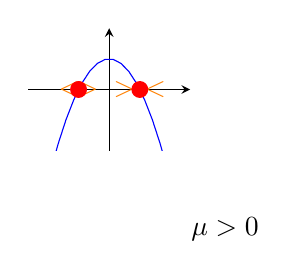
\begin{tikzpicture}
                  \begin{axis}[
                          width=0.3\textwidth,
                          axis lines=middle,
                          axis equal,
                          no markers,
                          xtick=\empty,
                          ytick=\empty,
                          ymin=-2, ymax=2]

                      \addplot[blue, samples=40] {-x^2 + 1};

                      \coordinate (O1) at (axis cs: -1, 0);
                      \coordinate (O2) at (axis cs: 1, 0);

                      \coordinate (l1) at (axis cs: -1.3, 0);
                      \coordinate (r1) at (axis cs: -0.7, 0);
                      \coordinate (l2) at (axis cs: 1.5, 0);
                      \coordinate (r2) at (axis cs: 0.5, 0);
                  \end{axis}

                  \node[orange] at (l1) {$<$};
                  \node[orange] at (r1) {$>$};
                  \node[orange] at (l2) {$<$};
                  \node[orange] at (r2) {$>$};

                  \draw[red, fill] (O1) circle (0.1);
                  \draw[red, fill] (O2) circle (0.1);

                  \node at (2.5, -1) {$\mu > 0$};
              \end{tikzpicture}


          \end{center}



          In some sense, these are the bifurcations we expect to see most often.

    \item \tbf{Transcritical bifurcation:}
          \[\begin{cases}
                  f(0, 0) = 0   & \text{existence of equilibrium} \\
                  f(0, \mu) = 0 \quad \forall \mu                 \\
                  f_u(0, 0) = 0 & \text{non-hyperbolic}           \\
                  f_{u\mu}(0, 0) \neq 0                           \\
                  f_{uu}(0, 0) \neq 0                             \\
              \end{cases}\]

          The essential character here is that there always an equilibrium at $u = 0$. Hence, the prototypical example is $\dot u = u(u - \mu) = f(u, \mu)$

          \begin{center}
              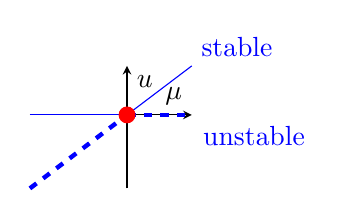
\begin{tikzpicture}
                  \begin{axis}[
                          width=0.3\textwidth,
                          axis lines=middle,
                          no markers,
                          domain=-3:2,
                          xtick=\empty,
                          ytick=\empty,
                          xlabel={$\mu$},
                          ylabel={$u$},
                          clip=false
                      ]
                      \addplot[blue, domain=0:2] {x} node[above right] {stable};
                      \addplot[blue, dashed, ultra thick, domain=-3:0] {x};

                      \addplot[blue, domain=-3:0] {0};
                      \addplot[blue, ultra thick, dashed, domain=0:2] {0} node[below right] {unstable};


                      \coordinate (O) at (axis cs: 0, 0);
                  \end{axis}
                  \draw[red, fill] (O) circle (0.1);
              \end{tikzpicture}
          \end{center}

          Which has phase diagrams:
          \begin{center}
              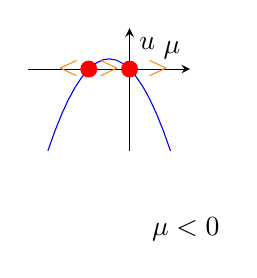
\begin{tikzpicture}
                  \begin{axis}[
                          width=0.3\textwidth,
                          axis lines=middle,
                          no markers,
                          domain=-2.5:1.5,
                          xtick=\empty,
                          ytick=\empty,
                          xlabel={$\mu$},
                          ylabel={$u$},
                          axis equal,
                          ymin=-2, ymax=1
                      ]
                      \addplot {-x*(x+1)};

                      \coordinate (O) at (axis cs: 0, 0);
                      \coordinate (l) at (axis cs: -1, 0);

                      \coordinate (l1) at (axis cs: -1.5, 0);
                      \coordinate (r1) at (axis cs: -0.5, 0);

                      \coordinate (r2) at (axis cs: 0.7, 0);
                  \end{axis}
                  \draw[red, fill] (O) circle (0.1);
                  \draw[red, fill] (l) circle (0.1);

                  \node[orange] at (l1) {$<$};
                  \node[orange] at (r1) {$>$};
                  \node[orange] at (r2) {$>$};

                  \node at (2, -1) {$\mu < 0$};
              \end{tikzpicture}
              \hspace{0.5cm}
              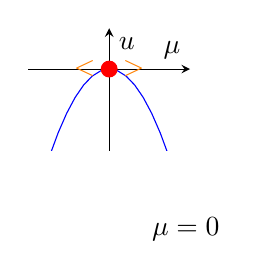
\begin{tikzpicture}
                  \begin{axis}[
                          width=0.3\textwidth,
                          axis lines=middle,
                          no markers,
                          domain=-2.5:2.5,
                          xtick=\empty,
                          ytick=\empty,
                          xlabel={$\mu$},
                          ylabel={$u$},
                          axis equal,
                          ymin=-2, ymax=1
                      ],
                      \addplot {-x^2};
                      \coordinate (O) at (axis cs: 0, 0);

                      \coordinate (l) at (axis cs: -0.6, 0);
                      \coordinate (r) at (axis cs: 0.6, 0);
                  \end{axis}
                  \draw[red, fill] (O) circle (0.1);

                  \node[orange] at (l) {$<$};
                  \node[orange] at (r) {$>$};

                  \node at (2, -1) {$\mu = 0$};

              \end{tikzpicture}
              \hspace{0.5cm}
              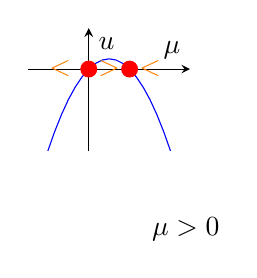
\begin{tikzpicture}
                  \begin{axis}[
                          width=0.3\textwidth,
                          axis lines=middle,
                          no markers,
                          domain=-1.5:2.5,
                          xtick=\empty,
                          ytick=\empty,
                          xlabel={$\mu$},
                          ylabel={$u$},
                          axis equal,
                          ymin=-2, ymax=1
                      ]
                      \addplot {-x*(x-1)};

                      \coordinate (O) at (axis cs: 0, 0);
                      \coordinate (O1) at (axis cs: 1, 0);

                      \coordinate (l) at (axis cs: -0.7, 0);
                      \coordinate (r1) at (axis cs: 0.5, 0);
                      \coordinate (r2) at (axis cs: 1.5, 0);

                  \end{axis}
                  \draw[red, fill] (O) circle (0.1);
                  \draw[red, fill] (O1) circle (0.1);

                  \node[orange] at (l) {$<$};
                  \node[orange] at (r1) {$>$};
                  \node[orange] at (r2) {$<$};


                  \node at (2, -1) {$\mu > 0$};

              \end{tikzpicture}
          \end{center}

    \item \tbf{Pitchfork Bifurcation:}
          \[\begin{cases}
                  f(-u, \mu) = -f(u, \mu) \quad \forall (u, \mu) & \text{ odd in } u     \\
                  f_u(0, 0) = 0                                  & \text{non-hyperbolic} \\
                  f_{u\mu}(0, 0) \neq 0                          & \text{non-degenerate} \\
                  f_{uuu}(0, 0) \neq 0                           & \text{non-degenerate}
              \end{cases}\]
          where the first condition comes from the fact that the Taylor Series contains only odd powers of $u$.

          This has two possible bifurcation diagrams:
          \begin{center}
              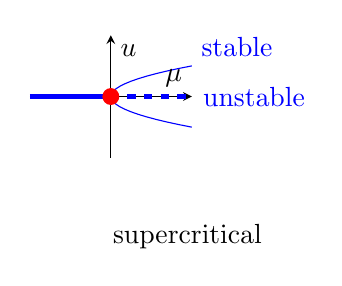
\begin{tikzpicture}
                  \begin{axis}[
                          width=0.3\textwidth,
                          axis lines=middle,
                          no markers,
                          domain=-1:1,
                          xtick=\empty,
                          ytick=\empty,
                          clip=false,
                          xlabel={$\mu$},
                          ylabel={$u$},
                          ymin=-2, ymax=2
                      ]

                      \addplot[blue, ultra thick, domain=-1:0] {0};
                      \addplot[blue, ultra thick, dashed, domain=0:1] {0} node[right] {unstable};

                      \addplot[blue] ({x^2}, {x}) node[above right] {stable};

                      \coordinate (O) at (axis cs: 0, 0);
                  \end{axis}
                  \draw[fill, red] (O) circle (0.1);

                  \node at (2, -1) {supercritical};
              \end{tikzpicture}
              \hspace{1cm}
              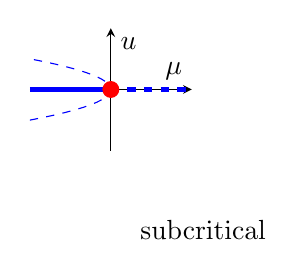
\begin{tikzpicture}
                  \begin{axis}[
                          width=0.3\textwidth,
                          axis lines=middle,
                          no markers,
                          domain=-1:1,
                          xtick=\empty,
                          ytick=\empty,
                          clip=false,
                          xlabel={$\mu$},
                          ylabel={$u$},
                          ymin=-2, ymax=2
                      ]
                      \addplot[blue, ultra thick, domain=-1:0] {0};
                      \addplot[blue, ultra thick, dashed, domain=0:1] {0};

                      \addplot[blue, dashed] ({-x^2}, {x});

                      \coordinate (O) at (axis cs: 0, 0);
                  \end{axis}
                  \draw[fill, red] (O) circle (0.1);

                  \node at (2.2, -1) {subcritical};
              \end{tikzpicture}
          \end{center}

          The prototypical example is $\dot u = u(\mu = u^2) = f(u, \mu)$ which has phase diagrams:
          \begin{center}
              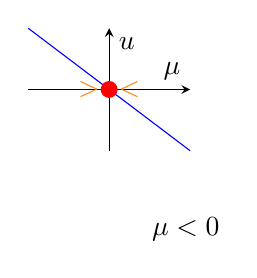
\begin{tikzpicture}
                  \begin{axis}[
                          width=0.3\textwidth,
                          axis lines=middle,
                          no markers,
                          domain=-2:2,
                          xtick=\empty,
                          ytick=\empty,
                          clip=false,
                          xlabel={$\mu$},
                          ylabel={$u$},
                          ymin=-2, ymax=2
                      ]
                      \addplot[blue] {-x};

                      \coordinate (O) at (axis cs: 0, 0);
                      \coordinate (l) at (axis cs: -0.5, 0);
                      \coordinate (r) at (axis cs: 0.5, 0);

                  \end{axis}
                  \draw[red, fill] (O) circle (0.1);

                  \node[orange] at (l) {$>$};
                  \node[orange] at (r) {$<$};

                  \node at (2, -1) {$\mu < 0$};
              \end{tikzpicture}
              \hspace{0.5cm}
              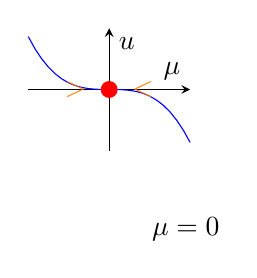
\begin{tikzpicture}
                  \begin{axis}[
                          width=0.3\textwidth,
                          axis lines=middle,
                          no markers,
                          domain=-1.2:1.2,
                          xtick=\empty,
                          ytick=\empty,
                          clip=false,
                          xlabel={$\mu$},
                          ylabel={$u$},
                          ymin=-2, ymax=2
                      ]
                      \addplot[blue] {-x^3};

                      \coordinate (O) at (axis cs: 0, 0);
                      \coordinate (l) at (axis cs: -0.5, 0);
                      \coordinate (r) at (axis cs: 0.5, 0);

                  \end{axis}
                  \draw[red, fill] (O) circle (0.1);

                  \node[orange] at (l) {$>$};
                  \node[orange] at (r) {$<$};

                  \node at (2, -1) {$\mu = 0$};
              \end{tikzpicture}
              \hspace{0.5cm}
              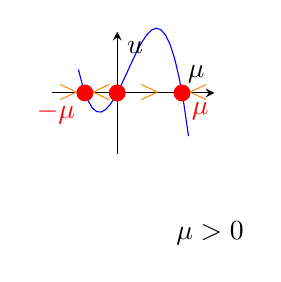
\begin{tikzpicture}
                  \begin{axis}[
                          width=0.3\textwidth,
                          axis lines=middle,
                          no markers,
                          domain=-1.2:2.2,
                          xtick=\empty,
                          ytick=\empty,
                          clip=false,
                          xlabel={$\mu$},
                          ylabel={$u$},
                          ymin=-2, ymax=2,
                          xmin=-2, xmax=3
                      ]
                      \addplot[blue] {-x*(x+1)*(x-2)};

                      \coordinate (O1) at (axis cs: 0, 0);
                      \coordinate (O2) at (axis cs: -1, 0);
                      \coordinate (O3) at (axis cs: 2, 0);

                      \coordinate (l1) at (axis cs: -1.5, 0);
                      \coordinate (r1) at (axis cs: 1, 0);
                      \coordinate (l2) at (axis cs: -0.5, 0);
                      \coordinate (r2) at (axis cs: 2.5, 0);


                  \end{axis}
                  \draw[red, fill] (O1) circle (0.1);
                  \draw[red, fill] (O2) circle (0.1) node[below left] {$-\mu$};
                  \draw[red, fill] (O3) circle (0.1) node[below right] {$\mu$};

                  \node[orange] at (l1) {$>$};
                  \node[orange] at (r1) {$>$};
                  \node[orange] at (l2) {$<$};
                  \node[orange] at (r2) {$<$};


                  \node at (2, -1) {$\mu > 0$};
              \end{tikzpicture}
          \end{center}
\end{itemize}

\tbf{Remark:} Transcritical and pitchfork bifurcations only occur for equilibria at $0$

What happens if one of the non-degeneracy conditions ($f_{\mu}(0, 0) = 0, \; f_{uu}(0, 0) = 0$) is not true? In general, this suggests that the system has another parameter and we might need to consider variations in multiple parameters around the points. In general, this gets very complicated, very fast and we do not yet have a full model.

\section{Feb 5}
\subsection{Population model for Budworms}
\tbf{PART 1: Nondimensionalize}

Let $N$ be the population density. Hence, as normal,
\[\frac{dN}{dt} = RN(1 - \frac{N}{k}) - \frac{BN^2}{A + N^2}\]
where $B$ is the capacity for predator eating and on (*), the predators search for an alternative food source.

\begin{center}
    \begin{tikzpicture}
        \begin{axis}[
                width=0.3\textwidth,
                axis lines=middle,
                no markers,
                domain=0:4,
                xtick=\empty,
                ytick=\empty,
                clip=false,
                xlabel={$N$},
                ylabel={$\frac{dN}{dt}$},
                ymin=0, ymax=2,
                xmin=0, xmax=5
            ]

            \addplot[blue] {1.5/(1+exp(-5*(x-2)))};
            \addplot[dashed, domain=0:5] {1.5};
            \addplot[red, dashed, ultra thick, domain=0:1] {0} node[midway, below] {*};

        \end{axis}
        \node at (5, 3) {$B$};

    \end{tikzpicture}
\end{center}

A reasonable first step is to non-dimensionalize the system. We currently have units of
\begin{itemize}
    \item $R$: $\frac{1}{\text{time}}$
    \item $K$: population
    \item $A$: population
    \item $B$: $\frac{\text{population}}{\text{time}}$
\end{itemize}

Hence, let $x = \frac{N}{A}$, so
\[A \dot x = ARx(1 - \frac{Ax}{K}) - \frac{Bx^2}{1 + x^2}\]

To non-dimensionalize time, we would also like to reduce the parameters. Let $\tau = \frac{B}{A} t$, so
\[\frac{d}{dt} = \frac{d}{d\tau} \frac{d\tau}{dt} = \frac{B}{A} \frac{d}{d\tau}\]
which gives
\[\frac{dx}{d\tau} = \frac{AR}{B} x(1 - \frac{A}{K}x) - \frac{x^2}{1 + x^2} \]

Let $a = \frac{AR}{B} > 0$ represent the growth rate and $b = \frac{K}{A} > 0$ represent the carrying capacity. Hence, our final system is
\[\frac{dx}{d\tau} = ax(1 - \frac{x}{b}) - \frac{x^2}{1 + x^2}\]
and this looks very familiar.

\tbf{PART 2: Bifurcation Analysis}

Let $f(x, a, b) = ax(1 - \frac{x}{b}) - \frac{x^2}{1 + x^2}$
Clearly, $x = 0$ is always an equilibrium. Also, $f_x(0, a, b) = a > 0$ so $x = 0$ is always unstable.

Now it suffices to consider $f(x, a, b) = a(1- \frac{x}{b}) - \frac{x}{1 + x^2}$

\emph{Case 1.} $b \ll$, vary $a$.

\begin{center}
    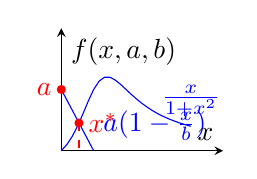
\begin{tikzpicture}
        \begin{axis}[
                width=0.3\textwidth,
                axis lines=middle,
                no markers,
                domain=0:4,
                xtick=\empty,
                ytick=\empty,
                clip=false,
                xlabel={$x$},
                ylabel={$f(x, a, b)$},
                ymin=0, ymax=2,
                xmin=0, xmax=5
            ]

            \addplot[blue] {x/(1+(x-1)^2)} node[above] {$\frac{x}{1+x^2}$};
            \addplot[blue, domain=0:1] {-x+1} node [above right] {$a(1 - \frac{x}{b})$};

            \coordinate (a) at (axis cs: 0, 1);
            \coordinate (pt) at (axis cs: 0.545, 0.453);
            \coordinate (o) at (axis cs: 0.545, 0);

        \end{axis}
        \draw[red, fill] (a) circle (0.05) node[left] {$a$};
        \draw[red, fill] (pt) circle (0.05) node[right] {$x^*$};
        \draw [red, dashed] (pt) -- (o);

    \end{tikzpicture}
\end{center}

\emph{Case 2.} $b \gg$, vary $a$.

\begin{center}
    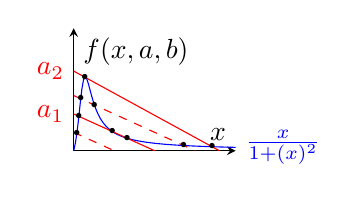
\begin{tikzpicture}
        \begin{axis}[
                width=0.3\textwidth,
                axis lines=middle,
                no markers,
                domain=0:20,
                xtick=\empty,
                ytick=\empty,
                clip=false,
                xlabel={$x$},
                ylabel={$f(x, a, b)$},
                ymin=0, ymax=2,
                xmin=0, xmax=20
            ]

            \addplot[blue, samples=100, name path=blue] {x/(1+(x-1)^2)} node[right] {$\frac{x}{1+(x)^2}$};

            \coordinate (a1) at (axis cs: 0, 0.6);
            \coordinate (a2) at (axis cs: 0, 1.3);

            \addplot[red, name path=red2] plot coordinates {(0, 1.3) (18, 0)};
            \addplot[red, name path=red1] plot coordinates {(0, 0.6) (10, 0)};
            \addplot[red, dashed, name path=red05] plot coordinates {(0, 0.3) (5, 0)};
            \addplot[red, dashed, name path=red15] plot coordinates {(0, 0.9) (15, 0)};

            \fill [name intersections={of=blue and red1, total=\t}]
            \foreach \s in {1,...,\t}{(intersection-\s) node[scale=0.5] {$\bullet$}};

            \fill [name intersections={of=blue and red2, total=\t}]
            \foreach \s in {1,...,\t}{(intersection-\s) node[scale=0.5] {$\bullet$}};

            \fill [name intersections={of=blue and red05, total=\t}]
            \foreach \s in {1,...,\t}{(intersection-\s) node[scale=0.5] {$\bullet$}};

            \fill [name intersections={of=blue and red15, total=\t}]
            \foreach \s in {1,...,\t}{(intersection-\s) node[scale=0.5] {$\bullet$}};

        \end{axis}
        \node[left, red] at (a1) {$a_1$};
        \node[left, red] at (a2) {$a_2$};

    \end{tikzpicture}

    \hspace*{1cm}
    \begin{tabular}{c|c}
        $a$             & number of fixed points \\ \hline
        $a < a_1$       & 1                      \\
        $a = a_1$       & 2 (saddle)             \\
        $a_1 < a < a_2$ & 3                      \\
        $a = a_2$       & 2 (saddle)             \\
        $a > a_2$       & 1                      \\
    \end{tabular}
\end{center}

So at last we can draw our bifurcation diagram:

\begin{center}
    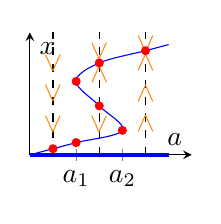
\begin{tikzpicture}
        \begin{axis}[
                width=0.3\textwidth,
                axis lines=middle,
                no markers,
                domain=0:6,
                xtick={2, 4},
                ytick=\empty,
                xticklabels={$a_1$, $a_2$},
                clip=false,
                xlabel={$a$},
                ylabel={$x$},
                ymin=0, ymax=2,
                xmin=0, xmax=7
            ]

            \addplot[blue, ultra thick] {0};

            \addplot[dashed, domain=0:2] ({1}, {x});
            \addplot[dashed, domain=0:2] ({3}, {x});
            \addplot[dashed, domain=0:2] ({5}, {x});

            \coordinate (o) at (axis cs: 0, 0);
            \coordinate (a) at (axis cs: 1, 0.1);
            \coordinate (b) at (axis cs: 2, 0.2);
            \coordinate (c) at (axis cs: 4, 0.4);
            \coordinate (d) at (axis cs: 3, 0.8);
            \coordinate (e) at (axis cs: 2, 1.2);
            \coordinate (f) at (axis cs: 3, 1.5);
            \coordinate (g) at (axis cs: 5, 1.7);


            \node[orange] at (axis cs: 1, 1.5) {\rotatebox{180}{$\wedge$}};
            \node[orange] at (axis cs: 1, 1) {\rotatebox{180}{$\wedge$}};
            \node[orange] at (axis cs: 1, 0.5) {\rotatebox{180}{$\wedge$}};

            \node[orange] at (axis cs: 5, 0.5) {$\wedge$};
            \node[orange] at (axis cs: 5, 1) {$\wedge$};
            \node[orange] at (axis cs: 5, 1.5) {$\wedge$};
            \node[orange] at (axis cs: 5, 1.8) {\rotatebox{180}{$\wedge$}};


            \node[orange] at (axis cs: 3, 0.5) {\rotatebox{180}{$\wedge$}};
            \node[orange] at (axis cs: 3, 1.3) {$\wedge$};
            \node[orange] at (axis cs: 3, 1.7) {\rotatebox{180}{$\wedge$}};
            \draw[blue] plot [smooth, tension=0.6] coordinates {(o) (a) (b) (c) (d) (e) (f) (g) (axis cs: 6, 1.8)};

        \end{axis}

        \draw[red, fill] (a) circle (0.05);
        \draw[red, fill] (b) circle (0.05);
        \draw[red, fill] (c) circle (0.05);
        \draw[red, fill] (d) circle (0.05);
        \draw[red, fill] (e) circle (0.05);
        \draw[red, fill] (f) circle (0.05);
        \draw[red, fill] (g) circle (0.05);

    \end{tikzpicture}

    In this diagram, we call the region $[a_1, a_2]$ \tbf{bistable} because there are two stable equilibria. Population levels on $[0, a_2)$ represent a ``normal'' population level, while the node at $a_2$ represents an insect outbreak when $a > a_2$. At the end of the curve, we say the population is in an ``outbreak'' population level
\end{center}

\tbf{Hysteresis:} If we start with the budworm population on the lower stable branch and slowly increase the parameter $a$, the population will remain on the lower branch until $a = a_2$. Beyond this point, the population will jump to the upper branch (at a much higher population level). Then reducing $a < a_2$ will not restore the lower population level since the population will now follow the upper stable branch until it reaches the bifurcation point at $a_1$.

\chapter{Phase Space}
\section{Feb 10}
Consider systems of ODEs of the form $\dot u = F(u)$ with $u \in \R^n$, $F: \R^n \to \R^n$ and $F \in C^1$/

\tbf{Example:} $u = (u_1, u_2) \in \R^2$.
\[\begin{cases}
        \dot u_1 = u_1(2 - u_1 - 2u_2) = F_1(u_1, u_2) \\
        \dot u_2 = u_2(2 - u_1 - u_2) = F_2(u_1, u_2)
    \end{cases}\]
with $F(u) = F(u_1, u_2) = \begin{pmatrix}
        F_1(u_1, u_2) \\
        F_2(u_1, u_2)
    \end{pmatrix}$.

$F \in C^1$ since $F_1, F_2$ are continuously differentiable in $(u_1, u_2)$.

We can calculate the Jacobian
\[F_u(i) = \begin{pmatrix}
        \frac{\partial F_1}{\partial u_1}(u_1, u_2) & \frac{\partial F_1}{\partial u_2}(u_1, u_2) \\
        \frac{\partial F_2}{\partial u_1}(u_1, u_2) & \frac{\partial F_2}{\partial u_2}(u_1, u_2)
    \end{pmatrix} = \begin{pmatrix}
        3 - 2u_1 - 2u_2 & -2u_1          \\
        -u_2            & 2 - u_1 - 2u_2
    \end{pmatrix}\]

\tbf{Solution:} A function $u: \R \to \R^n$ in $C^1$ is a \emph{solution} of $\dot u = F(u)$ if $\frac{du(t)}{dt} = F(u(t))$ for all $t \in \R$. (Equivalently, we could replace $t \in \R$ by $t \in J$ for some open interval $J \sub \R$)


\subsection{Existence and Uniqueness of Solutions}
For
\[\begin{cases}
        \dot u = F(u) \\
        u(0) = u_0
    \end{cases}\]
let $u \in \R^n$, $F: \R^n \to \R^n$ in $C^1$ with initial condition $u_0 \in \R^n$ given.

\begin{proposition}
    \textbf{Theorem (Existence and Uniqueness):} Assume $F: \R^n \to \R^n$ is $C^1$. For each $u_0 \in \R^n$, there exists a $\delta > 0$ and a unique $u: (-\delta, \delta) \to \R^n$ so that $u \in C^1$ which satisfies the system above for all $t \in (-\delta, \delta)$.

    Furthermore, $\delta$ can be chosen to depend continuously on $u_0$ so the map $u_0 \mapsto u(t;\, u_0)$ is $C^1$ in $u_0$ (where $u(t; \, u_0)$ denotes the unique solution of the system for $t \in (-\delta, \delta)$.)
\end{proposition}

\tbf{Consequences:} Trajectories $\{u(t): t \in \R\}$ cannot touch or cross.

\begin{center}
    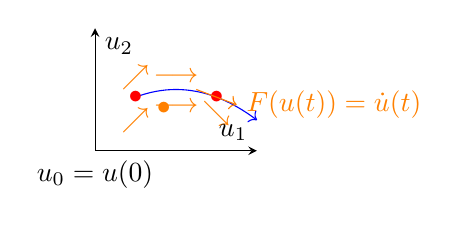
\begin{tikzpicture}
        \begin{axis}[
                width=0.3\textwidth,
                axis lines=middle,
                no markers,
                domain=0:4,
                xtick=\empty,
                ytick=\empty,
                clip=false,
                xlabel={$u_1$},
                ylabel={$u_2$},
                ymin=0, ymax=2,
                xmin=0, xmax=4,
            ]

            \addplot[blue, ->, domain=1:4, samples=25] {-1/8*(x-2)^2+1};
            \node[red] at (axis cs: 1, 7/8) {$\bullet$} node[below] {$u_0 = u(0)$};
            \node[red] at (axis cs: 3, 7/8) {$\bullet$};

            \addplot[orange, ->, domain=2.5:3.5, samples=10] {-1/4*x+13/8} node[right] {$F(u(t)) = \dot u(t)$};
            \node[orange, scale=1] at (2, 1.2) {$\longrightarrow$};
            \node[orange, scale=1] at (1, 1.2) {$\nearrow$};

            \node[orange] at (axis cs: 1.7, 0.7) {$\bullet$};
            \node[orange, scale=1] at (2, 0.7) {$\longrightarrow$};
            \node[orange, scale=1] at (1, 0.5) {$\nearrow$};
            \node[orange, scale=1] at (3, 0.6) {$\searrow$};

        \end{axis}
    \end{tikzpicture}
\end{center}
where $\bullet \hspace{-10pt}\longrightarrow$ represents a \tbf{vector field} which gives the direction and speed at $u$.


\emph{Example:} This is impossible (else the solution through $u_0$ is not unique)

\begin{center}
    \begin{tikzpicture}
        \draw (0, 0) -- (10, 0) node[right] {$u_1$};
        \draw (0, 0) -- (0, 5) node[above] {$u_2$};

        \draw[orange, dashed] (2, 3) circle (0.5);

        \node[red] at (2, 3) {$\bullet$};

        \draw[blue, ->] (1, 1.2) to[bend left] (3, 3.5);
        \draw[mygreen, ->] (3, 2.5) to[bend left] (1, 4.5);

        %%%

        \draw[orange, dashed] (7, 2) circle (0.5);

        \node[red] at (7, 2) {$\bullet$} node[right] {$u_0$};

        \draw[blue, ->] (6, 1.7) to[bend left] (8, 1.7);
        \draw[mygreen, ->] (6, 2.3) to[bend right] (8, 2.3);
    \end{tikzpicture}
\end{center}

\tbf{Planar Systems:} uniqueness poses interesting obstacles. For example, how does $u(t)$ evolve as $t \to \infty$?

\begin{center}
    \begin{tikzpicture}
        \draw[blue] [domain=0:2*pi, scale=0.5] plot ({2*deg(\x)}: {\x});

        \node[red] at (3.15, 0) {$\bullet$};

        \node[blue] at (0, -2.75) {\rotatebox{90}{$\wedge$}};
        \node[blue] at (0, -1.15) {\rotatebox{90}{$\wedge$}};
        \node[blue] at (0, 1.95) {\rotatebox{-90}{$\wedge$}};
        \node[blue] at (-2.35, 0) {$\wedge$};
    \end{tikzpicture}
\end{center}

\subsection{Equilibria, Periodic Orbits, and Heteroclinic Orbits}

Let $\dot u = F(u)$ with $u \in \R^n$ and $F: \R^n \to \R^n$ in $C^1$.

\tbf{Equilibria:} Each $u_* \in \R^n$ with $F(u_*) = 0$ gives a time-independent solution $u(t) = u_*$ for all $t$

\tbf{Periodic Orbits:} A solution $u(t)$ is called a \emph{periodic orbit} if there is a $T > 0$ (the period) so that $u(t + T) = u(t)$ for all $t$ and $u(t)$ is not an equilibrium.

\begin{center}
    \begin{tikzpicture}
        \draw (0, 0) -- (5, 0) node[right] {$u_1$};
        \draw (0, 0) -- (0, 5) node[above] {$u_2$};

        \draw[thick,
            blue,
            rotate around={30:(2,2)},
            decoration={
                    markings,
                    mark=at position 0.25 with {\arrow{>}},
                    mark=at position 0.75 with {\arrow{>}}},
            postaction={decorate}
        ]
        (2,2) ellipse (1 and 1.5);

        \node[red] at (2, 4) {$\bullet$};
        \node[red, below right] at (2, 4) {equilibrium};
    \end{tikzpicture}
\end{center}

\tbf{Example from ecology (modeling competing species):}
\begin{itemize}
    \item Suppose we have two species occupying the same spatial region and competing for the same food resources
    \item We can use a logistic model for each species with species-specific growth rates and carrying capacities
    \item The competition for resources reduces carrying capacity of other species: we assume that this effect is proportional to population size of competing species
\end{itemize}

For example,
\[\begin{cases}
        \dot x = x(3 - x) - 2xy = x(3 - x - 2y) = f(x, y) \\
        \dot y = \underbrace{y(2 - 4)}_{\text{logistic mode}} - \underbrace{xy}_{\text{competition}} = y(2 - x - y) = g(x, y)
    \end{cases}\]
(e.g. $x$ is rabbit population, $y$ is sheep population)

Then the equilibria are given by $(f(x, y), g(x, y)) = (0, 0)$:
\[(x, y) = (0, 0), \; (0, 2),\; (3, 0),\; (1, 1)\]

And to find stability, we can take a Taylor Expansion near rest state $(x_*, y_*)$:
\[F(x, y) = \underbrace{F(x_*, y_*)}_{0} + F_u(x_*, y_*) \begin{pmatrix}
        x - x_* \\ y - y_*
    \end{pmatrix} + \dots\]
and since we have
\[F_u(x, y) = \begin{pmatrix}
        f_x & f_y \\
        g_x & g_y
    \end{pmatrix}_{(x, y) = (x_*, y_*)} = \begin{pmatrix}
        3 - 2x_* - 2y_* & -2x_*          \\
        -y_*            & 2 - x_* - 2y_*
    \end{pmatrix}\]
so that
\begin{align*}
    F_u(0, 0) & = \begin{pmatrix}
                      3 & 0 \\
                      0 & 2
                  \end{pmatrix} & \text{ eigenvalues } \lambda_{1, 2} = 2, 3 > 0 \implies \text{ unstable}                                             \\
    F_u(0, 2) & = \begin{pmatrix}
                      -1 & 0  \\
                      -2 & -2
                  \end{pmatrix} & \text{ eigenvalues } \lambda_{1, 2} = -1, -2 < 0 \implies \text{ stable}                                             \\
    F_u(3, 0) & = \begin{pmatrix}
                      -3 & -6 \\
                      0  & -1
                  \end{pmatrix} & \text{ eigenvalues } \lambda_{1, 2} = -3, -1 < 0 \implies \text{ stable}                                             \\
    F_u(1, 1) & = \begin{pmatrix}
                      1  & -2 \\
                      -1 & 1
                  \end{pmatrix} & \text{ eigenvalues } \lambda_{1, 2} = 1 \pm \sqrt{2} \text{ with } \lambda_1 < 0 < \lambda_2 \implies \text{ saddle}
\end{align*}

\begin{center}
    \begin{tikzpicture}
        \begin{axis}[
                width=0.3\textwidth,
                axis lines=middle,
                no markers,
                domain=0:4,
                xtick=\empty,
                ytick=\empty,
                clip=false,
                xlabel={$x$},
                ylabel={$y$},
                ymin=0, ymax=2,
                xmin=0, xmax=4,
            ]

            \node[red] (O) at (axis cs: 0, 0) {$\bullet$};
            \node[red] (A) at (axis cs: 0, 2) {$\bullet$};
            \node[red] (B) at (axis cs: 3, 0) {$\bullet$};
            \node[red] (C) at (axis cs: 1, 1) {$\bullet$};

            \draw[dashed] (O) circle (0.5);
            \draw[dashed] (A) circle (0.5);
            \draw[dashed] (B) circle (0.5);
            \draw[dashed] (C) circle (0.5);

            \draw[blue, ultra thick, -stealth] (O) to[bend left] ++(0.3, 0.3);
            \draw[blue, ultra thick, -stealth] (O) to ++(0, 0.5);
            \draw[blue, ultra thick, -stealth] (O) to ++(0.7, 0);

            \draw[blue, ultra thick, <-] (A) to[bend left] ++(0.3, -0.3);
            \draw[blue, ultra thick, <-] (A) to ++(0, -0.5);
            \draw[blue, ultra thick, <-] (A) to ++(0.7, 0);

            \draw[blue, ultra thick, <-] (B) to[bend left] ++(0.7, 0.3);
            \draw[blue, ultra thick, <-] (B) to[bend right] ++(-0.7, 0.3);
            \draw[blue, ultra thick, <-] (B) to ++(0.7, 0);
            \draw[blue, ultra thick, <-] (B) to ++(-0.7, 0);

            \draw[blue, ultra thick, <-] (C) to ++(0.5, 0.5);
            \draw[blue, ultra thick, ->] (C) to ++(0.5, -0.5);
            \draw[blue, ultra thick, ->] (C) to ++(-0.5, 0.5);
            \draw[blue, ultra thick, <-] (C) to ++(-0.5, -0.5);
        \end{axis}
    \end{tikzpicture}
\end{center}

Here the $x$-axis and $y$-axis are invariant and the behavior around the equilibrium is known from the Jacobian. The behavior everywhere else we can only guess right now.

Can periodic orbits exist? We will see!

\section{Feb 12}

Recall the model
\[\begin{cases}
        \dot x = x(3 - x - 2y) = f(x, y) \\
        \dot y = y(2 - x - y) = g(x, y)
    \end{cases}\]

Last time, we just set these equal to $0$ and used the Jacobian. As we will see, using nullclines gives us an alternative approach.

\tbf{Nullclines:} The \emph{nullcline} of $f = \dot x$ is $\{(x, y): f(x, y) = 0\} = \{\dot x = 0\}$. Similarly, the nullcline of $g = \dot y$ is $\{(x, y): g(x, y) = 0\} = \{\dot y = 0\}$.

In the example above, the nullclines are given by
\begin{align*}
    f: \quad \{(x, y): x(3 - x - 27) = 0\} & = \{(0, y): y \in \R\} \cup \{(3 - 2y, y: y \in \R)\} \\
    g: \quad \{(x, y) : y(2 - x - y) = 0\} & = \{(x, 0): x \in \R\} \cup \{(x, 2 - x): x \in \R\}
\end{align*}

\begin{center}
    \begin{tikzpicture}
        \begin{axis}[
                width=0.3\textwidth,
                axis lines=middle,
                no markers,
                domain=0:4,
                xtick=\empty,
                ytick=\empty,
                clip=false,
                xlabel={$x$},
                ylabel={$y$},
                ymin=0, ymax=2,
                xmin=0, xmax=4,
                view = {0}{90}
            ]

            \addplot[name path=y0, blue, ultra thick] plot coordinates {(0, 0) (0, 2)} node[above] {$\dot x = 0$};
            \addplot[name path=x-dot, blue, ultra thick] plot coordinates {(0, 3/2) (3, 0)};

            \node[blue] at (axis cs: 3, 0) {$\bullet$};
            \node[blue, below] at (axis cs: 3, 0) {$3$};

            \node[blue] at (axis cs: 0, 3/2) {$\bullet$} node[left] {$\frac{3}{2}$};
            \node[red, left] at (axis cs: 0, 3/2) {$3/2$};

            \addplot[name path=x0, red, ultra thick] plot coordinates {(0, 0) (4, 0)} node[below] {$\dot y = 0$};
            \addplot[name path=y-dot, red, ultra thick] plot coordinates {(2, 0) (0, 2)};

            \fill [name intersections={of=x0 and y0, total=\t}]
            \foreach \s in {1,...,\t}{(intersection-\s) node[mygreen] {$\bullet$}};

            \fill [name intersections={of=x0 and x-dot, total=\t}]
            \foreach \s in {1,...,\t}{(intersection-\s) node[mygreen] {$\bullet$}};

            \fill [name intersections={of=x0 and y-dot, total=\t}]
            \foreach \s in {1,...,\t}{(intersection-\s) node[mygreen] {$\bullet$}};

            \fill [name intersections={of=y0 and y-dot, total=\t}]
            \foreach \s in {1,...,\t}{(intersection-\s) node[mygreen] {$\bullet$}};

            \fill [name intersections={of=x-dot and y-dot, total=\t}]
            \foreach \s in {1,...,\t}{(intersection-\s) node[mygreen] {$\bullet$}};

            \addplot3[-stealth] [quiver={
                        u={x*(3-x-2*y)/sqrt(x^2+(3-x-2*y)^2)},
                        v={y*(2-x-y)/sqrt(x^2+(2-x-y)^2)},
                        scale arrows=0.1
                    },
                domain=0:4,
                domain y=0:2,
                samples=10] {0};
        \end{axis}
    \end{tikzpicture}
\end{center}

We notice that these intersect at several points. We are particularly interested in intersections of these curves because they represent $(\dot x, \dot y) = (0, 0)$ -- equilibria!

We can also look at regions created by the curves to consider the signs of $\dot x$ and $\dot y$, giving us a sense of the direction of the vector field.

This can give us a sense of the full behavior of the system:
\begin{center}
    \begin{tikzpicture}
        \begin{axis}[
                width=0.3\textwidth,
                axis lines=middle,
                no markers,
                domain=0:4,
                xtick=\empty,
                ytick=\empty,
                clip=false,
                xlabel={},
                ylabel={},
                ymin=0, ymax=2,
                xmin=0, xmax=4,
                axis equal,
                view = {0}{90}
            ]
            \node (O) at (axis cs: 0, 0) {$\bullet$};
            \node (A) at (axis cs: 0, 2) {$\bullet$};
            \node (B) at (axis cs: 3, 0) {$\bullet$};
            \node (C) at (axis cs: 1, 1) {$\bullet$};

            \draw[blue] (O) -- (B);
            \draw[blue] (0, 2) -- (2, 0);

            \draw[red] (0, 0) -- (0, 2);
            \draw[red] (3, 0) -- (0, 3/2);


            \node[below right] at (O) {repeller};
            \node[above right] at (A) {attractor};
            \node[below right] at (B) {attractor};
            \node[right] at (C) {saddle};

            \draw[->,
                decoration={
                        markings,
                        mark=at position 0.25 with {\arrow{>}},
                        mark=at position 0.75 with {\arrow{>}}},
                postaction={decorate}] (O) to[bend right] (A);
            \draw[->] (O) to[bend left] (B);
            \draw[->] (O) -- (C);

            \draw[->] (C) -- ++(-0.3, 0.3);
            \draw[->] (C) -- ++(0.3, -0.3);
            \draw[<-] (C) -- ++(1, 1);

            \draw[->] (2.2, 1.8) to[bend right] (B) ;
            \draw[->] (1.8, 2) to[bend left] (A);
        \end{axis}
    \end{tikzpicture}
\end{center}



\tbf{Conclusions:} in this example, we have two competing species. With our parameter choices, we could see extinction of one species or no stable coexistence

We can do a little more work to analyze the saddle point:
\[\begin{cases}
        \dot x = f(x, y) \\
        \dot y = g(x, y)
    \end{cases} \implies A_* = \begin{pmatrix}
        f_x & f_y \\
        g_x & g_y
    \end{pmatrix}_{(x, y) = (x_*, y_*)} \implies \lambda_1 < 0 < \lambda_2 \text{ eigenvalues}\]

\section{Feb 14}
\subsection{Phase Plane Analysis}
\tbf{Goal:} Understand the dynamics of $\dot u =  F(u)$ ($u \in \R^2, F \in C^1$)

Our method is to
\begin{enumerate}
    \item Find equilibria (solve $F(u_*) = 0$)
    \item Determine their stability using the Jacobian $F_u(u_*)$ and its eigenvalues
    \item Compute and plot the nullclines for $F(u) = (F_1(u), F_2(u))$ (find the curves for which $F_i(u) = 0$)
    \item Draw phase portrait indicating equilibria, nullclines, and representative solutions
\end{enumerate}

\subsection{Nullclines (Revisited)}
Let $h: \R^2 \to \R$ be a $C^1$ function.

We can take the \tbf{gradient} $\nabla h(x, y) = \begin{pmatrix}
        h_x(x, y) \\
        h_y(x, y)
    \end{pmatrix} \in \R^2$.

Suppose we already know the nullcline $\{(x, y): h(x, y) = 0\}$:

\begin{center}
    \begin{tikzpicture}
        \begin{axis}[
                width=0.3\textwidth,
                axis lines=middle,
                no markers,
                domain=0:4,
                xtick=\empty,
                ytick=\empty,
                clip=false,
                xlabel={$x$},
                ylabel={$y$},
                ymin=0, ymax=2,
                xmin=0, xmax=4,
                view = {0}{90}
            ]

            \addplot[name path=y0, blue, ultra thick, smooth, tension=1] plot coordinates {(1, 0.5) (3, 1) (4, 2)} node[above] {$h = 0$};

            \node[red] at (3, 1) {$\bullet$} node[below right, red] at (3, 1) {$(x_*, y_*)$};

            \draw[->, red] (3, 1) -- ++(-0.5, 0.5) node[above] {$\nabla h(x_*, y_*)$};

            \node at (3, 0.5) {$h < 0$};
            \node at (1, 2) {$h > 0$};

        \end{axis}
    \end{tikzpicture}
\end{center}

The gradient is perpendicular to nullclines at each point and points in the direction of increasing $h$.

Now consider
\[\begin{cases}
        \dot x = f(x, y, \mu) \\
        \dot y = g(x, y, \mu)
    \end{cases}, \quad f, g \in C^1\]
with equilibrium $(x_*, y_*)$ at $\mu = \mu_*$ so that $f(x_*, y_*, \mu_*) = g(x_*, y_*, \mu_*) = 0$.

Let $\nabla f(x_*, y_*, \mu_*)$ and $\nabla g(x_*, y_*, \mu_*)$ be the gradients of $f$ and $g$ at $(x_*, y_*, \mu_*)$.

We know
\begin{enumerate}
    \item $\nabla f$ and $\nabla g$ are linearly independent

          \begin{center}
              \begin{tikzpicture}
                  \begin{axis}[
                          width=0.3\textwidth,
                          axis lines=middle,
                          no markers,
                          domain=0:4,
                          xtick=\empty,
                          ytick=\empty,
                          clip=false,
                          xlabel={$x$},
                          ylabel={$y$},
                          ymin=0, ymax=2,
                          xmin=0, xmax=4,
                          view = {0}{90}
                      ]

                      \draw[mygreen, ->] (2, 1) -- ++(0.5, 0.5) node[above right, scale=0.75] {$\nabla f(x_*, y_*, \mu_*)$};
                      \draw[blue, ->] (2, 1) -- ++(-0.5, 0.5) node[above left, scale=0.75] {$\nabla g(x_*, y_*, \mu_*)$};

                      \draw[blue] (2, 1) -- ++(-1, -0.5);
                      \draw[blue] (2, 1) -- ++(1, 0.5) node[below right, scale=0.75] {nullcline g};

                      \draw[mygreen] (2, 1) -- ++(1, -0.5) node[right, scale=0.75] {nullcline f};
                      \draw[mygreen] (2, 1) -- ++(-1, 0.5);

                      \node[red] at (2, 1) {$\bullet$} node[right, red] at (2, 1) {$(x_*, y_*)$};
                  \end{axis}
              \end{tikzpicture}
          \end{center}

          Since we have continuous differentiability, for all $\mu$ near $\mu_*$, we will have a unique equilibrium near $(x_*, y_*)$ with similar nullclines. We say ``the equilibrium persists''

    \item $\nabla f(x_*, y_*, \mu_*)$ and $\nabla g(x_*, y_*, \mu_*)$ are nonzero and linearly dependent.

          \begin{center}
              \begin{tikzpicture}
                  \begin{axis}[
                          width=0.3\textwidth,
                          axis lines=middle,
                          no markers,
                          domain=0:4,
                          xtick=\empty,
                          ytick=\empty,
                          clip=false,
                          xlabel={$x$},
                          ylabel={$y$},
                          ymin=0, ymax=2,
                          xmin=0, xmax=4,
                          view = {0}{90}
                      ]

                      \draw[mygreen, ->] (2, 1) -- ++(0, 0.5) node[above, scale=0.75] {$\nabla f(x_*, y_*, \mu_*)$};
                      \draw[blue, ->] (2, 1) -- ++(0, -0.5) node[above left, scale=0.75] {$\nabla g(x_*, y_*, \mu_*)$};

                      \addplot[mygreen] {1/4*(x-2)^2 + 1} node[below right, scale=0.75] {nullcline f};
                      \addplot[blue, domain=0.5:3.5] {1/2*(x-2)^2 + 1} node[right, scale=0.75] {nullcline g};


                      \node[red] at (2, 1) {$\bullet$} node[right, red] at (2, 1) {$(x_*, y_*)$};
                  \end{axis}
              \end{tikzpicture}
          \end{center}

          where the nullclines must be tangent to each other.

          In this case, we have two options for $\mu \neq \mu_*$:

          \begin{center}
              \begin{tikzpicture}
                  \begin{axis}[
                          width=0.3\textwidth,
                          axis lines=middle,
                          no markers,
                          domain=0:4,
                          xtick=\empty,
                          ytick=\empty,
                          clip=false,
                          xlabel={$x$},
                          ylabel={$y$},
                          ymin=0, ymax=2,
                          xmin=0, xmax=4,
                          view = {0}{90}
                      ]

                      \addplot[mygreen] {1/4*(x-2)^2 + 0.5};
                      \addplot[blue, domain=0.5:3.5] {1/2*(x-2)^2 + 0.7};

                      \node at (2, -0.5) {no equilibria};
                  \end{axis}
              \end{tikzpicture}
              \hspace{1cm}
              \begin{tikzpicture}
                  \begin{axis}[
                          width=0.3\textwidth,
                          axis lines=middle,
                          no markers,
                          domain=0:4,
                          xtick=\empty,
                          ytick=\empty,
                          clip=false,
                          xlabel={$x$},
                          ylabel={$y$},
                          ymin=0, ymax=2,
                          xmin=0, xmax=4,
                          view = {0}{90}
                      ]

                      \addplot[teal!50!mygreen, name path=g] {1/4*(x-2)^2 + 0.7};
                      \addplot[blue, domain=0.5:3.5, name path=b] {1/2*(x-2)^2 + 0.4};

                      \fill [name intersections={of=g and b, total=\t}]
                      \foreach \s in {1,...,\t}{(intersection-\s) node[red] {$\bullet$}};

                      \node at (2, -0.5) {two equilibria};
                  \end{axis}
              \end{tikzpicture}
          \end{center}
          which tells us that we have a saddle node.
\end{enumerate}

\begin{tbox}{\textbf{Lemma:} Let $(x_*, y_*)$ be an equilibrium of $\begin{pmatrix}
                \dot x \\ \dot y
            \end{pmatrix}= \begin{pmatrix}
                f(x, y, \mu) \\ g(x, y, \mu)
            \end{pmatrix}$ with Jacobian $A = \begin{pmatrix}
                f_x & f_y \\ g_x & g_y
            \end{pmatrix}_{(x, y) = (x_*, y_*)}$, then $A$ has an eigenvalue at $0$ iff $\nabla f(x_*, y_*)$ and $\nabla g(x_*, y_*)$ are linearly dependent.}
    \emph{Proof:}
    \[\nabla f = \begin{pmatrix}
            f_x \\
            f_y
        \end{pmatrix}, \quad \nabla g = \begin{pmatrix}
            g_x \\
            g_y
        \end{pmatrix} \implies A = \begin{pmatrix}
            \nabla f^T \\
            \nabla g^T
        \end{pmatrix}\]

    Hence, it suffices to show $A$ has an eigenvalue at $0$ iff $\det A = 0$.

    In the plane, the determinant corresponds to the area of the parallelogram spanned by two vectors. Hence, $\det A = 0$ implies that $\nabla f$ and $\nabla g$ are linearly dependent and vice versa. $\qed$
\end{tbox}

\tbf{Remark:} For $u \in \R$, we saw the condition for a bifurcation at $u_*$ was $f_u(u_*) = 0$. For $u \in \R^2$, meanwhile, the condition for bifurcation is that the Jacobian has an eigenvalue at $0$.

\subsection{Application (Autocatalytic gene-protein interaction)}
Let $x$ be a protein $P$ and $y$ be a gene $G$ where
\begin{enumerate}
    \item the gene $G$ codes for protein $P$
    \item the protein $P$ upregulates the gene $G$
\end{enumerate}
\[\begin{cases}
        \dot x = -ax + y = f(x, y) \\
        \dot y = \frac{x^2}{1 + x^2} - \frac{y}{2} = g(x, y)
    \end{cases}\]

Here, if $y > 0$, the gene is active and produces protein (interaction 1). In the first equation, the protein also naturally degrades at rate $a$.

In the second equation, the first term models the upregulation of the gene by the protein (interaction 2) and the second models the gene switching off.

Let us now do the phase-plane analysis, focusing on the nullclines.

The nullcline of $f$ is given by
\[\{(x, y): -ax + y = 0\} = \{(x, ax): x \in \R\}\]
and the nullcline of $g$ is given by
\[\{(x, y): \frac{x^2}{1 + x^2} - \frac{y}{2} = 0\} = \{(x, \frac{2x^2}{1 + x^2}): x \in \R\}\]

We can plot:
\begin{center}
    \begin{tikzpicture}
        \begin{axis}[
                width=0.4\textwidth,
                axis lines=middle,
                no markers,
                domain=0:10,
                xtick=\empty,
                ytick=\empty,
                clip=false,
                xlabel={$x$},
                ylabel={$y$},
                ymin=0, ymax=4.5,
                xmin= 0, xmax=10,
                view = {0}{90}
            ]

            \addplot[name path=y0, mygreen] {4/(1 + e^(4-x)) - 0.07} node[right] {nullcline $g$};

            \addplot[name path=x1, blue, domain=0:8] {0.6*x} node[above left] {nullcline $f$ for $a = a_*$};
            \addplot[name path=x2, blue, domain=0:1] {4*x} node[left] {nullcline $f$ for $a \gg 1$};
            \addplot[name path=x3, blue] {1/2*x} node[right] {nullcline $f$ for $0 < a \ll 1$};

            \fill [name intersections={of=x3 and y0, total=\t}]
            \foreach \s in {1,...,\t}{(intersection-\s) node[red] {$\bullet$}};

            \node[red] at (5.7, 3.4) {$\bullet$};
        \end{axis}
    \end{tikzpicture}
\end{center}

Our next step is to fix $a < a_*$ and determine stability.

\section{Feb 19}

\tbf{Recall:} Last time we began studying the system
\[\begin{cases}
        \dot x = -ax + y \\
        \dot y = \frac{x^2}{1 + x^2} - \frac{y}{2}
    \end{cases}, \quad a > 0\]
which models the interaction between a gene and a protein.

Last time, we found nullclines $y = ax$ and $y = \frac{2x^2}{1 + x^2}$. Plotting for different values of $a$, we found a saddle node bifurcation at $a = a_*$.

Today, we will focus on the case $a < a_*$:

\begin{center}
    \begin{tikzpicture}
        \begin{axis}[
                width=0.4\textwidth,
                axis lines=middle,
                no markers,
                domain=0:6,
                xtick=\empty,
                ytick=\empty,
                clip=false,
                xlabel={$x$},
                ylabel={$y$},
                ymin=0, ymax=2.5,
                xmin= 0, xmax=6,
                view = {0}{90}
            ]

            \addplot[name path=y0, mygreen] {(2*x^2)/(1 + x^2)} node[right] {$\dot y = 0$};

            \addplot[name path=x3, domain=0:4.5, blue] {1/2*x} node[right] {$\dot x = 0$};

            \fill [name intersections={of=x3 and y0, total=\t}]
            \foreach \s in {1,...,\t}{(intersection-\s) node[red] {$\bullet$}};

            \addplot3[-stealth, quiver={
                        u={(-0.5*x + y)/sqrt(x^2 + (y - 0.5*x)^2)},
                        v={((x^2)/(1 + x^2) - y/2)/sqrt(x^2 + (y - 0.5*x)^2)},
                        scale arrows=0.1
                    },
                domain=0:6,
                domain y=0:2.5,
                samples=15] {0};

            \node at (axis description cs: 0.5, -0.1) {$0 < a < a_*$};
        \end{axis}
    \end{tikzpicture}
\end{center}

which gives the following phase portrait for $a$ fixed:

\begin{center}
    \begin{tikzpicture}
        \begin{axis}[
                width=0.3\textwidth,
                axis lines=middle,
                no markers,
                xtick=\empty,
                ytick=\empty,
                clip=false,
                xlabel={$x$},
                ylabel={$y$},
                domain=0:4,
                ymin=0, ymax=4,
                xmin= 0, xmax=4,
                view = {0}{90}
            ]

            \node[red] (p) at (3, 3) {$\bullet$};
            \node[red] (o) at (0, 0) {$\bullet$};
            \node[red] (q) at (0.5, 0.5) {$\bullet$};

            \draw[marking along={0.5}{<}] (p) to[bend right] ++(0.5, 0.5);
            \draw[marking along={0.5}{<}] (p) to[bend left] ++(0.5, 0.7);
            \draw[marking along={0.5}{<}] (p) to[bend right] ++(1, -2);
            \draw[marking along={0.5}{<}] (p) to[bend left] ++(-2, 0.5);
            \draw[marking along={0.5}{<}] (p) to[bend left] ++(-1, 1);
            \draw[marking along={0.5}{<}] (p) to[bend right] ++(0.6, -2.5);


            \draw[marking along] (q) to (p);
            \draw[marking along] (q) to[bend right] (p);
            \draw[marking along] (q) to[bend left] (p);

            \draw[->] (o) to[bend right] (q);
            \draw[->] (o) to[bend left] (q);
            \draw[marking along={0.5}{<}] (q) to[bend left] ++(-0.2, 2);
            \draw[marking along={0.5}{<}] (q) to[bend right] ++(1, -0.2);




        \end{axis}
    \end{tikzpicture}
\end{center}

and bifurcation diagram:
\begin{center}
    \begin{tikzpicture}
        \begin{axis}[
                width=0.3\textwidth,
                axis lines=middle,
                no markers,
                xtick=\empty,
                ytick=\empty,
                clip=false,
                xlabel={},
                ylabel={},
                domain=0:4,
                ymin=0, ymax=2,
                xmin= 0, xmax=2,
                view = {0}{90}
            ]
            \addplot[name path=c1, blue, domain=1:2] ({-(x-1)^2+1}, {x});
            \addplot[name path=c2, blue, dashed, domain=0:1] ({-(x-1)^2+1}, {x});

            \node at (1, 1) {$\bullet$};
            \node at (1, 1) [below right] {saddle node};

            \addplot[red, thick, domain=0.25:1.75] {0} node[above] {stable};

            \addplot[name path=vert, mygreen, domain=0:2] ({0.4}, {x});

            \fill [name intersections={of=c1 and vert, total=\t}]
            \foreach \s in {1,...,\t}{(intersection-\s) node[mygreen] {$\bullet$} node[mygreen, right] {saddle}};

            \fill [name intersections={of=c2 and vert, total=\t}]
            \foreach \s in {1,...,\t}{(intersection-\s) node[mygreen] {$\bullet$} node[mygreen, right] {saddle}};

            \node at (axis description cs: 0.5, -0.1) {norm of $(x, y)$};

        \end{axis}
    \end{tikzpicture}
\end{center}

\subsection{Implicit Function Theorem}
\begin{proposition}
    \textbf{Theorem (IFT):} Consider $f: \R^2 \to \R$, $(x, y) \mapsto f(x, y)$ with $f \in C^k$ for some $k\geq 1$. Assume $f(x_*, y_*) = 0$.

    We then have:
    \begin{enumerate}
        \item If $f_x(x_*, y_*) \neq 0$, then there $\exists \delta > 0$ and $\exists! g: (y_* - \delta, y_* + \delta) \to \R$ with $x_* = g(y_*)$ so that $f(x, y) = 0$ for $(x, y) \in (x_* - \delta, x_* + \delta) \times (y_* - \delta, y_* + \delta)$ iff $x = g(y)$.
        \item If $f_y(x_*, y_*) \neq 0$, then there $\exists \delta > 0$ and $\exists! h: (x_* - \delta, x_* + \delta) \to \R$ with $y_* = h(x_*)$ so that $f(x, y) = 0$ for $(x, y) \in (x_* - \delta, x_* + \delta) \times (y_* - \delta, y_* + \delta)$ iff $y = h(x)$.
        \item $g$ and $h$ are $C^k$ functions.
    \end{enumerate}
\end{proposition}

We can graph these two cases:

\begin{center}
    \begin{tikzpicture}
        \begin{axis}[
                width=0.3\textwidth,
                axis lines=middle,
                no markers,
                xtick={0.25, 0.5, 0.75},
                ytick={0.25, 0.5, 0.75},
                xticklabels={$x_* - \delta$, \textcolor{red}{$x_*$}, $x_* + \delta$},
                yticklabels={$y_* - \delta$,\textcolor{red}{ $y_*$}, $y_* + \delta$},
                clip=false,
                xlabel={},
                ylabel={},
                domain=0:4,
                ymin=0, ymax=1,
                xmin= 0, xmax=1,
                view = {0}{90}
            ]

            \draw[dashed, mygreen] (0.25, 0.25) -- (0.75, 0.25) -- (0.75, 0.75) -- (0.25, 0.75) -- cycle;

            \node[red] at (0.5, 0.5) {$\bullet$};
            \draw[->, red] (0.5, 0.5) -- ++(0.5, 0) node[right] {$\nabla f(x_*, y_*)$};

            \addplot[blue, domain=0.25:0.75] ({(x-0.5)^2+0.5}, {x});

            \node at (axis description cs: 0.5, -0.3) {$f_x(x_*, y_*) \neq 0$};
        \end{axis}
    \end{tikzpicture}
    \hspace{1cm}
    \begin{tikzpicture}
        \begin{axis}[
                width=0.3\textwidth,
                axis lines=middle,
                no markers,
                xtick={0.25, 0.5, 0.75},
                ytick={0.25, 0.5, 0.75},
                xticklabels={$x_* - \delta$, \textcolor{red}{$x_*$}, $x_* + \delta$},
                yticklabels={$y_* - \delta$, \textcolor{red}{$y_*$}, $y_* + \delta$},
                clip=false,
                xlabel={},
                ylabel={},
                domain=0:4,
                ymin=0, ymax=1,
                xmin= 0, xmax=1,
                view = {0}{90}
            ]

            \draw[dashed, mygreen] (0.25, 0.25) -- (0.75, 0.25) -- (0.75, 0.75) -- (0.25, 0.75) -- cycle;

            \node[red] at (0.5, 0.5) {$\bullet$};
            \draw[->, red] (0.5, 0.5) -- ++(-0.5, 0.5) node[right] {$\nabla f(x_*, y_*)$};

            \draw[blue] (0.25, 0.25) to[out=0, in=-120] (0.5, 0.5);
            \draw[blue, bend right] (0.5, 0.5) to[out=30, in=180] (0.75, 0.75);


            \node at (axis description cs: 0.5, -0.3) {$f_y(x_*, y_*) \neq 0$};
        \end{axis}
    \end{tikzpicture}
\end{center}

\tbf{Example:} Find all zeros of
\[f(x, y) = y + y^2 e^x + (\sin x)^2 - xy\]
near $(x_*, y_*) = (0, 0)$.

\emph{Remark:} This is somewhat of a bad example because $f$ is quadratic in $y$ so we can solve for $y$ explicitly. However, we will use the IFT to find the same result.

\begin{enumerate}
    \item Check conditions

          \begin{itemize}
              \item $f$ can be differentiated as often as we need \quad \textcolor{mygreen}{$\checkmark$}
              \item $f(0, 0) = 0$ \quad \textcolor{mygreen}{$\checkmark$}
              \item $f_x(0, 0) = (y^2 e^x + 2\sin x \cos x - y) \bigg\vert_{(0, 0)} = 0$ \quad \textcolor{red}{$\times$}
              \item $f_y(0, 0) = 1 + 2y e^x - x \bigg\vert_{(0, 0)} \neq 0$ \quad \textcolor{mygreen}{$\checkmark$}
          \end{itemize}

    \item Hence we can apply IFT Part 2 and conclude:
          \begin{itemize}
              \item There exists $\delta > 0$ and $g: (- \delta, \delta) \to \R$ with $g(0) = 0$ so that $f(x, y) = 0$ for $\abs{x}, \abs{y} < \delta$ iff $y = g(x)$ and $g \in C^{\infty}$
          \end{itemize}

    \item We can Taylor Expand $g$:
          \begin{itemize}
              \item $g(x) = g(0) + g'(0)x + O(x^2) = g'(0)x + O(x^2) = O(x)$
              \item With a little more work, we can show that $g(x) = -x^2 + O(x^3)$
          \end{itemize}

          \begin{center}
              \begin{tikzpicture}
                  \begin{axis}[
                          width=0.3\textwidth,
                          axis lines=middle,
                          no markers,
                          xtick=\empty,
                          ytick=\empty,
                          clip=false,
                          xlabel={$x$},
                          ylabel={$y$},
                          domain=-1:1,
                          ymin=-2, ymax=2,
                          xmin= -2, xmax=2,
                          view = {0}{90}
                      ]
                      \addplot[blue] {-x^2};
                      \node[red] at (0, 0) {$\bullet$};
                  \end{axis}
              \end{tikzpicture}
          \end{center}
\end{enumerate}

\tbf{Remark:} In the above example, we found $f_x(0, 0) \neq 0$. This does \emph{not} mean a function satisfying $x = g(y)$ does not exist. It just means that the IFT does not apply.

\tbf{Example:} Find all zeros of $f(x, y) = x^2 - y^2$ near $(0, 0)$.
\begin{enumerate}
    \item Check conditions:
          \begin{itemize}
              \item $f \in C^{\infty}$ \quad \textcolor{mygreen}{$\checkmark$}
              \item $f(0, 0) = 0$ \quad \textcolor{mygreen}{$\checkmark$}
              \item $f_x(0, 0) = 2x \bigg\vert_{(0, 0)} = 0$ \quad \textcolor{red}{$\times$}
              \item $f_y(0, 0) = -2y \bigg\vert_{(0, 0)} = 0$ \quad \textcolor{red}{$\times$}
          \end{itemize}

          But now we can't apply the IFT. However, we can still solve this problem by hand. We have $x^2 = y^2$ so $\abs{x} = \abs{y}$:
          \begin{center}
              \begin{tikzpicture}
                  \begin{axis}[
                          width=0.3\textwidth,
                          axis lines=middle,
                          no markers,
                          xtick=\empty,
                          ytick=\empty,
                          clip=false,
                          xlabel={$x$},
                          ylabel={$y$},
                          domain=-1:1,
                          ymin=-1, ymax=1,
                          xmin= -1, xmax=1,
                          view = {0}{90}
                      ]
                      \addplot[blue] {x} node[right]{$f=0$};
                      \addplot[blue] {-x} node[right]{$f=0$};
                      \node[red] at (0, 0) {$\bullet$};
                  \end{axis}
              \end{tikzpicture}
          \end{center}

          And it makes sense that the IFT does not apply here as any map satisfying this graph could not be a function.
\end{enumerate}

\tbf{Example (Intuition):} Take $ax + by = 0$. If we want to solve for $x$,
\[x= -\frac{b}{a}y \implies a \neq 0 \implies a = f_x(0, 0) \neq 0\]
which can help keep the assumptions versus conclusions straight.

\section{Feb 21}
\subsection{Implicit Function Theorem (Examples)}

\tbf{Example:} Find the zeros of $f(x, y) = e^x - 1 + y\cos x + \sin^2 y$.

As always, we first check the conditions:
\begin{itemize}
    \item $f \in C^{\infty}$ \quad \textcolor{mygreen}{$\checkmark$}
    \item By inspection, $f(0, 0) = 0$. \quad \textcolor{mygreen}{$\checkmark$}
    \item $f_x(0, 0) = [e^x - y\sin x]_{(0, 0)} = 1 \neq 0$ \quad \textcolor{mygreen}{$\checkmark$}
    \item $f_y(0, 0) = [\cos x + 2\sin y \cos y]_{(0, 0)} = 1 \neq 0$ \quad \textcolor{mygreen}{$\checkmark$}
\end{itemize}

so we can apply IFT in both variables.

Specifically, $f(x, y) = 0$ iff $x = g_1(y)$ and $y = g_2(x)$ for some $g_1, g_2 \in C^{\infty}$.

Now we can make a few observations that will help us plot:
\begin{itemize}
    \item $f(0, 0) = 0$
    \item $\nabla f(0, 0) = (1, 1) \perp \{f = 0\}$ which gives us a tangent line at $(0, 0)$. And in fact, this gives the curve of zeros for both $x$ and $y$.
\end{itemize}

\begin{center}
    \begin{tikzpicture}
        \begin{axis}[
                width=0.3\textwidth,
                axis lines=middle,
                no markers,
                xtick=\empty,
                ytick=\empty,
                clip=false,
                xlabel={$x$},
                ylabel={$y$},
                domain=0:4,
                ymin=-2, ymax=2,
                xmin= -2, xmax=2,
                view = {0}{90}
            ]

            \draw[red, ->] (0, 0) -- (0.75, 0.75) node[right, scale=0.75] {$\nabla f(0, 0)$};
            \addplot[domain=-1:1, blue] {-sin(deg(x))} node[right] {$\begin{subarray}{c}
                        x = g_1(y)\\
                        y = g_2(x)
                    \end{subarray}$};

            \node[red] at (0,0) {$\bullet$};
            \node[blue] at (axis description cs: 0.5, -0.3) {$\{(x, y): f(x, y) = 0\}$};
        \end{axis}
    \end{tikzpicture}
\end{center}

\tbf{Example:} Find all zeros of $f(x, y) = x^3 - y^3$ near $(0, 0)$.

We check the conditions:
\begin{itemize}
    \item $f \in C^{\infty}$
    \item $f(0, 0) = 0$
    \item $f_x(0, 0) = 0$
    \item $f_y(0, 0) = 0$
\end{itemize}
so the IFT does not apply.

But we can still solve this by hand!
\[f(x, y) = x^3 - y^3 \iff x^3 = y^3 \overset{*}{\iff} x = y\]
(note that the $(*)$ equality works because there is no ambiguity in signs).

\begin{center}
    \begin{tikzpicture}
        \begin{axis}[
                width=0.3\textwidth,
                axis lines=middle,
                no markers,
                xtick=\empty,
                ytick=\empty,
                clip=false,
                xlabel={$x$},
                ylabel={$y$},
                domain=-2:2,
                ymin=-2, ymax=2,
                xmin= -2, xmax=2,
                view = {0}{90}
            ]
            \addplot[blue] {x};
            \node[red] at (0,0) {$\bullet$};
            \node[blue] at (axis description cs: 0.5, -0.3) {$\{(x, y): x = y\} = \{(x, y): f(x, y) = 0\}$};
        \end{axis}
    \end{tikzpicture}
\end{center}

\subsection{Applications}

\tbf{Topography and Intuition:} Imagine a mountain range with two peaks. Let $f(x, y)$ represent a point on the mountain range. In between the two peaks, we have a saddle point. We can project the level sets of the height function down to the $xy$-plane to get a contour map.

\begin{center}
    \includegraphics[width=0.8\textwidth]{Images/FEB21 - contours.png}
\end{center}

In this case, the IFT applies everywhere except valleys, hills, and saddles -- $\nabla f(x, y) = 0$.

\tbf{Nullclines:} Consider a nullcline $\{(x, y): f(x, y) = 0\}$

If $f(x_*, y_*) = 0$ and $\nabla f(x_*, y_*) \neq 0$, then as we have seen, the nullcline is (locally) a curve.

\begin{center}
    \begin{tikzpicture}
        \begin{axis}[
                width=0.3\textwidth,
                axis lines=middle,
                no markers,
                xtick=\empty,
                ytick=\empty,
                clip=false,
                xlabel={$x$},
                ylabel={$y$},
                domain=-2:2,
                ymin=0, ymax=2,
                xmin=0, xmax=2,
                view = {0}{90}
            ]
            \addplot[blue, domain=0.5:1.5] {sin(deg(2*x-2))+1} node[right] {$\{f = 0\}$ nullcline};

            \node[red] at (1, 1) {$\bullet$};
            \node[red, right] at (1, 1) {$(x_*, y_*)$};

            \draw[->, red] (1, 1) -- ++(-0.5, 0.5) node[above] {$\nabla f(x_*, y_*)$};
        \end{axis}
    \end{tikzpicture}
\end{center}

and the IFT makes this rigorous:
\[\nabla f(x_*, y_*) = \begin{pmatrix}
        f_x(x_*, y_*) \\
        f_y(x_*, y_*)
    \end{pmatrix} \neq 0\]
so we really have the curve as the IFT applies.

\tbf{Hyperbolic Equilibria:} Consider a system $\dot u = f(u, \mu)$ with $u, \mu \in \R$ and
\begin{itemize}
    \item $f(u_*, \mu_*) = 0$, i.e. $u_*$ is an equilibrium for $\mu = \mu_*$
    \item $f_u(u_*, \mu_*) \neq 0$, i.e. $u_*$ is hyperbolic
\end{itemize}

Here, the IFT guarantees that $\exists g \in C^k$ with $g(\mu_*) = u_*$ so that $f(u, \mu) = 0$ for $(u, \mu)$ near $(u_*, \mu_*)$ iff $u = g(\mu)$.

In this case, we say ``$u_*$ persists for $\mu$ near $\mu_*$''

\begin{center}
    \begin{tikzpicture}
        \begin{axis}[
                width=0.3\textwidth,
                axis lines=middle,
                no markers,
                xtick=\empty,
                ytick=\empty,
                clip=false,
                xlabel={$x$},
                ylabel={$y$},
                domain=0:4,
                ymin=0, ymax=4,
                xmin=0, xmax=4,
                view = {0}{90}
            ]
            \addplot[name path=b, blue, domain=0.5:3.5] {sin(deg(x)) + 2} node[right] {$u = g(\mu)$ consists of equilibria};

            \addplot[name path=x1, dashed] ({1}, {x});
            \addplot[name path=x2, dashed] ({2}, {x});
            \addplot[name path=x3, dashed] ({3}, {x});

            \fill [name intersections={of=b and x1, total=\t}]
            \foreach \s in {1,...,\t}{(intersection-\s) node[red] {$\bullet$}};

            \fill [name intersections={of=b and x2, total=\t}]
            \foreach \s in {1,...,\t}{(intersection-\s) node[red] {$\bullet$}};

            \fill [name intersections={of=b and x3, total=\t}]
            \foreach \s in {1,...,\t}{(intersection-\s) node[red] {$\bullet$}};

            \pgfplotsinvokeforeach{1, 2, 3} {
                \node[red] at (#1, 4) {\rotatebox{180}{$\wedge$}};
                \node[red] at (#1, 1) {$\wedge$};
            }
        \end{axis}
    \end{tikzpicture}
\end{center}

\subsection{Multidimensional IFT}
\begin{proposition}
    \textbf{Theorem:} Let $f: \R^n \times \R^m \to \R^n$ in $C^k$ for some $u \geq 1$. Assume $f(x_*, y_*) = 0$.

    If the Jacobian
    \[f_x(x_*, y_*) = \begin{pmatrix}
            \frac{\partial f_i}{\partial x_j}
        \end{pmatrix}_{i, j = 1:n} \in \R^{n \times n}\]
    is invertible (so has nonzero determinant), then $\exists g: \R^m \to \R^n$ in $C^k$ with $g(y_*) = x_*$ so that $f(x, y) = 0$ for $(x, y)$ near $(x_*, y_*)$ iff $x = g(y)$.
\end{proposition}

\subsection{Periodic Orbits}

\tbf{Definition:} Let $\dot u = f(u)$. A solution $u(t)$ is periodic if there is a $T> 0$ so that $u(t + T) = u(t)$ for all $t$ (and $u$ is not an equilibrium)

\begin{center}
    \begin{tikzpicture}
        \draw[->, mygreen,
            marking along={0.2}{>},
            marking along={0.4}{>},
            marking along={0.6}{>},
            marking along={0.8}{>}] plot[smooth, tension=1.2] coordinates {(0, 0) (1, 1.5) (2, 1) (3, 2) (4, 1) (5, 1.5) (6, 0) (5, -1.5) (2, -1) (1, -1.5) (0, 0)};
    \end{tikzpicture}
\end{center}

In the following days, we will do the following:
\begin{enumerate}
    \item Index theory to exclude periodic orbits
    \item Poincare-Bendixson Theorem and trapping regions to find large amplitude periodic orbits
    \item Hopf bifurcation theorem to find small amplitude periodic orbits
\end{enumerate}

\tbf{Remark:} 1-2 work only in $\R^2$ but the Hopf bifurcation theorem works in $\R^n$.

\tbf{Index Theory:}

\begin{center}
    \resizebox{0.3\textwidth}{!}{
        \begin{tikzpicture}
            \node at (0, 0) {\includegraphics[width=0.5\textwidth]{Images/FEB21 - spiral.png}};
            \node[blue, ultra thick] at (1.2, 0.1) {$\wedge$};

            \node[red, ultra thick] at (4, 0) {$\wedge$};
            \node[red, ultra thick] at (-4.25, 0) {\rotatebox{180}{$\wedge$}};

            \node[blue] at (0, 2.5) {$<$};
            \node[blue] at (-0.1, -2.85) {$>$};

        \end{tikzpicture}
    }
\end{center}

We conjecture that the interior of the periodic orbit contains an equilibrium (most likely an attractor)

\section{Feb 24}
\subsection{Index Theory}

\tbf{Definition:} Pick a continuous closed curve without self-intersections that does not pass through any equilibria. We call this curve a \emph{simple closed curve} or \emph{simple loop}

\tbf{Example:} Let $\Gamma$ be a simple closed loop.

\begin{center}
    \includegraphics[width=0.4\textwidth]{Images/FEB24 - Index def.png}
\end{center}

Starting at some vector, say $(1, 0)$, let $\phi_0$ represent the angle to the next vector along the curve. The number of full rotations we make around the curve is the \emph{index} of the curve.

Specifically,
\begin{enumerate}
    \item Pick any $u_0 \in \Gamma$ and compute the angle $\phi_0$ of $F(u_0)$ with $(1, 0)$
    \item Traverse the curve $\Gamma$ counterclockwise and trace the angle $\phi$ of $F(u)$ with $(1, 0)$ at each $u \in \Gamma$.
    \item $\phi$ will vary continuously as $u$ traverses $\Gamma$ since $\Gamma$ and $F$ are continuous.
    \item We traverse $\Gamma$ exactly once and record the final angle $\phi_1$ upon returning to $u_0$.
    \item \emph{Key Observation:} $\phi_1 = \phi_0 + 2\pi n$ for $n \in \Z$. This $n$ is the index.
\end{enumerate}

\tbf{Definition:} The \emph{index} of the simple closed curve $\Gamma$ (for the vector field $F$) is given by
\[I_{\Gamma} = \frac{\phi_1 - \phi_0}{2\pi} \in \Z\]
which represents the number of net counterclockwise rotations of $F(u)$ as $u$ traverses $\Gamma$ once in the counterclockwise direction.

\tbf{Examples:}
\begin{enumerate}
    \item $I_{\Gamma} = 1$

          \begin{center}
              \resizebox{2in}{!}{
                  \begin{tikzpicture}
                      \draw[blue] (0, 0) circle (1);

                      \draw[gray, ->] (0:1) -- ++(0.5, 0.5);
                      \draw[gray, ->] (30:1) -- ++(0, 0.5);
                      \draw[gray, ->] (90:1) -- ++(-0.5, 0.3);
                      \draw[gray, ->] (160:1) -- ++(-0.3, -0.2);
                      \draw[gray, ->] (210:1) -- ++(0, -0.5);
                      \draw[gray, ->] (310:1) -- ++(0.5, 0.1);
                  \end{tikzpicture}
              }
          \end{center}

    \item $I_{\Gamma} = -1$ (since the rotation is clockwise)

          \begin{center}
              \resizebox{2in}{!}{
                  \begin{tikzpicture}
                      \draw[blue] (0, 0) circle (1);

                      \draw[gray, ->] (0:1) -- (0:1.5);
                      \draw[gray, ->] (30:1) -- (15:1.5);
                      \draw[gray, ->] (-30:1) -- (-15:1.5);

                      \draw[gray, ->] (180:1) -- (180:1.5);
                      \draw[gray, ->] (150:1) -- (165:1.5);
                      \draw[gray, ->] (210:1) -- (195:1.5);

                      \draw[gray, ->] (90:1) -- (90:0.5);
                      \draw[gray, ->] (120:1) -- (150:0.75);
                      \draw[gray, ->] (60:1) -- (30:0.75);

                      \draw[gray, ->] (270:1) -- (270:0.5);
                      \draw[gray, ->] (240:1) -- (210:0.75);
                      \draw[gray, ->] (300:1) -- (330:0.75);
                  \end{tikzpicture}
              }
          \end{center}

    \item $I_{\Gamma} = 2$

          \begin{center}
              \resizebox{1.5in}{!}{
                  \begin{tikzpicture}
                      \draw[blue] (0, 0) circle (1);

                      \draw[->, gray] (45:1) -- ++(-0.1, 0.5);
                      \draw[->, gray] (90:1) -- ++(-0.1, -0.3);
                      \draw[->, gray] (135:1) -- ++(0.3, -0.2);
                      \draw[->, gray] (225:1) -- ++(0, 0.3);
                      \draw[->, gray] (270:1) -- ++(-0.5, -0.2);
                      \draw[->, gray] (300:1) -- ++(0.3, -0.3);
                      \draw[->, gray] (330:1) -- ++(0.4, 0.5);
                  \end{tikzpicture}
              }
          \end{center}

    \item $\begin{pmatrix}
                  \dot x \\
                  \dot y
              \end{pmatrix} = \begin{pmatrix}
                  x^2 y \\
                  x^2 - y^2
              \end{pmatrix}$ with $\Gamma$ the unit circle.

          \begin{center}
              \resizebox{2in}{!}{
                  \begin{tikzpicture}
                      \draw[blue] (0, 0) circle (1);
                      \draw[gray] (-1.5, 0) -- (1.5, 0);
                      \draw[gray] (0, -1.5) -- (0, 1.5);

                      \draw[->, red] (90:1) -- ++(0, -0.5);
                      \draw[->, red] (45:1) -- ++(0.5, 0.3);
                      \draw[->, red] (0:1) -- ++(0, 0.5);
                      \draw[->, red] (-45:1) -- ++(-0.5, 0.3);
                      \draw[->, red] (-90:1) -- ++(0, -0.5);
                      \draw[->, red] (-135:1) -- ++(-0.5, 0);
                      \draw[->, red] (180:1) -- ++(0, 0.5);
                      \draw[->, red] (135:1) -- ++(0.5, 0);
                  \end{tikzpicture}
              }
          \end{center}

          leads to $I_{\Gamma} = 0$


    \item In the following, $\Gamma$ is a periodic orbit of $\dot u = F(u)$ so $F(u)$ is tangent to $\Gamma$ at all points.

          \begin{center}
              \resizebox{2in}{!}{
                  \begin{tikzpicture}
                      \draw[blue] (0, 0) circle (1);

                      \node[gray, scale=0.5] at (0:1)  {$\bullet$};
                      \node[gray, scale=0.5] at (30:1) {$\bullet$};
                      \node[gray, scale=0.5] at (90:1) {$\bullet$};
                      \node[gray, scale=0.5] at (160:1) {$\bullet$};
                      \node[gray, scale=0.5] at (210:1) {$\bullet$};
                      \node[gray, scale=0.5] at (310:1) {$\bullet$};

                      \draw[gray, ->, shorten >= -20pt] (0:1) -- (0.01:1);
                      \draw[gray, ->, shorten >= -20pt] (30:1) -- (30.01:1);
                      \draw[gray, ->, shorten >= -20pt] (90:1) -- (90.01:1);
                      \draw[gray, ->, shorten >= -20pt] (160:1) -- (160.01:1);
                      \draw[gray, ->, shorten >= -20pt] (210:1) -- (210.01:1);
                      \draw[gray, ->, shorten >= -20pt] (310:1) -- (310.01:1);
                  \end{tikzpicture}
              }
          \end{center}

    \item $I_{\Gamma} = 1$

          \begin{center}
              \resizebox{1.5in}{!}{
                  \begin{tikzpicture}
                      \draw[blue] (0, 0) circle (1);

                      \foreach \x in {0, 45, ..., 315} {
                              \draw[->, shorten >= 20pt, gray] (\x:1) -- (0, 0);
                          }
                  \end{tikzpicture}
              }
          \end{center}
\end{enumerate}

\tbf{Remark:} It is not too difficult to convince ourselves that every periodic orbit has $I_{\Gamma} = 1$.

\section{Feb 26}

\tbf{Recall:} For $\dot u = F(u), \; u \in \R^2$, $\Gamma$ is a \emph{simple closed loop} if it is
\begin{itemize}
    \item continuous
    \item has no self-intersections
    \item does not pass through any equilibria
\end{itemize}

Last time, we calculated the \emph{index}, $I_{\Gamma} \in \Z$, of various simple closed loops (the net number of counterclockwise rotations of $F(u)$ as $u$ traverses $\Gamma$ once in the counterclockwise direction).

\begin{tbox}{\tbf{Properties of the Index:}
        \begin{enumerate}[(i)]
            \item If we continuously deform a simple closed loop $\Gamma$ to another simple closed loop $\tilde \Gamma$ without introducing self-intersections and without passing through equilibria during the deformation, then $I_{\Gamma} = I_{\tilde \Gamma}$.
            \item If we deform $F$ continuously without creating any equilibria on $\Gamma$ during the deformation, then $I_{\Gamma}(F) = I_{\Gamma}(\tilde F)$.
            \item If $\Gamma$ does not contain any equilibria in its interior, then $I_{\Gamma} = 0$.
            \item If $\Gamma$ is a periodic orbit of $\dot u = F(u)$, then $I_{\gamma} = 1$
            \item If we replace $F(u)$ by $-F(u)$ (e.g. reverse time), then the index stays the same.
        \end{enumerate}}
    \emph{Proof:}

    (i) and (ii). Contradiction via continuity of $\phi_0$ and $\frac{\phi_1 - \phi_0}{2\pi} \in \Z$

    (iii). Can shrink $\Gamma$ continuously to a point in its interior

    (iv). Deform to a circle and then use the fact that $F(u)$ is tangent to $\Gamma$ at all points.

    (v). The transformation changes each $\phi$ to $\phi + \pi$ so in the end, all $\pi$'s cancel

\end{tbox}

\begin{tbox}{\textbf{Theorem:} If $\Gamma$ is a periodic orbit of $\dot u = F(u)$ with $u \in \R^2$, then there exists at least one equilibrium in the interior of $\Gamma$.}
    \emph{Proof:} Follows trivially from (iii) and (iv) above
\end{tbox}

\subsection{Competing Species Revisited}

\begin{center}
    \begin{tikzpicture}
        \begin{axis}[
                width=0.3\textwidth,
                axis lines=middle,
                no markers,
                xtick=\empty,
                ytick=\empty,
                clip=false,
                xlabel={},
                ylabel={},
                domain=-2:2,
                ymin=0, ymax=3,
                xmin=0, xmax=2.5,
                view = {0}{90},
                hide x axis,
                hide y axis
            ]
            \node[red] (O) at (0, 0)  {$\bullet$};
            \node[red] (20) at (2, 0) {$\bullet$};
            \node[red] (02) at (0, 2) {$\bullet$};
            \node[red] (11) at (1, 1.5) {$\bullet$};

            \draw[marking along] (O) -- (11);
            \draw[marking along={0.5}{<}] (11) -- (2, 3);

            \draw[marking along] (O) -- (20);
            \draw[marking along] (O) -- (02);

            \draw[marking along] (O) to[bend left] (20);
            \draw[marking along] (O) to[bend right] (02);

            \draw[marking along] (11) -- (20);
            \draw[marking along={0.75}{>}] (11) -- (02);

            \draw[marking along={0.5}{<}] (02) -- ++(0, 1);
            \draw[marking along={0.5}{<}] (20) -- ++(0.5, 0);

            \draw[marking along] (2, 2) to[bend right] (20);
            \draw[marking along] (1, 3) to[bend left] (02);

            \draw[dashed, blue, marking along={0.25}{>}, marking along={0.75}{>}] (11) circle (0.5);
        \end{axis}
    \end{tikzpicture}
\end{center}

We know from the above that the blue dashed region is the only candidate for a periodic orbit. We will now use index theory to show that there also cannot be a periodic orbit here.

\subsection{Isolated Equilibria}

\tbf{Isolated Equilibrium:} For $\dot u = F(u)$, let $u_*$ be an equilibrium. We say it is \emph{isolated} if $F(u) \neq 0$ for all $u$ near $u_*$ (with $u \neq u_*$)

\tbf{Definition:} Assume $u_*$ is an isolated equilibrium. Choose a simple closed loop $\Gamma$ so that its interior contains only one equilibrium, $u_*$. We define $I(u_*) = I_{\Gamma}$. (And this is well-defined by property (i))

We now categorize the indices of various equilibria:

\begin{center}
    \begin{tabular}{ccc}
        \begin{tikzpicture}

            \foreach \x in {0, 72, ..., 288} {
                    \draw[marking along] (\x:1) -- (0, 0);
                }
            \node[red] at (0, 0) {$\bullet$};

        \end{tikzpicture}  &
        \begin{tikzpicture}

            \foreach \x in {0,  72, ..., 288} {
                    \draw[marking along] (0, 0) -- (\x:1);
                }
            \node[red] at (0, 0) {$\bullet$};

        \end{tikzpicture} &
        \begin{tikzpicture}
            \draw[marking along] (0, 0) -- (1, 0);
            \draw[marking along] (0, 0) -- (-1, 0);
            \draw[marking along={0.5}{<}] (0, 0) -- (0, 1);
            \draw[marking along={0.5}{<}] (0, 0) -- (0, -1);

            \node[red] at (0, 0) {$\bullet$};

            \draw[marking along] (0.2, 1) to[bend right] (1, 0.2);
            \draw[marking along] (-0.2, 1) to[bend left] (-1, 0.2);
            \draw[marking along] (-0.2, -1) to[bend right] (-1, -0.2);
            \draw[marking along] (0.2, -1) to[bend left] (1, -0.2);
        \end{tikzpicture}          \\
        Attractor                           & Repeller     & Saddle        \\
        \begin{tikzpicture}
            \node[red] at (0, 0) {$\bullet$};
            \draw[blue] (0, 0) circle (1);

            \foreach \x in {0, 45,..., 315} {
                    \draw[shorten >= 20pt, gray, ->] (\x:1) -- (0, 0);
                }
        \end{tikzpicture}   &
        \begin{tikzpicture}
            \node[red] at (0, 0) {$\bullet$};
            \draw[blue] (0, 0) circle (0.8);

            \foreach \x in {0, 45, ..., 315} {
                    \draw[gray, ->] (\x:0.8) -- (\x:1.2);
                }
        \end{tikzpicture}  &
        \begin{tikzpicture}
            \node[red] at (0, 0) {$\bullet$};
            \draw[blue] (0, 0) circle (1);

            \draw[gray, ->] (0:1) -- (0:1.5);
            \draw[gray, ->] (30:1) -- (15:1.5);
            \draw[gray, ->] (-30:1) -- (-15:1.5);

            \draw[gray, ->] (180:1) -- (180:1.5);
            \draw[gray, ->] (150:1) -- (165:1.5);
            \draw[gray, ->] (210:1) -- (195:1.5);

            \draw[gray, ->] (90:1) -- (90:0.5);
            \draw[gray, ->] (120:1) -- (150:0.75);
            \draw[gray, ->] (60:1) -- (30:0.75);

            \draw[gray, ->] (270:1) -- (270:0.5);
            \draw[gray, ->] (240:1) -- (210:0.75);
            \draw[gray, ->] (300:1) -- (330:0.75);

        \end{tikzpicture}                              \\
        $I(u_*) = I_{\Gamma} = 1$           & $I(u_*) = 1$ & $I(u_*) = -1$
    \end{tabular}
\end{center}

\tbf{Consequence:} If $\Gamma$ is a periodic orbit that contains a single equilibrium $u_*$ in its interior, then $u_*$ cannot be a saddle ($I(u_*) = -1$ but $I_{\Gamma} = 1$)

\section{Feb 28}
\tbf{Recall:} Last time, we were considering the case $\dot u = F(u)$ with $u \in \R^2$ and $f \in C^1$.

We proved two key results:

\begin{proposition}
    \textbf{Theorem:} Inside each periodic orbit, there is at least one equilibrium.
\end{proposition}

\begin{proposition}
    \textbf{Theorem:} Assume $u_*$ is an isolated equilibrium (no other equilibria near $u_*$). Define
    \begin{align*}
        I(u_*) & = \text{index of} u_*                                                           \\
               & = \text{index } I_{\Gamma} \text{ of a simple closed loop containing only } u_*
    \end{align*}

    Then, necessarily, $I_{\Gamma} = I(u_*) = 1$.
\end{proposition}

\tbf{Examples:} Assume $u_*$ is a hyperbolic equilibrium of $F(u)$ with Jacobian $A = F_u(u_*)$ and eigenvalues $\lambda_1, \lambda_2$.
\begin{itemize}
    \item If $\lambda_1, \lambda_2 < 0$ (attractor), then $I(u_*) = 1$
    \item If $\lambda_1, \lambda_2 > 0$ (repeller), then $I(u_*) = 1$
    \item If $\lambda_1 > 0 > \lambda_2$ (saddle), then $I(u_*) = -1$
\end{itemize}

\begin{tbox}{\textbf{Theorem:} Assume $\Gamma$ is a simple closed loop that encircles exactly $n$ equilibria $u_1, \dots, u_n$. Then
        \[I(\Gamma) = \sum_{j=1}^n I(u_j)\]}
    \emph{Proof:}

    \begin{center}
        \begin{tikzpicture}
            \draw[blue, marking along={0.25}{>},
                marking along={0.75}{>}] (0, 0) circle (1);

            \node[red] at (30:0.6) {$\bullet$};
            \node[red] at (150:0.5) {$\bullet$};
            \node[red] at (300:0.3) {$\bullet$};

            \draw[->] (1.5, 0.2) -- (2.5, 0.2);
        \end{tikzpicture}
        \resizebox{1in}{!}{
            \begin{tikzpicture}
                \node[red, scale=0.75] at (30:0.6) {$\bullet$};
                \node[red, scale=0.75] at (150:0.5) {$\bullet$};
                \node[red, scale=0.75] at (300:0.3) {$\bullet$};

                \draw[blue] (25:0.4) arc (60:370:-0.2) -- (130:0.45) node[midway, scale=0.5] {$>$};
                \draw[blue] (130:0.4) arc (25:350:0.2)
                -- (45:0.25) node[midway, scale=0.5] {$<$}
                -- (330:0.2) node[midway, scale=0.5] {\rotatebox{180}{$\wedge$}};
                \draw[blue] (330:0.2) arc (70:380:0.2) -- (25:0.4) node[midway, scale=0.5] {$\wedge$};
            \end{tikzpicture}
        }

    \end{center}

    But any contribution from one path of one of the arms is precisely cancelled out by the other path of the arm. So the net contribution is $0$.

    By a theorem earlier,
    \[I_{\Gamma} = I_{\tilde \Gamma}= \sum_{j=1}^{n} I(u_j) \]
\end{tbox}

\tbf{Consequence:} If a periodic orbit encloses exactly $n$ equilibria, then their indices must sum to $1$.

\tbf{Example:} (Competing Species)

If there is a periodic orbit around the saddle point, then to make the indices match, we must have another equilibrium inside the periodic orbit. But in this case, the periodic orbit must cross the $x$ or $y$ axes, which is not possible by existence and uniqueness.

The only option we could not rule out on the basis of index theory was a situation like

\begin{center}
    \begin{tikzpicture}
        \begin{axis}[
                width=0.3\textwidth,
                axis lines=middle,
                no markers,
                xtick=\empty,
                ytick=\empty,
                clip=false,
                xlabel={},
                ylabel={},
                domain=-2:2,
                ymin=0, ymax=3,
                xmin=0, xmax=2.5,
                view = {0}{90},
                hide x axis,
                hide y axis
            ]
            \node[red] (O) at (0, 0)  {$\bullet$};
            \node[red] (20) at (2, 0) {$\bullet$};
            \node[red] (02) at (0, 2) {$\bullet$};
            \node[red] (11) at (1, 1.5) {$\bullet$};

            \node[red, below of=20] {saddle};
            \node[red, right of=11] {attractor};
            \node[red, left of=02] {saddle};
            \node[red, below left of=O] {repeller};

            \draw[marking along] (O) -- (11);
            \draw[marking along={0.5}{<}] (11) -- (2, 3);

            \draw[marking along] (O) -- (20);
            \draw[marking along] (O) -- (02);

            \draw[marking along] (O) to[bend left] (20);
            \draw[marking along] (O) to[bend right] (02);

            \draw[marking along={0.5}{<}] (11) -- (20);
            \draw[marking along={0.75}{<}] (11) -- (02);

            \draw[marking along={0.5}{<}] (02) -- ++(0, 1);
            \draw[marking along={0.5}{>}] (20) -- ++(0.5, 0);

            \draw[marking along] (2, 2) to[bend right] (20);
            \draw[marking along] (1, 3) to[bend left] (02);

            \draw[dashed, blue, marking along={0.25}{>}, marking along={0.75}{>}] (11) circle (0.5);
        \end{axis}
    \end{tikzpicture}
\end{center}

\section{March 3}
\subsection{Poincare-Bendixson Theorem and Trapping Regions}

\tbf{Remark:} The following discussion works only in $\R^2$.

\begin{tbox}{\textbf{Poincare-Bendixson Theorem:} Consider $\dot u = f(u)$ with $u \in\R^2$ and $f \in C^1$. Assume $R$ is a closed, bounded subset of $\R^2$ so that
        \begin{itemize}
            \item $R$ does not contain any equilibria
            \item There exists $u(0) \in R$ so that $u(t) \in R$ for all $t \geq 0$.
        \end{itemize}

        Then $R$ contains a periodic orbit of $\dot u = F(u)$.}
    \emph{Proof:} Not so easy
\end{tbox}

\tbf{Typical Application:} construct a trapping region $R$ shaped like an annulus

\begin{center}
    \begin{tikzpicture}
        \draw[fill=gray, opacity=0.5] (0, 0) ellipse (1.5 and 1);
        \draw[fill=white] (0, 0) ellipse (0.5 and 0.5);

        \node[red] at (0, 0) {$\bullet$};

        \foreach \x in {0, 45, ..., 315} {
                \draw[->] (\x:1.5 and 1) -- (\x:1.3 and 0.8);
                \draw[->] (\x+30: 0.4) -- (\x+30:0.7);
            }

        \node[mygreen] at (210:1 and 0.7) {$\bullet$};
        \node[mygreen, left] at (210:1 and 0.7) {$u(0)$};
        \draw[mygreen, ->] (210:1 and 0.7) to[bend right] (320: 1 and 0.8);
    \end{tikzpicture}
\end{center}

The strategy is to ensure $R$ is forward invariant so all solutions with $u(0) \in R$ remain in $R$ for all $t \geq 0$.

\tbf{Application (Selkov 1968):} Model glycolysis in yeast cell.

\[\begin{cases}
        \dot x = -x + ay + x^2y = f(x, y) & \text{concentration of ADP}            \\
        \dot y = b - ay - x^2y = g(x, y)  & \text{concentration of IGP (fructose)}
    \end{cases}\]
where $a, b > 0$ and $a$ is an enzyme concentration and $b$ is the fructose intake.

First, we find equilibria:
\[\begin{array}{rl}
        0 & = -x + ay + x^2y \\
        0 & = b - ay - x^2y  \\
        \hline
        0 & = -x + b
    \end{array}\]


Hence $x = b$ and we can substitute into any of these equations to get $y = \frac{b}{a + b^2}$, implying there is a unique equilibrium at $(x_*, y_*) = (b, \frac{b}{a + b^2})$.

Now, we evaluate stability:
\[J(x, y) = \begin{pmatrix}
        f_x & f_y \\
        g_x & g_y
    \end{pmatrix} = \begin{pmatrix}
        -1 + 2xy & a + x^2  \\
        -2xy     & -a - x^2
    \end{pmatrix}\]
which yields
\[J\left(b, \frac{b}{a + b^2}\right) = \begin{pmatrix}
        -1 + \frac{2b^2}{a + b^2} & a + b^2    \\
        -\frac{2b^2}{a + b^2}     & -(a + b^2)
    \end{pmatrix} \]

We could just calculate eigenvalues here, but there is an easier way!

\tbf{Recall:} If $\lambda_1, \lambda_2$ are eigenvalues of $A$ then
\begin{align*}
    \det A = \lambda_1 \lambda_2 \\
    \tr A = \lambda_1 + \lambda_2
\end{align*}

Hence, we can calculate
\begin{align*}
    \det J(x_*, y_*) & = \left(-1 + \frac{2b^2}{a + b^2}\right)\left(-(a + b^2)\right) + \frac{2b^2}{a + b^2}\left(a + b^2\right) \\
                     & = a + b^2 - 2b^2 + 2b^2                                                                                    \\
                     & = a + b^2                                                                                                  \\
    \tr A            & = -1 + \frac{2b^2}{a + b^2} -a - b^2
\end{align*}

Since $\det J > 0$, we conclude $\Re \lambda_1$ and $\Re \lambda_2$ have the same sign (or $\lambda = \pm ic$ for $c \neq 0$) so we cannot have a saddle.

Now, we consider the trace:
\[\begin{cases}
        \text{repeller}  & \tr J > 0 \\
        \lambda = \pm ic & \tr J = 0 \\
        \text{attractor} & \tr J < 0
    \end{cases}\]

Let's plot the region where
\begin{align*}
    \tr A & = -1 - a - b^2 + \frac{2b^2}{a + b^2} = 0 \\
          & = -(a+b^2) - (a+b^2)^2 + 2b^2 = 0         \\
          & = -a - b^2 - a^2 - 2ab^2 - b^4 + 2b^2 = 0 \\
          & = a^2 + a(1 + 2b^2) + b^2(b^2 - 1) = 0    \\
\end{align*}
which is nicely a quadratic in $a$.

Notice, for $a = 0$ we need $b = \{0, 1\}$ (assuming $b > 0$):

\begin{center}
    \begin{tikzpicture}
        \begin{axis}[
                width=0.3\textwidth,
                axis lines=middle,
                no markers,
                xtick=\empty,
                ytick={0, 1},
                clip=false,
                xlabel={$a$},
                ylabel={$b$},
                domain=-2:2,
                ymin=0, ymax=1.5,
                xmin=0, xmax=1.5,
                view = {0}{90}
            ]
            \node[red] at (0, 1) {$\bullet$};
            \node[red] at (0, 0) {$\bullet$};

            \addplot[fill, opacity=0.05, blue] coordinates {
                    (0, 0) (0, 1.5) (1.5, 1.5) (1.5, 0)
                };

            \addplot[thick, fill, fill opacity=0.2, tension=1, smooth, red] coordinates {
                    (0, 1) (1, 0.6) (0.2, 0.25) (0, 0)
                };

            \node[red] at (0.2, 1.1) {$\Omega$};
            \node[red] at (0.4, 0.6) {repeller};
            \node[blue] at (1, 1.25) {attractor};
        \end{axis}
    \end{tikzpicture}
\end{center}
so the region $\Omega = \{(a, b): \tr > 0\}$ is a repeller where the rest of the plane is an attractor.

We can now plot nullclines:
\begin{align*}
    f(x, y) = 0 & \implies -x + ay + x^2y = 0 \implies y = \frac{x}{a+x^2} \\
    g(x, y) = 0 & \implies b - ay - x^2y = 0 \implies y = \frac{b}{a+x^2}
\end{align*}

\begin{center}
    \begin{tikzpicture}
        \begin{axis}[
                width=0.3\textwidth,
                axis lines=middle,
                no markers,
                xtick={1},
                ytick={1, 2},
                xticklabels={$\textcolor{red}{b}$},
                yticklabels={$\textcolor{red}{\frac{b}{a+b^2}}$, $\textcolor{blue}{\frac{b}{a}}$},
                clip=false,
                xlabel={$x$},
                ylabel={$y$},
                domain=0:2,
                ymin=0, ymax=2.5,
                xmin=0, xmax=2.5,
                xlabel style={at={(current axis.right of origin)}, anchor=west},
                ylabel style={at={(current axis.above origin)}, anchor=south},
                view = {0}{90}
            ]

            \node[red] at (1, 1) {$\bullet$};

            \addplot[name path=b, smooth, blue] coordinates {
                    (0, 2) (1, 1) (1.7, 0.3) (2, 0.25)
                } node[right] {$\dot y = 0$};

            \addplot[name path=g, smooth, mygreen] coordinates {
                    (0, 0) (0.25, 1.25) (0.7, 1.1) (1, 1) (1.7, 0.7) (2, 0.6)
                } node[right] {$\dot x = 0$};


            \draw[dotted, red] (1, 0) -- (1, 1) -- (0, 1);

            \node at (0.5, 0.5) {$\begin{subarray}{align*}
                        \dot x < 0\\
                        \dot y > 0
                    \end{subarray}$};

            \node at (1.5, 1.5) {$\begin{subarray}{align*}
                        \dot x > 0\\
                        \dot y < 0
                    \end{subarray}$};

            \node at (0.2, 1.5) {$\begin{subarray}{align*}
                        \dot x > 0\\
                        \dot y > 0
                    \end{subarray}$};

            \node at (1.7, 0.55) {$\begin{subarray}{align*}
                        \dot x < 0\\
                        \dot y < 0
                    \end{subarray}$};

        \end{axis}
    \end{tikzpicture}
    \hspace{1cm}
    \begin{tikzpicture}
        \begin{axis}[
                width=0.3\textwidth,
                axis lines=middle,
                no markers,
                xtick={1},
                ytick={1, 2},
                xticklabels={$\textcolor{red}{b}$},
                yticklabels={$\textcolor{red}{\frac{b}{a+b^2}}$, $\textcolor{blue}{\frac{b}{a}}$},
                clip=false,
                xlabel={$x$},
                ylabel={$y$},
                domain=0:2,
                ymin=0, ymax=2.5,
                xmin=0, xmax=2.5,
                xlabel style={at={(current axis.right of origin)}, anchor=west},
                ylabel style={at={(current axis.above origin)}, anchor=south},
                view = {0}{90}
            ]

            \node[red] at (1, 1) {$\bullet$};

            \addplot[name path=b, smooth, blue] coordinates {
                    (0, 2) (1, 1) (1.7, 0.3) (2, 0.25)
                } node[right] {$\dot y = 0$};

            \addplot[name path=g, smooth, mygreen] coordinates {
                    (0, 0) (0.25, 1.25) (0.7, 1.1) (1, 1) (1.7, 0.7) (2, 0.6)
                } node[right] {$\dot x = 0$};


            \draw[dotted, red] (1, 0) -- (1, 1) -- (0, 1);

            \addplot3[-stealth, samples=7,
                domain=0:1.8, y domain=0:2.1,
                quiver={
                        u={(-x + 1*y + x^2*y)},
                        v={(2 - 1*y - x^2*y)},
                        scale arrows=0.01
                    }
            ]{0};

        \end{axis}
    \end{tikzpicture}
\end{center}
and now we can construct our trapping region.

We choose a slope so that arrows cross from upper-right to lower-left.
\begin{center}
    \begin{tikzpicture}
        \begin{axis}[
                width=0.3\textwidth,
                axis lines=middle,
                no markers,
                xtick={1},
                ytick={1, 2},
                xticklabels={$\textcolor{red}{b}$},
                yticklabels={$\textcolor{red}{\frac{b}{a+b^2}}$, $\textcolor{blue}{\frac{b}{a}}$},
                clip=false,
                xlabel={$x$},
                ylabel={$y$},
                domain=0:2,
                ymin=0, ymax=2.5,
                xmin=0, xmax=2.5,
                xlabel style={at={(current axis.right of origin)}, anchor=west},
                ylabel style={at={(current axis.above origin)}, anchor=south},
                view = {0}{90}
            ]

            \addplot[fill, opacity=0.1, red, thick] coordinates{
                    (0, 0) (0, 2) (1, 2) (1.7, 0.7) (1.7, 0) (0, 0)
                };

            \node[red] at (1, 1) {$\bullet$};

            \addplot[name path=b, smooth, blue] coordinates {
                    (0, 2) (1, 1) (1.7, 0.3) (2, 0.25)
                } node[right] {$\dot y = 0$};

            \addplot[name path=g, smooth, mygreen] coordinates {
                    (0, 0) (0.25, 1.25) (0.7, 1.1) (1, 1) (1.7, 0.7) (2, 0.6)
                } node[right] {$\dot x = 0$};

            \draw[dashed] (1, 1) circle (0.2);

            \pgfplotsinvokeforeach{0, 72, ..., 288} {
                \draw[->] ($(#1: 0.2) + (1, 1)$) -- ($(#1: 0.4) + (1, 1)$);
            }

            \draw[-stealth] (0.25, 2) -- ++(0.1, -0.2);
            \draw[-stealth] (0.75, 2) -- ++(0.1, -0.2);
            \draw[-stealth] (1.1, 1.8) -- ++(0.05, -0.2);
            \draw[-stealth] (1.3, 1.5) -- ++(0.05, -0.2);
            \draw[-stealth] (1.5, 1.1) -- ++(0, -0.2);
            \draw[-stealth] (1.7, 0.6) -- ++(-0.1, -0.1);
            \draw[-stealth] (1.7, 0) -- ++(-0.1, 0.2);
            \draw[-stealth] (1.2, 0) -- ++(-0.1, 0.2);
            \draw[-stealth] (0.7, 0) -- ++(-0.1, 0.2);
            \draw[-stealth] (0, 1) -- ++(0.1, 0.2);
            \draw[-stealth] (0, 1.6) -- ++(0.2, 0);

            \node[red] at (0.25, 2.2) {$R$};

            \draw[dotted, red] (1, 0) -- (1, 1) -- (0, 1);
        \end{axis}
    \end{tikzpicture}
\end{center}

We want $\dot x + \dot y = b - x$ so let us try slope $-1$: it suffices to show
\[\frac{\dot y}{\dot x} < 1 \implies \dot y < -\dot x \implies \dot x + \dot y < 0 \implies b - x < 0 \implies x > b\]

The region $R$ satsifes the condition of the Poicare-Bendixson theorem:
\begin{itemize}
    \item $R$ closed, bounded \quad \textcolor{mygreen}{$\checkmark$}
    \item $R$ does not contain any equilibria \quad \textcolor{mygreen}{$\checkmark$}
    \item For all $u(0) \in R$ we know that $u(t) \in R$ for $t \geq 0$ \quad \textcolor{mygreen}{$\checkmark$}
\end{itemize}

We conclude that our model has a periodic orbit in $R$ for each $(a, b) \in \Omega$

\tbf{Remark:} This theorem makes no statement about the number of periodic orbits or thier stability:

\begin{center}
    \begin{tikzpicture}
        \draw (-2, 2) -- (-2, -2) -- (2, -2);

        \draw[blue, marking along={0.25}{>}, marking along={0.75}{>}] circle (1);

        \node[red] at (0, 0) {$\bullet$};

        \foreach \x in {0, 120, 240}
        \draw[mygreen, ->] (\x:0.1) to[bend left] (\x:0.5);


        \foreach \x in {0, 72,..., 288}
        \draw[mygreen, ->] (\x:1.6) to[bend left] (\x:1.1);
    \end{tikzpicture}
    \hspace{1cm}
    \begin{tikzpicture}
        \draw (-2, 2) -- (-2, -2) -- (2, -2);

        \draw[blue, marking along={0.25}{>}, marking along={0.75}{>}] circle (1);
        \draw[blue, marking along={0.25}{>}, marking along={0.75}{>}] circle (0.7);


        \node[red] at (0, 0) {$\bullet$};

        \foreach \x in {0, 120, 240}
        \draw[mygreen, ->] (\x:0.1) to[bend left] (\x:0.5);


        \foreach \x in {0, 72,..., 288}
        \draw[mygreen, ->] (\x:1.6) to[bend left] (\x:1.1);
    \end{tikzpicture}
\end{center}

Let us return to the region in parameter space
\begin{center}
    \begin{tikzpicture}
        \begin{axis}[
                width=0.3\textwidth,
                axis lines=middle,
                no markers,
                xtick=\empty,
                ytick={0, 1},
                clip=false,
                xlabel={$a$},
                ylabel={$b$},
                domain=-2:2,
                ymin=0, ymax=1.5,
                xmin=0, xmax=1.5,
                view = {0}{90}
            ]
            \node[red] at (0, 1) {$\bullet$};
            \node[red] at (0, 0) {$\bullet$};

            \addplot[fill, opacity=0.05, blue] coordinates {
                    (0, 0) (0, 1.5) (1.5, 1.5) (1.5, 0)
                };

            \addplot[thick, fill, fill opacity=0.2, tension=1, smooth, red] coordinates {
                    (0, 1) (1, 0.6) (0.2, 0.25) (0, 0)
                };

            \draw[mygreen, fill] (1.2, 0.6) circle (0.05) node[above] {1};
            \draw[mygreen] (1, 0.6) circle (0.05) node[above] {2};
            \draw[mygreen, fill] (0.8, 0.6) circle (0.05) node[above] {3};

            \draw[mygreen] (1.2, 0.6) to[marking along] (1, 0.6) to[marking along] (0.8, 0.6);

            \node[red] at (0.2, 1.1) {$\Omega$};
            \node[red] at (0.4, 0.6) {repeller};
            \node[blue] at (1, 1.25) {attractor};
        \end{axis}
    \end{tikzpicture}
\end{center}
where the eigenvalues of the Jacobian can satisfy
\begin{center}
    \begin{tikzpicture}
        \begin{axis}[
                width=0.3\textwidth,
                axis lines=middle,
                no markers,
                xtick=\empty,
                ytick=\empty,
                clip=false,
                xlabel={$\text{Re}\, \lambda $},
                ylabel={$\text{Im}\, \lambda$},
                domain=-2:2,
                ymin=-2, ymax=2,
                xmin= -2, xmax=2,
                view = {0}{90}
            ]

            \node[red] at (-1, 1) {$\bullet$};
            \node[red] at (-1, -1) {$\bullet$};

            \node at (axis description cs:0.5,-0.1) {$\tr A < 0$};
            \node at (axis description cs:0.5,-0.3) {Attractor};
        \end{axis}
    \end{tikzpicture}
    \hspace{1cm}
    \begin{tikzpicture}
        \begin{axis}[
                width=0.3\textwidth,
                axis lines=middle,
                no markers,
                xtick=\empty,
                ytick=\empty,
                clip=false,
                xlabel={$\text{Re}\, \lambda $},
                ylabel={$\text{Im}\, \lambda$},
                domain=-2:2,
                ymin=-2, ymax=2,
                xmin= -2, xmax=2,
                view = {0}{90}
            ]

            \node[red] at (0, 1) {$\bullet$};
            \node[red] at (0, -1) {$\bullet$};

            \node at (axis description cs:0.5,-0.1) {$\tr A = 0$};
            \node at (axis description cs:0.5,-0.3) {};

        \end{axis}
    \end{tikzpicture}
    \hspace{1cm}
    \begin{tikzpicture}
        \begin{axis}[
                width=0.3\textwidth,
                axis lines=middle,
                no markers,
                xtick=\empty,
                ytick=\empty,
                clip=false,
                xlabel={$\text{Re}\, \lambda $},
                ylabel={$\text{Im}\, \lambda$},
                domain=-2:2,
                ymin=-2, ymax=2,
                xmin= -2, xmax=2,
                view = {0}{90}
            ]

            \node[red] at (1, 1) {$\bullet$};
            \node[red] at (1, -1) {$\bullet$};

            \node at (axis description cs:0.5,-0.1) {$\tr A > 0$};
            \node at (axis description cs:0.5,-0.3) {Repeller};
        \end{axis}
    \end{tikzpicture}
\end{center}

\[\begin{pmatrix}
        \dot x \\ \dot y
    \end{pmatrix} = \begin{pmatrix}
        0  & 1 \\
        -1 & 0
    \end{pmatrix} \begin{pmatrix}
        x \\y
    \end{pmatrix}\]

We have eigenvalues $\lambda = \pm i$ and we can check
\[\begin{cases}
        \dot x = y \\
        \dot y = -x
    \end{cases} \implies \ddot x = \dot y = -x \implies \ddot x = -x \implies x(t) = \cos t\]
and similarly,
\[\begin{pmatrix}
        x(t) \\
        y(t)
    \end{pmatrix} = \begin{pmatrix}
        \cos t \\
        \sin t
    \end{pmatrix}\]

So

\begin{center}
    \begin{tikzpicture}
        \begin{axis}[
                width=0.3\textwidth,
                axis lines=middle,
                no markers,
                xtick=\empty,
                ytick=\empty,
                clip=false,
                xlabel={$x$},
                ylabel={$y$},
                domain=-2:2,
                ymin=0, ymax=2,
                xmin=0, xmax=2,
                view = {0}{90},
                axis equal
            ]
            \draw[blue, smooth, marking along={0.04}{<}, marking along={0.6}{<},
                variable=\t,
                shift={(1, 1)},
                domain=4*pi/6:7*pi/2] plot ({\t r}: {-\t/10});

            \node[red] at (1, 1) {$\bullet$};

            \draw (0, 2.5) circle (0.2) node {1};

        \end{axis}
    \end{tikzpicture}
    \hspace{1cm}
    \begin{tikzpicture}
        \begin{axis}[
                width=0.3\textwidth,
                axis lines=middle,
                no markers,
                xtick=\empty,
                ytick=\empty,
                clip=false,
                xlabel={$x$},
                ylabel={$y$},
                domain=-2:2,
                ymin=0, ymax=2,
                xmin=0, xmax=2,
                view = {0}{90},
                axis equal
            ]
            \draw[blue, smooth, <-, samples=50, marking along={0.32}{<}, marking along={0.8}{<},
                variable=\t,
                shift={(1, 1)},
                domain=3*pi-pi/6:15*pi/2] plot ({\t r}: {-\t/20});

            \node[red] at (1, 1) {$\bullet$};
            \node[blue] at (1, 2.18) {$\bullet$};
            \node[blue] at (1, 1.85) {$\bullet$};

            \draw (0, 2.5) circle (0.2) node {2};
        \end{axis}
    \end{tikzpicture}
    \hspace{1cm}
    \begin{tikzpicture}
        \begin{axis}[
                width=0.3\textwidth,
                axis lines=middle,
                no markers,
                xtick=\empty,
                ytick=\empty,
                clip=false,
                xlabel={$x$},
                ylabel={$y$},
                domain=-2:2,
                ymin=0, ymax=2,
                xmin=0, xmax=2,
                view = {0}{90},
                axis equal
            ]
            \draw[blue, smooth, samples=50, marking along={0.167}{<}, marking along={0.95}{<},
                variable=\t,
                shift={(1, 1)},
                domain=5*pi-pi/6:15*pi/2] plot ({\t r}: {-\t/20});

            \node[red] at (1, 1) {$\bullet$};

            \draw[mygreen, shift={(1,1)}, marking along={0.25}{<}, marking along={0.75}{<}] circle (0.5);

            \draw[blue, smooth, marking along={0.75}{>},
                variable=\t,
                shift={(1, 1)},
                domain=pi/2:3*pi] plot ({\t r}: {-\t/25});

            \draw (0, 2.5) circle (0.2) node {3};

        \end{axis}
    \end{tikzpicture}
\end{center}

\vspace{0.5cm}
\hspace{0.4\textwidth}
\parbox{1.8in}{Assumption: Nonlinear terms stabilize equilibrium}
\hspace{1cm}
\parbox{2in}{Here we have a small amplitude periodic orbit}

\section{March 10}
\subsection{Hopf Bifurcations of Equilibria}
\begin{enumerate}
    \item Consider $\dot u = F(u, \mu)$ with $u \in \R^2$, $\mu \in \R$ for $F \in C^3$.
    \item Assume that $u_*$ is an equilibrium for all $\mu$ near $\mu = \mu_*$ so that $F(u_*, \mu) = 0$ for $\mu$ near $\mu_*$
    \item Denote the eigenvalues of $F_u(u_*, \mu)$ by $\lambda_{1, 2}(\mu)$ then we assume $\lambda_{1, 2}(\mu) = \alpha(\mu) \pm i \beta(\mu)$ where $\alpha(\mu_*) = 0$, $\frac{d\alpha}{d\mu}(\mu_*) \neq 0$ and $\beta(\mu_*) \neq 0$.
\end{enumerate}

\begin{center}
    \begin{tikzpicture}
        \begin{axis}[
                width=0.3\textwidth,
                axis lines=middle,
                no markers,
                xtick=\empty,
                ytick=\empty,
                clip=false,
                xlabel={$\Re \lambda$},
                ylabel={$\Im \lambda$},
                domain=-2:2,
                ymin=-2, ymax=2,
                xmin= -2, xmax=2,
                view = {0}{90}
            ]

            \draw[blue, marking along={0.25}{>}, marking along={0.75}{>}] (-1, 0.5) -- (0, 0.6) to[out=10, in=210] (1, 1.2);
            \node[blue] at (-1, 0.5) {$\bullet$};
            \node[blue] at (1, 1.2) {$\bullet$};
            \node[red] at (0, 0.6) {$\bullet$};

            \draw[blue, marking along={0.25}{>}, marking along={0.75}{>}] (-1, -0.5) -- (0, -0.6) to[out=-10, in=150] (1, -1.2) node[right] {$\lambda_{1, 2}(\mu)$};
            \node[blue] at (-1, -0.5) {$\bullet$};
            \node[blue] at (1, -1.2) {$\bullet$};
            \node[red] at (0, -0.6) {$\bullet$};

            \node at (axis description cs: 0.5, -0.1) {(Assumes $\alpha'(\mu_*) > 0$)};
        \end{axis}
    \end{tikzpicture}
\end{center}

\tbf{Remark:} the assumption that $u_*$ does not depend on $\mu$ can be relaxed as we will see.

If (1)-(3) hold, then typically, one of the two scenarios will occur:
\begin{enumerate}[(a)]
    \item \tbf{Supercritical Hopf Bifurcation:} We have a stable periodic orbit with period $\approx \frac{2\pi}{\beta (\mu_*)}$ and amplitude $\approx \sqrt{\mu - \mu_*}$.

          \begin{center}
              \begin{tikzpicture}
                  \draw (0, 0) -- (0, 3) node[above] {$u_2$};
                  \draw (0, 0) -- (6, 0) node[right] {$\mu$};
                  \draw (0, 0) -- (1, 1) node[right] {$u_1$};

                  \draw[fill, fill opacity=0.2, purple] ($(6, 2) + (90:0.5 and 1)$) to[bend right] (3, 1)
                  to[bend right] ($(6, 2) + (-90:0.5 and 1)$);

                  \draw[purple, fill=white, marking along={0.25}{>}, marking along={0.75}{>}] (6, 2) ellipse (0.5 and 1);

                  \draw[red, dotted] (3, 1) -- (3, 0) node[below] {$\mu_*$};

                  \draw[mygreen, thick] (0.5, 2) to[out=-30, in=180] (3, 1);
                  \draw[mygreen, dashed, thick] (3, 1) to[out=10, in=210] (6, 2);

                  \node[red] at (3, 1) {$\bullet$};
                  \node[mygreen] at (6, 2) {$\bullet$};

                  \node at (axis description cs: 0.5, -0.1) {(Assumes $\alpha'(\mu_*) >0$)};
              \end{tikzpicture}
          \end{center}

          Now these graphs we saw last week have context:

          \begin{center}
              \begin{tikzpicture}
                  \begin{axis}[
                          width=0.3\textwidth,
                          axis lines=middle,
                          no markers,
                          xtick=\empty,
                          ytick=\empty,
                          clip=false,
                          xlabel={$u_1$},
                          ylabel={$u_2$},
                          domain=-2:2,
                          ymin=0, ymax=2,
                          xmin=0, xmax=2,
                          view = {0}{90},
                          axis equal
                      ]
                      \draw[blue, smooth, marking along={0.04}{<}, marking along={0.6}{<},
                          variable=\t,
                          shift={(1, 1)},
                          domain=4*pi/6:7*pi/2] plot ({\t r}: {-\t/10});

                      \node[red] at (1, 1) {$\bullet$};

                      \node at (axis description cs: 0.5, -0.1) {Attractor};
                      \node at (axis description cs: 0.5, -0.3) {$\mu< \mu_*$};

                  \end{axis}
              \end{tikzpicture}
              \hspace{1cm}
              \begin{tikzpicture}
                  \begin{axis}[
                          width=0.3\textwidth,
                          axis lines=middle,
                          no markers,
                          xtick=\empty,
                          ytick=\empty,
                          clip=false,
                          xlabel={$u_1$},
                          ylabel={$u_2$},
                          domain=-2:2,
                          ymin=0, ymax=2,
                          xmin=0, xmax=2,
                          view = {0}{90},
                          axis equal
                      ]
                      \draw[blue, smooth, <-, samples=50, marking along={0.32}{<}, marking along={0.8}{<},
                          variable=\t,
                          shift={(1, 1)},
                          domain=3*pi-pi/6:15*pi/2] plot ({\t r}: {-\t/20});

                      \node[red] at (1, 1) {$\bullet$};
                      \node[blue] at (1, 2.18) {$\bullet$};
                      \node[blue] at (1, 1.85) {$\bullet$};

                      \node at (axis description cs: 0.5, -0.1) {Attractor};
                      \node at (axis description cs: 0.5, -0.3) {$\mu=  \mu_*$};
                  \end{axis}
              \end{tikzpicture}
              \hspace{1cm}
              \begin{tikzpicture}
                  \begin{axis}[
                          width=0.3\textwidth,
                          axis lines=middle,
                          no markers,
                          xtick=\empty,
                          ytick=\empty,
                          clip=false,
                          xlabel={$x$},
                          ylabel={$u_2$},
                          domain=-2:2,
                          ymin=0, ymax=2,
                          xmin=0, xmax=2,
                          view = {0}{90},
                          axis equal
                      ]
                      \draw[blue, smooth, samples=50, marking along={0.167}{<}, marking along={0.95}{<},
                          variable=\t,
                          shift={(1, 1)},
                          domain=5*pi-pi/6:15*pi/2] plot ({\t r}: {-\t/20});

                      \node[red] at (1, 1) {$\bullet$};

                      \draw[mygreen, shift={(1,1)}, marking along={0.25}{<}, marking along={0.75}{<}] circle (0.5);

                      \draw[blue, smooth, marking along={0.75}{>},
                          variable=\t,
                          shift={(1, 1)},
                          domain=pi/2:3*pi] plot ({\t r}: {-\t/25});

                      \node at (axis description cs: 0.5, -0.1) {Repeller + Stable Periodic};
                      \node at (axis description cs: 0.5, -0.3) {$\mu> \mu_*$};
                  \end{axis}
              \end{tikzpicture}
          \end{center}

    \item \tbf{Subcritical Hopf Bifurcation:}

          \begin{center}
              \begin{tikzpicture}
                  \draw (0, 0) -- (0, 3) node[above] {$u_2$};
                  \draw (0, 0) -- (6, 0) node[right] {$\mu$};
                  \draw (0, 0) -- (1, 1) node[right] {$u_1$};

                  \draw[fill, fill opacity=0.2, purple] ($(0.5, 2) + (90:0.5 and 1)$) to[bend left] (3, 1)
                  to[bend left] ($(0.5, 2) + (-90:0.5 and 1)$);

                  \draw[purple, fill=white, marking along={0.25}{>}, marking along={0.75}{>}] (0.5, 2) ellipse (0.5 and 1);

                  \draw[red, dotted] (3, 1) -- (3, 0) node[below] {$\mu_*$};

                  \draw[mygreen, thick] (0.5, 2) to[out=-30, in=180] (3, 1);
                  \draw[mygreen, dashed, thick] (3, 1) to[out=10, in=210] (6, 2);

                  \node[red] at (3, 1) {$\bullet$};
                  \node[mygreen] at (0.5, 2) {$\bullet$};

                  \node at (3, -1) {(Assumes $\alpha'(\mu_*) >0$)};
              \end{tikzpicture}
          \end{center}

          So now we have an unstable periodic orbit with period $\approx \frac{2\pi}{\beta (\mu_*)}$ and amplitude $\approx \sqrt{\mu - \mu_*}$.

          \begin{center}
              \begin{tikzpicture}
                  \begin{axis}[
                          width=0.3\textwidth,
                          axis lines=middle,
                          no markers,
                          xtick=\empty,
                          ytick=\empty,
                          clip=false,
                          xlabel={$u_1$},
                          ylabel={$u_2$},
                          domain=-2:2,
                          ymin=0, ymax=2,
                          xmin=0, xmax=2,
                          view = {0}{90},
                          axis equal
                      ]
                      \draw[blue, smooth, samples=50, marking along={0.167}{<}, marking along={0.95}{<},
                          variable=\t,
                          shift={(1, 1)},
                          domain=5*pi-pi/6:15*pi/2] plot ({\t r}: {-\t/20});

                      \node[red] at (1, 1) {$\bullet$};

                      \draw[mygreen, shift={(1,1)}, marking along={0.25}{<}, marking along={0.75}{<}] circle (0.5);

                      \draw[blue, smooth, marking along={0.75}{>},
                          variable=\t,
                          shift={(1, 1)},
                          domain=pi/2:3*pi] plot ({\t r}: {-\t/25});

                      \node at (axis description cs: 0.5, -0.1) {Attractor + Unstable Periodic};
                      \node at (axis description cs: 0.5, -0.3) {$\mu< \mu_*$};
                  \end{axis}
              \end{tikzpicture}
              \hspace{1cm}
              \begin{tikzpicture}
                  \begin{axis}[
                          width=0.3\textwidth,
                          axis lines=middle,
                          no markers,
                          xtick=\empty,
                          ytick=\empty,
                          clip=false,
                          xlabel={$u_1$},
                          ylabel={$u_2$},
                          domain=-2:2,
                          ymin=0, ymax=2,
                          xmin=0, xmax=2,
                          view = {0}{90},
                          axis equal
                      ]
                      \draw[blue, smooth, marking along={0.04}{<}, marking along={0.6}{<},
                          variable=\t,
                          shift={(1, 1)},
                          domain=4*pi/6:7*pi/2] plot ({\t r}: {-\t/10});

                      \node[red] at (1, 1) {$\bullet$};

                      \node at (axis description cs: 0.5, -0.1) {Repeller};
                      \node at (axis description cs: 0.5, -0.3) {$\mu = \mu_*$};

                  \end{axis}
              \end{tikzpicture}
              \hspace{1cm}
              \begin{tikzpicture}
                  \begin{axis}[
                          width=0.3\textwidth,
                          axis lines=middle,
                          no markers,
                          xtick=\empty,
                          ytick=\empty,
                          clip=false,
                          xlabel={$u_1$},
                          ylabel={$u_2$},
                          domain=-2:2,
                          ymin=0, ymax=2,
                          xmin=0, xmax=2,
                          view = {0}{90},
                          axis equal
                      ]
                      \draw[blue, smooth, <-, samples=50, marking along={0.32}{<}, marking along={0.8}{<},
                          variable=\t,
                          shift={(1, 1)},
                          domain=3*pi-pi/6:15*pi/2] plot ({\t r}: {-\t/20});

                      \node[red] at (1, 1) {$\bullet$};
                      \node[blue] at (1, 2.18) {$\bullet$};
                      \node[blue] at (1, 1.85) {$\bullet$};

                      \node at (axis description cs: 0.5, -0.1) {Repeller};
                      \node at (axis description cs: 0.5, -0.3) {$\mu > \mu_*$};
                  \end{axis}
              \end{tikzpicture}
          \end{center}
\end{enumerate}

\tbf{Remark:} Conditions (1)-(3) guarantee the emergence of periodic orbits at $\mu = \mu_*$

\tbf{Paradimatic Equation:}
\[\begin{pmatrix}
        \dot x \\
        \dot y
    \end{pmatrix} = \begin{pmatrix}
        \mu    & -\omega \\
        \omega & \mu
    \end{pmatrix} \begin{pmatrix}
        x \\y
    \end{pmatrix} - \alpha(x^2 + y^2) \begin{pmatrix}
        x \\y
    \end{pmatrix}, \qquad a, \omega \neq 0\]

Note that
\begin{enumerate}
    \item the eigenvalues are $\lambda = \mu \pm i \omega$
    \item $(x, y) = 0$ is an equilibrium for all $\mu$
    \item $\alpha(0) = 0$, $\alpha'(0) = 1$, and $\beta(0) = \omega \neq 0$
\end{enumerate}
so the three conditions are satisfied.

We see that $(x, y) = 0$ is an attractor for $\mu < 0$ and a repeller for $\mu > 0$.

To find periodic orbits, we can use polar coordinates:
\[r^2 = x^2 + y^2 \implies \begin{cases}
        \tan \phi = \frac{y}{x} \\
        x = r\cos \phi          \\
        y = r\sin \phi
    \end{cases} \implies \begin{cases}
        r\dot r = x\dot x + y\dot y \\
        \dot \phi = \frac{x\dot y - y \dot x}{r^2}
    \end{cases}\]

so that
\[\begin{cases}
        \dot r = \mu r - ar^3 = r(\mu - ar^2) & (\text{Pitchfork in radial direction}) \\
        \dot \phi = \omega                    & (\phi(t) = \phi_0 + \omega t)
    \end{cases}\]

And we also know that for $a > 0$ we will be supercritical and $a < 0$ we will be subcritical:
\begin{center}
    \begin{tikzpicture}
        \begin{axis}[
                width=0.3\textwidth,
                axis lines=middle,
                no markers,
                xtick=\empty,
                ytick=\empty,
                clip=false,
                xlabel={$\mu$},
                ylabel={$r$},
                domain=-2:2,
                ymin=-2, ymax=2,
                xmin= -2, xmax=2,
                view = {0}{90}
            ]

            \addplot[mygreen, thick, domain=-2:0] {0};
            \addplot[mygreen, thick, dashed, domain=0:2] {0};

            \addplot[purple, thick, domain=0:1.5] ({x^2}, {x});
            \addplot[purple, thick, domain=-1.5:0] ({x^2}, {x});

            \node[red] at (0, 0) {$\bullet$};

            \node at (0, -3) {$a > 0$};
        \end{axis}
    \end{tikzpicture}
    \hspace{1cm}
    \begin{tikzpicture}
        \begin{axis}[
                width=0.3\textwidth,
                axis lines=middle,
                no markers,
                xtick=\empty,
                ytick=\empty,
                clip=false,
                xlabel={$\mu$},
                ylabel={$r$},
                domain=-2:2,
                ymin=-2, ymax=2,
                xmin= -2, xmax=2,
                view = {0}{90}
            ]

            \addplot[mygreen, thick, domain=-2:0] {0};
            \addplot[mygreen, thick, dashed, domain=0:2] {0};

            \addplot[purple, thick, dashed, domain=0:1.5] ({-x^2}, {x});
            \addplot[purple, thick, dashed, domain=-1.5:0] ({-x^2}, {x});

            \node[red] at (0, 0) {$\bullet$};

            \node at (0, -3) {$a < 0$};
        \end{axis}
    \end{tikzpicture}
\end{center}

\tbf{Remark:} It is generally quite difficult to determine analytically whether a Hopf bifurcation is supercritical or subcritical.

\chapter{Equilibria in Higher Dimensions}

Let $\dot u = F(u, \mu)$ for $u \in \R^n$ and $\mu \in \R$ with $F: \R^n \times \R \to \R^n$ in $C^3$.

Assume that $F(u_*, \mu_*) = 0$ with Jacobian $A = F_u(u_*, \mu_*)$ and eigenvalues $\lambda_1, \dots, \lambda_n$ and associated eigenvectors $v_1, \dots, v_n$.

CASE 1: $\lambda_j \neq 0$ for all $j$

Hence, $A$ invertible so by the IFT, for all $\mu \approx \mu_*$, $\dot u = F(u, \mu)$ has a unique equilibrium $u_*(\mu)$ near $u_*$.

\begin{proposition}
    \textbf{Implicit Function Theorem:} Let $F: \R^n \times \R \to \R^n$ be in $C^k$ for some $k \geq 1$. Assume $F(u_*, \mu_*) = 0$ and that $F_u(u_*, \mu_*) \in \R^{n \times n}$ is invertible. Then $\exists \delta >0 $ and a $g: \R \to \R^n$ in $C^k$ such that $F(u, \mu) = 0$ for $u \in B_{\delta}(u_*)$ and $\mu \in B_{\delta}(\mu_*)$ if and only if $u = u_*(\mu)$ for $\mu \in B_{\delta}(\mu_*)$.
\end{proposition}

Here, the equilibrium \emph{persists}

\begin{center}
    \begin{tikzpicture}
        \begin{axis}[
                width=0.3\textwidth,
                axis lines=middle,
                no markers,
                xtick={1},
                ytick={1},
                xticklabels={$\mu_*$},
                yticklabels={$u_*$},
                clip=false,
                xlabel={$\mu$},
                ylabel={$u$},
                domain=-2:2,
                ymin=0, ymax=2,
                xmin=0, xmax=2,
                view = {0}{90}
            ]
            \draw[blue] (0.5, 0.5) to[bend left] (1, 1) to[bend right] (1.5, 1.5) node[right] {$u = g(\mu)$};

            \draw [dotted, red] (0, 1) -- (1, 1) -- (1, 0);
            \node[red] at (1, 1) {$\bullet$};

        \end{axis}
    \end{tikzpicture}
\end{center}

\div

CASE 2: $\lambda_1 = 0$ and $\Re \lambda_j \neq 0$ for $j= 1$

\begin{center}
    \begin{tikzpicture}
        \begin{axis}[
                width=0.3\textwidth,
                axis lines=middle,
                no markers,
                xtick=\empty,
                ytick=\empty,
                clip=false,
                xlabel={$\Re \lambda$},
                ylabel={$\Im \lambda$},
                domain=-2:2,
                ymin=-2, ymax=2,
                xmin= -1, xmax=3,
                view = {0}{90}
            ]

            \node[blue] at (0, 0) {$\bullet$};
            \node[blue, below right] at (0,0) {$\lambda_1$};

            \node[red] at (1, 0) {$\bullet$};
            \node[red] at (2, 0) {$\bullet$};
            \node[red, below] at (2, 0) {$\lambda_j$};
            \node[red] at (-1, 1) {$\bullet$};
            \node[red] at (-1, -1) {$\bullet$};

            \node at (axis description cs: 0.5, -0.1) {eigenvalues of $A$};
        \end{axis}
    \end{tikzpicture}
\end{center}

which yields essentially the same bifurcations as for $u \in \R$:
\begin{enumerate}
    \item \tbf{Pitchfork}

          If $F(-u, \mu) = -F(u, \mu)$ for all $(u, \mu)$ thn we expect a pitchfork.

          \emph{Supercritical Pitchfork Phase Diagrams:}

          \begin{center}
              \begin{tikzpicture}
                  \begin{axis}[
                          width=0.3\textwidth,
                          axis lines=middle,
                          no markers,
                          xtick=\empty,
                          ytick=\empty,
                          clip=false,
                          xlabel={$u_1$},
                          ylabel={$u_2$},
                          domain=-2:2,
                          ymin=-2, ymax=2,
                          xmin= -2, xmax=2,
                          view = {0}{90},
                          axis equal,
                      ]

                      \draw[blue, marking along] (-1, -1) -- (0, 0);
                      \draw[blue, marking along] (1, 1) -- (0, 0);

                      \draw[mygreen, marking along] (-1, 1) -- (0, 0);
                      \draw[mygreen, marking along] (1, -1) -- (0, 0);

                      \draw[mygreen, marking along] (-0.25, 1.25) to[bend left] (0, 0);
                      \draw[mygreen, marking along] (-1.75, 0.25) to[bend right] (0, 0);
                      \draw[mygreen, marking along] (-0.25, -1.25) to[bend left] (0, 0);
                      \draw[mygreen, marking along] (1.75, -0.25) to[bend right] (0, 0);

                      \node[red] at (0,0 ) {$\bullet$};


                      \node at (axis description cs: 0.5, -0.1) {$\mu < \mu_*$};

                  \end{axis}
              \end{tikzpicture}
              \hspace{1cm}
              \begin{tikzpicture}
                  \begin{axis}[
                          width=0.3\textwidth,
                          axis lines=middle,
                          no markers,
                          xtick=\empty,
                          ytick=\empty,
                          clip=false,
                          xlabel={$u_1$},
                          ylabel={$u_2$},
                          domain=-2:2,
                          ymin=-2, ymax=2,
                          xmin= -2, xmax=2,
                          view = {0}{90},
                          axis equal,
                          xlabel style={at={(current axis.right of origin)}, anchor=west},
                          ylabel style={at={(current axis.above origin)}, anchor=south}
                      ]


                      \draw[blue, marking along] (-2, -2) -- (-1, -1);
                      \draw[blue, marking along] (0, 0) -- (-1, -1);
                      \draw[blue, marking along] (0, 0) -- (1, 1);
                      \draw[blue, marking along] (2, 2) -- (1, 1);

                      \draw[mygreen, marking along] (1, -1) -- (0, 0);
                      \draw[mygreen, marking along] (-1, 1) -- (0, 0);
                      \draw[mygreen, marking along] (2, 0) -- (1, 1);
                      \draw[mygreen, marking along] (0, 2) -- (1, 1);
                      \draw[mygreen, marking along] (0, -2) -- (-1, -1);
                      \draw[mygreen, marking along] (-2, 0) -- (-1, -1);

                      \draw[mygreen, marking along] (1.1, -1) to[bend left] (1, 1);
                      \draw[mygreen, marking along] (0.9, -1) to[bend right] (-1, -1);
                      \draw[mygreen, marking along] (-1, 1.1) to[bend right] (1, 1);
                      \draw[mygreen, marking along] (-1, 0.9) to[bend left] (-1, -1);

                      \draw[mygreen, marking along] (3, 0.5) to[bend right] (1, 1);
                      \draw[mygreen, marking along] (1.5, 3) to[bend left] (1, 1);
                      \draw[mygreen, marking along] (-3, -0.5) to[bend right] (-1, -1);
                      \draw[mygreen, marking along] (-1.5, -3) to[bend left] (-1, -1);

                      \node[red] at (0, 0) {$\bullet$};
                      \node[red] at (1, 1) {$\bullet$};
                      \node[red] at (-1, -1) {$\bullet$};

                      \node at (axis description cs: 0.5, -0.1) {$\mu > \mu_*$};
                  \end{axis}
              \end{tikzpicture}
              \hspace{1cm}
              \begin{tikzpicture}
                  \begin{axis}[
                          width=0.3\textwidth,
                          axis lines=middle,
                          no markers,
                          xtick=\empty,
                          ytick=\empty,
                          clip=false,
                          xlabel={$\mu$},
                          ylabel={$u$},
                          domain=-2:2,
                          ymin=-2, ymax=2,
                          xmin= -1, xmax=2,
                          view = {0}{90}
                      ]

                      \addplot[red, domain=-1:1] {0};
                      \addplot[red, ultra thick, dashed, domain=1:2] {0};

                      \addplot[red, domain=-1:1] ({x^2+1}, {x});

                      \node at (axis description cs: 0.5, -0.1) {Bifurcation Diagram};
                  \end{axis}
              \end{tikzpicture}
          \end{center}

    \item \tbf{Transcritical}

          If $F(u_*, \mu)= 0$ for all $\mu$, then we expect a transcritical bifurcation.

          \emph{Phase Diagrams ($\lambda_1 < 0 < \lambda_2$)}

          \begin{center}
              \begin{tikzpicture}
                  \begin{axis}[
                          width=0.3\textwidth,
                          axis lines=middle,
                          no markers,
                          xtick=\empty,
                          ytick=\empty,
                          clip=false,
                          xlabel={$u_1$},
                          ylabel={$u_2$},
                          domain=-2:2,
                          ymin=-2, ymax=2,
                          xmin= -2, xmax=2,
                          view = {0}{90},
                          axis equal,
                          xlabel style={at={(current axis.right of origin)}, anchor=west},
                          ylabel style={at={(current axis.above origin)}, anchor=south}
                      ]

                      \draw[blue, marking along] (-1, -1) -- (0, 0);
                      \draw[blue, marking along] (1, 1) -- (0, 0);
                      \draw[blue, marking along] (1, 1) -- (2, 2);


                      \draw[mygreen, marking along] (-1, 1) -- (0, 0);
                      \draw[mygreen, marking along] (1, -1) -- (0, 0);
                      \draw[mygreen, marking along] (2, 0) -- (1, 1);
                      \draw[mygreen, marking along] (0, 2) -- (1, 1);

                      \draw[mygreen, marking along] (-0.25, 1.25) to[bend left] (0, 0);
                      \draw[mygreen, marking along] (-1.75, 0.25) to[bend right] (0, 0);
                      \draw[mygreen, marking along] (-0.25, -1.25) to[bend left] (0, 0);
                      \draw[mygreen, marking along] (1.75, -0.25) to[bend right] (0, 0);
                      \draw[mygreen, marking along] (2.1, 0) to[bend left] (2.1, 2);
                      \draw[mygreen, marking along] (0.25, 2) to[bend right] (1.9, 2);


                      \node[red] at (0, 0) {$\bullet$};
                      \node[red, right] at (0,0) {$u_*$};
                      \node[red] at (1, 1) {$\bullet$};

                      \node at (axis description cs: 0.5, -0.1) {$\mu < \mu_*$};
                  \end{axis}
              \end{tikzpicture}
              \hspace{1cm}
              \begin{tikzpicture}
                  \begin{axis}[
                          width=0.3\textwidth,
                          axis lines=middle,
                          no markers,
                          xtick=\empty,
                          ytick=\empty,
                          clip=false,
                          xlabel={$u_1$},
                          ylabel={$u_2$},
                          domain=-2:2,
                          ymin=-2, ymax=2,
                          xmin= -2, xmax=2,
                          view = {0}{90},
                          axis equal,
                          xlabel style={at={(current axis.right of origin)}, anchor=west},
                          ylabel style={at={(current axis.above origin)}, anchor=south}
                      ]

                      \draw[blue, marking along] (0, 0) -- (-1, -1);
                      \draw[blue, marking along] (0, 0) -- (1, 1)  ;
                      \draw[blue, marking along] (-2, -2) -- (-1, -1);

                      \draw[mygreen, marking along] (-1, 1) -- (0, 0);
                      \draw[mygreen, marking along] (1, -1) -- (0, 0);
                      \draw[mygreen, marking along] (-2, 0) -- (-1, -1);
                      \draw[mygreen, marking along] (0, -2) -- (-1, -1);

                      \draw[mygreen, marking along] (-0.25, 1.25) to[bend left] (0, 0);
                      \draw[mygreen, marking along] (-1.75, 0.25) to[bend right] (0, 0);
                      \draw[mygreen, marking along] (-0.25, -1.8) to[bend left] (0, 0);
                      \draw[mygreen, marking along] (1.75, -0.25) to[bend right] (0, 0);
                      \draw[mygreen, marking along] (-2.1, 0) to[bend left] (-2.1, -2);
                      \draw[mygreen, marking along] (-0.25, -2) to[bend right] (-1.9, -2);


                      \node[red] at (0, 0) {$\bullet$};
                      \node[red, right] at (0,0) {$u_*$};
                      \node[red] at (-1, -1) {$\bullet$};

                      \node at (axis description cs: 0.5, -0.1) {$\mu > \mu_*$};
                  \end{axis}
              \end{tikzpicture}
              \hspace{1cm}
              \begin{tikzpicture}
                  \begin{axis}[
                          width=0.3\textwidth,
                          axis lines=middle,
                          no markers,
                          xtick=\empty,
                          ytick=\empty,
                          clip=false,
                          xlabel={$\mu$},
                          ylabel={$u$},
                          domain=-2:2,
                          ymin=-2, ymax=2,
                          xmin= 0, xmax=1,
                          view = {0}{90}
                      ]
                      \addplot[red, thick, domain=0:0.5] {0};
                      \addplot[red, ultra thick, dashed, domain=0.5:1] {0};
                      \addplot[red, thick, domain=0.5:1] {-2*x+1};
                      \addplot[red, ultra thick, dashed, domain=0:0.5] {-2*x+1};

                      \node[blue] at (0.5, 0) {$\bullet$};

                      \node at (axis description cs: 0.5, -0.1) {Bifurcation Diagram};
                  \end{axis}
              \end{tikzpicture}
          \end{center}

    \item \tbf{Saddle Node}

          Without these additional structures, we expect to see a saddle-node bifurcation.

          \emph{Phase Diagrams ($\lambda_2 < \lambda_1 < 0$):}

          \begin{center}
              \begin{tikzpicture}
                  \begin{axis}[
                          width=0.3\textwidth,
                          axis lines=middle,
                          no markers,
                          xtick=\empty,
                          ytick=\empty,
                          clip=false,
                          xlabel={$u_1$},
                          ylabel={$u_2$},
                          domain=-2:2,
                          ymin=-2, ymax=2,
                          xmin= -2, xmax=2,
                          view = {0}{90},
                          axis equal,
                          xlabel style={at={(current axis.right of origin)}, anchor=west},
                          ylabel style={at={(current axis.above origin)}, anchor=south}
                      ]

                      \draw[blue, marking along] (0, 0) -- (-1, -1);
                      \draw[blue, marking along] (0, 0) -- (1, 1)  ;
                      \draw[blue, marking along] (2, 2) -- (1, 1);


                      \draw[mygreen, marking along] (-1, 1) -- (0, 0);
                      \draw[mygreen, marking along] (1, -1) -- (0, 0);
                      \draw[mygreen, marking along] (2, 0) -- (1, 1);
                      \draw[mygreen, marking along] (0, 2) -- (1, 1);

                      \draw[mygreen, marking along] (-0.25, 1.25) to[bend left] (0, 0);
                      \draw[mygreen, marking along] (-1.75, 0.25) to[bend right] (0, 0);
                      \draw[mygreen, marking along] (-0.25, -1.25) to[bend left] (0, 0);
                      \draw[mygreen, marking along] (1.75, -0.25) to[bend right] (0, 0);
                      \draw[mygreen, marking along] (2.1, 0) to[bend left] (2.1, 2);
                      \draw[mygreen, marking along] (0.25, 2) to[bend right] (1.9, 2);


                      \node[red] at (0, 0) {$\bullet$};
                      \node[red] at (1, 1) {$\bullet$};

                      \node at (axis description cs: 0.5, -0.1) {$\mu < \mu_*$};
                  \end{axis}
              \end{tikzpicture}
              \hspace{1cm}
              \begin{tikzpicture}
                  \begin{axis}[
                          width=0.3\textwidth,
                          axis lines=middle,
                          no markers,
                          xtick=\empty,
                          ytick=\empty,
                          clip=false,
                          xlabel={$u_1$},
                          ylabel={$u_2$},
                          domain=-2:2,
                          ymin=-2, ymax=2,
                          xmin= -2, xmax=2,
                          view = {0}{90},
                          axis equal,
                          xlabel style={at={(current axis.right of origin)}, anchor=west},
                          ylabel style={at={(current axis.above origin)}, anchor=south}
                      ]

                      \draw[blue, marking along] (1, 1) -- (0, 0);
                      \draw[blue, marking along] (0, 0) -- (-1, -1);

                      \draw[mygreen, marking along] (2, 0.8) to[bend right] (-0.5, -1.5);
                      \draw[mygreen, marking along] (1, 2) to[bend left] (-2, 0);

                      \node at (axis description cs: 0.5, -0.1) {$\mu > \mu_*$};
                  \end{axis}
              \end{tikzpicture}
              \hspace{1cm}
              \begin{tikzpicture}
                  \begin{axis}[
                          width=0.3\textwidth,
                          axis lines=middle,
                          no markers,
                          xtick=\empty,
                          ytick=\empty,
                          clip=false,
                          xlabel={$\mu$},
                          ylabel={$u$},
                          domain=-2:2,
                          ymin=-2, ymax=2,
                          xmin= -2, xmax=2,
                          view = {0}{90},
                          axis equal,
                          xlabel style={at={(current axis.right of origin)}, anchor=west},
                          ylabel style={at={(current axis.above origin)}, anchor=south}
                      ]

                      \addplot[red, thick, domain=0:1.2] ({-x^2 + 1}, {x});
                      \addplot[red, thick, dashed, domain=-1.2:0] ({-x^2 + 1}, {x});

                      \node[blue] at (1, 0) {$\bullet$};

                      \node at (axis description cs: 0.5, -0.1) {Bifurcation Diagram};
                  \end{axis}
              \end{tikzpicture}
          \end{center}
\end{enumerate}

\div

CASE 3: $\lambda_{1, 2} = \pm i \omega_*$ for $\omega_* \neq 0$ and $\Re \lambda_j \neq 0$ for $j \neq 1, 2$

\begin{center}
    \begin{tikzpicture}
        \begin{axis}[
                width=0.3\textwidth,
                axis lines=middle,
                no markers,
                xtick=\empty,
                ytick=\empty,
                clip=false,
                xlabel={$\Re \lambda$},
                ylabel={$\Im \lambda$},
                domain=-2:2,
                ymin=-2, ymax=2,
                xmin= -2, xmax=2,
                view = {0}{90}
            ]
            \node[blue] at (0, 1) {$\bullet$};
            \node[blue, right, scale=0.8] at (0, 1) {$i\omega_*$};
            \node[blue] at (0, -1) {$\bullet$};
            \node[blue, right, scale=0.8] at (0, -1) {$-i\omega_*$};

            \node[mygreen] at (1, 0) {$\bullet$};
            \node[mygreen] at (-0.5, 0) {$\bullet$};
            \node[mygreen] at (-1, -1) {$\bullet$};
            \node[mygreen] at (-1, 1) {$\bullet$};
        \end{axis}
    \end{tikzpicture}
\end{center}

Hence we expect to encounter a Hopf bifurcation.

\begin{center}
    \includegraphics[width=0.8\textwidth]{Images/MAR12 - Hopf.png}
\end{center}

where the manifold is approximately the space spanned by $v_1, v_2$ and the period of the orbits is approximately $\frac{2\pi}{\omega_*}$.

\div

What other cases could we see?

One suggestion is that all the eigenvalues are on the imaginary axis. But this would require a transformation

\begin{center}
    \begin{tikzpicture}
        \begin{axis}[
                width=0.3\textwidth,
                axis lines=middle,
                no markers,
                xtick=\empty,
                ytick=\empty,
                clip=false,
                xlabel={},
                ylabel={},
                domain=-2:2,
                ymin=-2, ymax=2,
                xmin= -2, xmax=2,
                view = {0}{90}
            ]
            \node[mygreen] at (-1, 0.5) {$\bullet$};
            \node[mygreen] at (-1, -0.5) {$\bullet$};

            \node[blue] at (1, -1) {$\bullet$};
            \node[blue] at (1, 1) {$\bullet$};

            \draw[->] (2.5, 0) -- (3.5, 0);
        \end{axis}
    \end{tikzpicture}
    \hspace{0.5cm}
    \begin{tikzpicture}
        \begin{axis}[
                width=0.3\textwidth,
                axis lines=middle,
                no markers,
                xtick=\empty,
                ytick=\empty,
                clip=false,
                xlabel={},
                ylabel={},
                domain=-2:2,
                ymin=-2, ymax=2,
                xmin= -2, xmax=2,
                view = {0}{90}
            ]
            \node[mygreen] at (0, 0.5) {$\bullet$};
            \node[mygreen] at (0, -0.5) {$\bullet$};

            \node[blue] at (0, -1) {$\bullet$};
            \node[blue] at (0, 1) {$\bullet$};
        \end{axis}
    \end{tikzpicture}
\end{center}

But this would require at least two parameters to be able to transform the green and the blue eigenvalues to the same point. In applications, this could happen with exceeding rarity with one parameter but would just be a coincidence.

And in fact, every other case will require more than one parameter.

\chapter{Dissipitative and Conservative Systems}
\section{March 14}
\tbf{Goal:} Develop a framework that caputres systems that dissipate energy (e.g. mechanical systems with friction)

Consider $\dot u = F(u)$ with $u \in \R^n$ and $F \in C^1$. Let $E: \R^n \to \R$ be $C^2$.

\begin{tbox}{\textbf{Lemma 1:} If $\brak{\nabla E(u), F(u)} < 0$ for all $u \in \R^n$ to which $F(u) \neq 0$, then $E(u(t))$ decreases strictly in $t$ for each solution $u(t)$ that is not an equilibrium.}
    \emph{Proof:}
    \[\frac{d}{dt}(E(u(t))) = E'(u(t)) \cdot \frac{du}{dt}(t) = \brak{\nabla E(u(t)), F(u(t))} < 0\]
    by assumption (provided $u(t)$ is not an equilibrium)
\end{tbox}

\tbf{Lyapunov Function:} $\E: \R^n \to \R$ in $C^1$ is a \emph{Lyapunov Function} for $\dot u = F(u)$ if $\brak{\nabla E(u), F(u)} < 0$ for all $u \in \R^n$ to which $F(u) \neq 0$.

\begin{tbox}{\textbf{Lemma  2:} Assume that $E$ is a Lyapunov functional for $\dot u = F(u)$. Then:
        \begin{enumerate}[(i)]
            \item $\dot u = F(u)$ cannot have any nontrivial periodic orbits
            \item If $E(u) \to \infty$, then for each solution $u(t)$ of $\dot u = F(u)$, there exists a unique equilibrium $u_*$ so that $u(t) \to u_*$ as $t \to \infty$
        \end{enumerate} }
    \emph{Proof:}
    \begin{enumerate}[(i)]
        \item Assume that $u(t)$ is a nontrivial periodic orbit so that there is a $T > 0$ with $u(t + T) = u(t)$ for all $t$ but $u(t)$ not constant. Lemma 1 implies that
              \[E(u(0)) \overset{u(T) = u(0)}{=} E(u(T)) \overset{\text{Lemma } 1}{<} E(u(0)) \qquad \text{Contradiction}\]

        \item The $\omega$-limit of a solution $u(t)$ is defined
              \[\omega(u(0)) = \left\{v \in \R^n: \exists t_k \nearrow \infty \st \lim_{k \to \infty} u(t_k) = v\right\}\]

              We want to show that $\omega(u(0))$ consists of a single equilibrium. Fix a solution $u(t)=  u_0$ of $\dot u = F(u)$.

              \begin{enumerate}[1.]
                  \item There is a ball $B$ of finite radius so that $u(t) \in B$ for all $t \geq 0$: Indeed, $E(u(t)) < E(u(0))$ and $E(u) \nearrow \infty$ as $\abs{u} \to \infty$ so $u(t)$ must be bounded as $t$ increases
                  \item \emph{($E$ bounded below:)} Since $B$ is bounded, there is a $c \in \R$ so that $E(u) \geq c$ for all $u \in B$.
                  \item \emph{($E \to E^*$:)} We conclude that there is an $E_0 \in \R$ with $E(u(t)) \searrow E_0$ as $t\to \infty$. In particular, $E(v) = E_0$ for all $v \in \omega(u_0)$.
                  \item \emph{($v(t) \in \omega(u_0)$ for all $t$:)} If $v(0) \in \omega(u_0)$, then $v(t) \in \omega(u_0)$ for all $t \geq 0$. Indeed, if $u(t_k) \to v(0)$ as $k \to \infty$, then for each $t \in \R$, wr have $u(t+ t_k) \to v(t)$, hence $v(t) \in  \omega(u_0)$
                  \item Combining (3) and (4) with Lemma 1, we conlclude $\omega(u_0)$ can contain only equilibria
                  \item We claim that $\omega(u_0)$ is not empty: indeed, $u(t) \in B$ for all $t$ and $B$ bounded, hence the sequence $u(k)$ has a limit point by Bolzano-Weierstrass (and Monotone Convergence).
                  \item Assume $\omega(u_0)$ contains distinct equilibria $v_1, v_2$. Since we assumed that equilibria are isolated, we can find a ball centered at $v_1$ containing only $v_1$. Let $S$ be the boundary of this ball. Then there is a sequence $S_k \nearrow \infty$ so that $u(S_k) \in S$ for all $u$ (if not, $u(t)$ stays in the ball for all sufficiently large $t$ so $v_2\notin \omega(u_0)$). But by (6), there is a point $w \in S \cap \omega(u_0)$ which contradicts that $\omega(u_0)$ consists of equilibria while $S$ does not contain any equilibria
              \end{enumerate}
    \end{enumerate}
\end{tbox}

\section{March 17}

\tbf{Recall:} Last time, we worked on the proving that if a Lyapunov function $E \to \infty$, then each solution $u$ has a unique equilibrium $u_*$ so that $u(t) \to u_*$ as $t \to \infty$.

\begin{proposition}
    \textbf{Proof Sketch:} Fix $u(0) = u_0$. Then:
    \begin{enumerate}
        \item $u(t)$ is bounded in some (closed) ball
        \item $E$ is bounded below
        \item $E \to E*$
        \item $v(0) \in \omega(u_0)$ implies $v(t) \in \omega(u_0)$
        \item $\omega(u_0)$ contains only equilibria
        \item Bolzano Weierstrass implies $\exists t_k$ with $u(t_k) \to u^*$. Thus, $\omega(u_0)$ is nonempty
        \item For two isolated equilibria $v_1, v_2 \in \omega(u_0)$, we can find a ball around $v_1$ that contains no other equilibria. Choose a sequence in $\partial B$. But then by BW, $\exists v^* \in \partial B(v_1) \cap \omega(u_0)$ which contradicts that $B$ has only one equilibrium
    \end{enumerate}
\end{proposition}

\begin{proposition}
    \textbf{Corollary:} The $\omega$-limit set $\omega(u(0)) = \{v \in \R^n: \exists t_k \nearrow \infty \st u(t_k) \to v\}$ is invariant: if $v(0) \in \omega(u_0)$, then $v(t) \in \omega(u_0)$ for all $t \in \R$
\end{proposition}

\tbf{Example:} Let $v \in C^2$ and consider $\dot u = -\nabla v$. Then $v$ is a Lyapunov function of this system (\emph{pf:} $\brak{\nabla v, -\nabla v} = -\abs{\abs{\nabla v}}^2 < 0$). We call these systems \emph{gradient systems}.

\begin{center}
    \begin{tikzpicture}
        \draw[gray] (0, 0) -- (6, 0) node[right] {$u_1$};
        \draw[gray] (0, 0) -- (0,4) node[above] {$v$};
        \draw[gray] (0, 0) -- (2, 1) node[above] {$u_2$};

        \draw[smooth, tension=1] plot coordinates {
                (2, 3) (3, 0.25) (4, 2) (5, 0.25) (6, 3)
            };

        \node at (3, 0.25) {$\bullet$};
        \node at (4,2) {$\bullet$};
        \node at (5, 0.25) {$\bullet$};

        \draw (2, 3) to[bend right] (6, 3) to[dashed, bend right] (2, 3);

        \draw (2.5, 1) to[bend right] (3.5, 1);
        \draw[dashed] (3.5, 1) to[bend right] (2.5, 1);

        \draw (4.5, 1) to[bend right] (5.5, 1);
        \draw[dashed] (5.5, 1) to[bend right] (4.5, 1);
    \end{tikzpicture}
\end{center}

But our solutions are perpendicular to level sets of $v$ so we can look at the contour plot:

\begin{center}
    \begin{tikzpicture}
        \node[blue] at (0, 0) {$\bullet$};
        \foreach \x in {-2, 2} {
                \node[blue] at (\x, 0) {$\bullet$};
                \draw[mygreen] (\x, 0) circle (1);
                \draw[mygreen] (\x, 0) circle (0.5);
            }

        \draw[mygreen, smooth] plot coordinates {
                (0, 0) (-2, 2) (-4, 0) (-2, -2) (0, 0) (2, 2) (4, 0) (2, -2) (0, 0)
            };

        \draw[blue, marking along] (0, 2) -- (0, 0);
        \draw[blue, marking along] (0, -2) -- (0, 0);

        \draw[blue, marking along] (-2.75, 2)  to[bend right] (-2, 0);
        \draw[blue, marking along] (-0.75, 2)  to[bend left] (-2, 0);
        \draw[blue, marking along] (-2.75, -2) to[bend left] (-2, 0);
        \draw[blue, marking along] (-0.75, -2) to[bend right] (-2, 0);

        \draw[blue, marking along] (2.75, 2)  to[bend left] (2, 0);
        \draw[blue, marking along] (0.75, 2)  to[bend right] (2, 0);
        \draw[blue, marking along] (2.75, -2) to[bend right] (2, 0);
        \draw[blue, marking along] (0.75, -2) to[bend left] (2, 0);

    \end{tikzpicture}
\end{center}

\tbf{Remark:} Every gradient system has a Lyapunov function. But not all systems are gradient systmes. What other kinds of systems can we consider?

\section{March 19}
\tbf{Example (Pendulum with friction):} Consider the model
\[mL\ddot \phi = -mg\sin\phi - aL \dot \phi\]

\begin{center}
    \begin{tikzpicture}
        \draw (-0.5, 0) -- (0.5, 0);
        \node at (0, 0) {$\bullet$};

        \draw (0,0) -- (2, -3) node[midway, above] {$L$};
        \node at (2, -3) {$\bullet$};

        \draw[->, red] (2, -3) -- (2, -3.5) node[right] {$mg$};
        \draw[red, dashed] (0, 0) -- (0, -3.5);

        \draw[red, dashed] (0, -1) arc (270:300:1) node[midway, below] {$\phi$};
    \end{tikzpicture}
\end{center}

Which we can rewrite as a 2D system:
\[\begin{cases}
        \dot \phi = v \\
        \dot v = -bv - \frac{g}{L} \sin \phi = F(\phi, v)
    \end{cases}\]
where $b =\frac{a}{m} > 0$.

Can we find a Lyapunov function?

Consider the energy function
\[E(\phi, v) = \frac{v^2}{2} + \frac{g}{L} \cos \phi\]

Check:
\[\brak{\nabla E(\phi, v), F(\phi, v)} = \brak{\begin{pmatrix}
            \frac{g}{L}\sin \phi \\ v
        \end{pmatrix}, \begin{pmatrix}
            v \\ -bv - \frac{g}{L} \sin \phi
        \end{pmatrix}} = -bv^2 \leq 0\]

But to be a Lyapunov functional, we need this to be strictly less than $0$ except at equilibria. To be true, we would need $(\phi, 0)$ to be an equilibrium for all $\phi$ but we can check:
\[-\frac{g}{L} \sin \phi = 0\]
is certainly not true for all $\phi$.

Hence, $E$ is not a Lyapunov function for this system. Recall that we used the Lyapunov function to apply the monotone convergence theorem. Let's try to prove properties directly:

\begin{tbox}{\textbf{Claim:} $E(\phi(t), v(t))$ decreases strictly in $t$ except at equilibrium solutions}
    \emph{Proof:} Pick a time $t_0$ and a duraction $\tau > 0$:
    \begin{align*}
        E(\phi(t_0 + \tau), v(t_0+ \tau)) - E(\phi(t_0), v(t_0)) & = \int_0^T \frac{d}{dx} E(\phi(t_0 +s), v(t_0 + s))\; ds                                      \\
                                                                 & = \int_0^{\tau} \brak{\nabla E(\phi(t_0 + s), v(t_0 + s)), F(\phi(t_0 + s), v(t_0 + s))}\; ds \\
                                                                 & = \int_0^{\tau} -bv(t_0 + s)^2\; ds
    \end{align*}
    and now it suffices to find conditions such that $-b\int_0^{\tau} v(t_0 + s)^2\; dx < 0$ except at equilibria.

    But note that if $E(\phi(t_0 + \tau), v(t_0+ \tau)) - E(\phi(t_0), v(t_0)) = 0$ for some $t_0 \in \R$ and $\tau > 0$, then
    \[-b \int_0^{\tau} v(t_0 + s)^2\; ds = 0 \implies v(t_0 + s) = 0\]
    for all $s \in [0, \tau]$.

    Hence, in particular, $v'(t) = 0$ for all $t \in (t_0, t_0 + \tau)$ and also $\phi'(t) = v(t) = 0$ for all such $t$.

    By uniqueness, $(\phi(t), v(t))$ does not depend on $t$ for $t \in (t_0, t_0 + \tau)$ and must therefore be an equilibrium.
\end{tbox}

\tbf{Conclusion:} All results from Lyapunov functions are applicable to the pendulum with friction system.

Notice that since
\[\frac{d}{dt}E(\phi(t), v(t)) = -bv(t)^2\]
where $b$ is the friction coefficient, if $b = 0$ (no friction), then $\frac{d}{dt}E = 0$ for all $t$ so $E$ is constant: without friction, the energy is conserved.

\subsection{Conservative Systems (Hamiltonian Systems)}
\tbf{Goal:} Develop a framework for processes that conserve a quantity in time (e.g. mechanical energy or population size)

Consider $\dot u = F(u)$ with $u \in \R^n$ and $F \in C^1$. Let $H: \R^n \to \R$ be $C^2$.

\tbf{Definition:} We say that $H$ is a \emph{conserved quantity} for $\dot u = F(u)$ if $\brak{\nabla H(u), F(u)} = 0$ for all $u \in \R^n$.

\begin{tbox}{\textbf{Lemma:} Assume $H$ is a conserved quantity for $\dot u = F(u)$. Then $H(u(t))$ is independent of $t$ for each solution $u(t)$ of $\dot u = F(u)$ and therefore
        \[H^{-1}(c) = \{u \in \R^n: H(u) = c\}\]
        is invariant under solutions for each fixed $c\in \R$. }
    \emph{Proof:} We need to show that $H(u(t))$ is a constant, that is
    \[\frac{d}{dt}(H(u(t))) = 0\]
    but this happens iff
    \begin{align*}
        \frac{d}{dt}(H(u(t))) & = \brak{\nabla H(u(t)), \dot u(t)}   \\
                              & = \brak{\nabla H(u(t)), F(u(t))} = 0
    \end{align*}
    by assumption
\end{tbox}

\tbf{Example ($n=2$):} $H: \R^2 \to \R$ gives $\{u \in \R^2: H(u) = c\}$ for $c$ fixed.

But this reminds us of the setup of the IFT, so we expect $H^{-1}(c)$ to be curves or lines in $\R^2$:

\begin{center}
    \begin{tikzpicture}
        \draw (0, 0) -- (2, 0) node[right] {$u_1$};
        \draw (0, 0) -- (0, 2) node[above] {$u_2$};

        \draw[blue, smooth] plot coordinates {
                (0.5, 0.5) (1, 1) (1.5, 0.5) (2, 1.5)
            };
    \end{tikzpicture}
\end{center}

\tbf{Conclusion:} This Lemma lets us reduce the dimensionn of the system.

\begin{tbox}{\textbf{Corollary:} Assume $H$ is a conserved quantity for $\dot u = F(u)$ and suppose that $\nabla H(u) = 0$ only at isolated points, then $\dot u = F(u)$ cannot have any attractors or repellers.}
    \emph{Proof:} WLOG assume that $u_*$ is an attractor (for the repeller case, just reverse time).

    \begin{center}
        \begin{tikzpicture}
            \draw[blue] (0, 0) circle (2) node[red] {$\bullet$};

            \foreach \x in {0, ..., 5} {
                    \draw[mygreen, marking along, shorten >= 10pt] (72*\x:2) -- (0, 0);
                }
        \end{tikzpicture}
    \end{center}

    $u_*$ is an attractor, hence there is a $\delta > 0$ so that for each $u_0$ with $\abs{u_0 - u_*} < \delta$ we have $u(t) \to u_*$ as $t \to \infty$. We also know that $H(u(t)) = H(u(0)) = H(u_0)$ for all $t$ by the preceding lemma. Furthermore, since $H$ is continuous, we have
    \[H(u_0) = \lim_{t \to \infty} H(u(t)) = H(\lim_{t \to\infty}) = H(u_*)\]

    But then $H(u) = H(u_*)$ for all $u$ with $\abs{u - u_*} < \delta$ which contradicts that $\nabla H(u)$ cannot vanish in open sets.
\end{tbox}

\tbf{Example (Hamiltonian Systems):} Consider $\ddot x = f(x)$ for $x \in \R$ and $f \in C^1$.

We can rewrite this as a first-order system:
\[\begin{pmatrix}
        \dot x \\
        \dot v
    \end{pmatrix} = \begin{pmatrix}
        v \\
        f(x)
    \end{pmatrix}\]

Pick the mechanical energy:
\[H(x, v) = \frac{v^2}{2} - \int_0^x f(y)\; dy\]

\begin{tbox}{\textbf{Claim:} $H(x, v)$ is a conserved quantity}
    \emph{Proof:} Suffices to check
    \[\brak{\nabla H(x, v), F(x, v)} = 0\]
    for all $(x, v)$:
    \begin{align*}
        \nabla H(x, v)                 & = \begin{pmatrix}
                                               H_x(x, v) \\
                                               H_v(x, v)
                                           \end{pmatrix} = \begin{pmatrix}
                                                               -f(x) \\
                                                               v
                                                           \end{pmatrix}                              \\
        \brak{\nabla H(x, v), F(x, v)} & = \begin{pmatrix}
                                               -f(x) \\
                                               v
                                           \end{pmatrix} \cdot \begin{pmatrix}
                                                                   v \\
                                                                   f(x)
                                                               \end{pmatrix} = -f(x)v + vf(x) = 0 \qed
    \end{align*}

    \div

    \tbf{Note:} $\nabla H(x, v) = \begin{pmatrix}
            -f(x) \\ v
        \end{pmatrix}$ vanishes only at equilibria! Hence, no attractors and no repellers.
\end{tbox}

\section{March 21}
\tbf{Example (Pendulum):} Consider the pendulum system
\[\ddot \phi = -\frac{g}{L} \sin \phi \iff \begin{pmatrix}
        \dot \phi \\ \dot v
    \end{pmatrix} = \begin{pmatrix}
        v \\ -\frac{g}{L}\sin\phi
    \end{pmatrix}\]
which has Hamiltonian
\[H(\phi, v) = \frac{v^2}{2} + \int^{\phi} \frac{g}{L} \sin y\; dy = \frac{v^2}{2} - \frac{g}{L} \cos \phi\]
which is conserved along solutions.

\begin{center}
    \begin{tikzpicture}
        \draw (0, 0) -- (5, 0) node[right] {$\phi$};
        \draw (0, 0) -- (0, 4) node[above] {$H(\phi, v)$};
        \draw (0, 0) -- (2, 1) node[above] {$v$};

        \node[red] (l) at (2, 3) {$\bullet$};
        \node[red] (c) at (4, 1) {$\bullet$};
        \node[red] (r) at (6, 3) {$\bullet$};

        % arcs
        \draw[blue, dashed] (2, 3) to[bend right] (2.25, 3.75);
        \draw[blue] (2, 3) to[bend left] (1.75, 3.5);

        \draw[blue, dashed] (4, 1) to[bend right, out=-10] (4.25, 3.75);
        \draw[blue] (4, 1) to[bend left, out=10] (3.75, 3.5);

        \draw[blue, dashed] (6, 3) to[bend right] (6.25, 3.75);
        \draw[blue] (6, 3) to[bend left] (5.75, 3.5);

        % top lines
        \draw[blue] (2.25, 3.75) -- (4.25, 3.75) -- (6.25, 3.75) node[above] {$v^2$};
        \draw[blue] (1.75, 3.5) -- (3.75, 3.5) -- (5.75, 3.5);

        % cos phi 
        \draw[smooth, mygreen] plot coordinates {
                (2, 3) (2.5, 2.75) (4, 1) (5.5, 2.75) (6, 3)
            } node[below right] {$-\cos \phi$};

        %level sets
        \draw[orange] (3, 2) to[bend right] (5, 2);
        \draw[dashed, orange] (3, 2) to[bend left] (5, 2);

        \draw[orange, smooth] (1.8, 3.3) -- (4, 3.2) -- (5.75, 3.3);
        \draw[orange, smooth] (2.2, 3.6) -- (4, 3.6) -- (6.25, 3.6);
    \end{tikzpicture}
    \hspace{1cm}
    \begin{tikzpicture}
        \begin{axis}[
                width=0.3\textwidth,
                axis lines=middle,
                no markers,
                xtick=\empty,
                ytick=\empty,
                clip=false,
                xlabel={$\phi$},
                ylabel={$v$},
                domain=-2:2,
                ymin=-2, ymax=2,
                xmin= -2, xmax=2,
                view = {0}{90}
            ]
            \node[red] at (0,0) {$\bullet$};
            \node[red, right] at (0,0) {$0$};
            \node[red] at (1,0) {$\bullet$};
            \node[red, above right] at (1,0) {$\pi$};
            \node[red] at (-1,0) {$\bullet$};
            \node[red, above left] at (-1,0) {$-\pi$};

            \draw[orange, marking along={0.25}{>}, marking along={0.75}{>}] (0, 0) ellipse (0.4 and 0.3);
            \draw[orange, marking along] (-1, 0) to[out=70, in=120] (1, 0);
            \draw[orange, marking along] (1, 0) to[out=-120, in=-70] (-1, 0);
            \draw[orange, marking along] (-2, 0.25) to[out=0, in=180] (0, 1) to [out=0, in=180] (2, 0.25);
            \draw[orange, marking along] (2, -0.25) to[out=180, in=0] (0, -1) to [out=180, in=0] (-2, -0.25);

        \end{axis}

    \end{tikzpicture}
\end{center}

\tbf{Note:} the level sets (orange) are circles near the trough but not closed near the top. When they are circles, the pendulum swings back and forth. When they are not closed, the pendulum overturns.

\chapter{Chaotic Dynamics}
\section{March 31}
\tbf{Goals:}
\begin{itemize}
    \item explore chaotic dynamics through numercial solutions of two differential equations in $\R^3$
    \item define what we mean by ``chaotic dynamics''
    \item characterize, analyze, and classify chaotic dynamics
\end{itemize}

\subsection{Lorenz Equations:}
\[\begin{cases}
        \dot x = \sigma(y-x)     \\
        \dot y = \rho x - y - xz \\
        \dot z = xy - \beta z
    \end{cases}\]
given by a 3-mode truncation of the Fourier-sereis solution of equations describing Rayleigh-Bernard Convection. The classical parameter values are $\sigma = 10$, $\rho = 28$, and $\beta = \frac{8}{3}$.

\begin{center}
    \resizebox{0.6\textwidth}{!}{
        \begin{tikzpicture}
            \draw (0, 0) -- (6, 0) node[right] {$\rho$};
            \draw (0, 0) -- (0, 2);

            \draw[dotted, red] (2, 0) -- (2, 2) node[scale=0.6, left] {homoclinic};
            \draw[dotted, red] (3, 0) -- (3, 1) node[scale=0.6, above right] {Hopf};
            \draw[dotted, red] (5, 0) -- (5, 2);

            \draw[blue, thick] (0, 0) -- (1, 0);
            \node[red, above left, scale=0.6] at (1, 0) {pitchfork};

            \draw[blue, thick] (1, 0) to[bend left] (3, 1);
            \draw[blue, thick, dashed] (3, 1) -- (6, 1.1);

            \draw[blue, dashed, ultra thick] (1, 0) -- (1.5, 0) -- (6, 0);

            \draw[mygreen, ultra thick, dashed] (3, 1) to[bend right] (2, 2);
            \draw[mygreen, ultra thick, dashed] (3, 1) to[bend left] (2, 0);

            \draw[red, <->] (4.75, 1.75) -- (5.25, 1.75);
            \node[red, right, scale=0.6] at (5, 0.5) {chaos};

            \node[red] at (1, 0) {$\bullet$};
            \node[red] at (2, 0) {$\bullet$};
            \node[red] at (3, 1) {$\bullet$};

            \node[scale=0.5, below, black] at (1, 0) {1} ;
            \node[scale=0.5, below, black] at (2, 0) {13.93};
            \node[scale=0.5, below] at (3, 0) {24.74};
            \node[scale=0.5, below, black] at (5, 0) {28};
        \end{tikzpicture}
    }
\end{center}

\subsection{Rossler System}
\[\begin{cases}
        \dot x = -y - z \\
        \dot y = x + ay \\
        \dot z = b - cz + xz
    \end{cases}\]
was proposed as a simpler model for chaos and exhibits periodic-doubling bifurcations. The classical parameter values are $a= b = 0.1, c \geq 9$.

\section{April 2}
\subsection{Attractors}
\tbf{Attractors:} Consider $\dot u = f(u)$ with $u \in \R^n$ and denote the solution $u(t)$ with initial condition $u(0) = u_0$ by $u(t; u_0) = \phi_t(u_0)$, where $\phi_t: \R^n \to \R^n$ maps $u_0 \mapsto u(t; u_0)$. We assume that there is a ball $B \sub \R^n$ such that $\phi_t(B) \sub B$ for all $t \geq 0$ so that $B$ is forward invariant (and is therefore a trapping region).

The attractor $A$ of $\dot u = f(u)$ in the ball is then given by
\[A = \bigcap_{t \geq 0} \phi_t(B) = \bigcap_{t \geq 0} \{\phi_t(u_0): u_0 \in B\}\]

\begin{proposition}
    \textbf{Lemma:} Let $A$ be the attractor in $B$. Then
    \begin{itemize}
        \item $A$ is non-empty
        \item $A$ is (backwards and forwards) invariant: if $u_0 \in A$, then $\phi_t(u_0) \in A \quad \forall t \in \R$
        \item $A$ is the largest invariant set in $B$: if $u_0 \in B$ so that $\phi_t(u_0) \in B$ for all $t \in \R$, then $u_0 \in A$.
        \item For each $u_0 \in B$, we have $\text{dist}(\phi_t(u_0), A) = \min_{u \in A} \abs{\phi_t(u_0) - u} \to 0$ as $t \to \infty$.
    \end{itemize}
\end{proposition}

\tbf{Remark:} we want to find equilibria for Lorenz and Rossler and eventually study the dynamics. This lemma tells us that it suffices to focus on the attractor $A$.

\emph{Examples:}

\begin{center}
    \begin{tikzpicture}
        \draw[mygreen, fill, fill opacity=0.1, rotate=20] (0, 0) ellipse (1.5 and 1);

        \foreach \x in {0, 1, 2, 3} {
                \draw[marking along, rotate=20] (\x*90:1.5 and 1) to[bend left] (0, 0);
            }

        \node [red] at (0, 0) {$\bullet$};
        \node [red, below right] at (0, 0) {$A$};
        \node[mygreen, above] at (60:1.5 and 1) {$B$};
    \end{tikzpicture}
    \hspace{1cm}
    \begin{tikzpicture}
        \draw[mygreen, fill, fill opacity=0.1, rotate=-20] (0, 0) ellipse (3 and 1);

        \foreach \x in {0, ..., 3} {
                \draw[marking along, rotate=-20] (\x*50+90:3 and 1) to[bend left] (-1, 0);
                \draw[marking along, rotate=-20] (\x*50-80:3 and 1) to[bend right] (1, 0);
            }

        \node [red] at (-1, 0.3) {$\bullet$};
        \node [red] at (1, -0.3) {$\bullet$};
        \draw[red, rotate=-20, marking along, thick] (-1, 0) to[bend right] (1, 0) node[midway] {$A$};

        \node[mygreen, above] at (60:1.5 and 1) {$B$};
    \end{tikzpicture}
\end{center}

\tbf{Note:} In the second example, we know the attractor because all other orbits would leave $B$ in backwards time. The path between the equilibria, however, would just move back and forth between the two equilibria.

\subsection{Sensitive Dependence on Initial Conditions}

\tbf{Definition:} We say that an attractor $A$ has \emph{sensitive dependence on initial conditions} if $\forall u_0 \in A$, $\exists \ep > 0$ so that for each $\delta > 0$, there is a $\tilde u_0 \in A$ with $\abs{u_0 - \tilde u_0} < \delta$ and a $T > 0$ so that $\abs{\phi_T(u_0) - \phi_T(\tilde u_0)} \geq \ep$.
\[\]

\begin{center}
    \begin{tikzpicture}
        \draw[red] (0,0) to[bend right] (0, 2) node [above] {$A$};

        \node[mygreen] (tu) at (0.25, 0.5) {$\bullet$};
        \node[blue] (u) at (0.15, 0.25) {$\bullet$};

        \draw[mygreen, wavy] (tu) -- (3, 2) node {$\bullet$};
        \draw[blue, wavy] (u) -- (3, 0.25) node {$\bullet$};

        \node[mygreen] (tuT) at (3, 2) {$\bullet$};
        \node[mygreen, right of=tuT] {$\phi_T(\tilde u_0)$};
        \node[blue] (uT) at (3, 0.25) {$\bullet$};
        \node[blue, right of=uT] {$\phi_T(u_0)$};

        \draw[dashed] (3,2) -- (3,0.25) node[midway, right] {$\ep$};



    \end{tikzpicture}
\end{center}

\tbf{Intuition:} Every solution acts like a saddle

\subsection{Poincare Maps}
\tbf{Goal:} try to reduce the the system $\dot u = f(u), \; u \in \R^3$ to a map on a 2D surface (leads to planar maps).

\begin{center}
    \begin{tikzpicture}
        \draw (0, 0) -- (4, -0.25) -- (4.6, 1) -- (1, 1) -- cycle;

        \node[right] at (4.6, 1) {$\Sigma$};

        \node[red] at (1, 0.3) {$\bullet$};
        \node[red, above] at (1, 0.3) {$u_0$};

        \node[red] at (3, 0.5) {$\bullet$};
        \node[red, below right] at (3, 0.5) {$\phi_T(u_0) = \pi(u_0)$};

        \draw[red, shorten >= 5pt, ->] (1, 0.3) -- (3, 0.5) node[midway, above] {$\pi$};

        \draw[red, dashed] (1, 0.3) -- (1, -0.5);
        \draw[red, marking along] (1, -0.5) arc (-90:-380:2.1 and 1.5);
    \end{tikzpicture}
\end{center}

Here $T$ is chosen as the first time $t > 0$ for which $\phi_t(u_0) \in \Sigma$. Let $Y = T(u_0)$ denote the first return time to $\Sigma$: $\pi(u_0) = \phi_{T(u_0)}(u_0)$.

Then we can iterate this process to have a collection of maps between points in $\Sigma$.

\section{April 4}
\subsection{Recall:} We are interested in $\dot u = f(u)$ for $u \in \R^3$. We want to remove the time direction and reduce the ODE to a system of planar maps. Assume we cna find a bounded two-dimensional rectangle $\Sigma$ (``the section'') so that each solution starting in $\Sigma$ will immediately leave $\Sigma$ and eventually return to it.

Let $T(u_0) > 0$ denote the first time that $\phi_t(u_0)$ intersects $\Sigma$ for each $u_0 \in \Sigma$.

We can then define the \emph{Poincare map} $\pi: \Sigma \to \Sigma$ by $u_0 \mapsto \phi_{T(u_0)}(u_0)
$.

\tbf{Idea:} If we iterate $\pi$ we get a discrete dynamical system on $\Sigma$:
\begin{align*}
    u_0 & \in \Sigma                                     \\
    u_1 & = \pi(u_0) \in \Sigma                          \\
    u_2 & = \pi(u_1) = (\pi \circ \pi)(u_0) = \pi^2(u_0) \\
        & \vdots                                         \\
    u_n & = \pi^n(u_0)
\end{align*}

\begin{center}
    \begin{tikzpicture}
        \draw (0, 0) -- (4, 0) -- (4, 4) -- (0, 4) -- cycle;
        \node[above right] at (4, 4) {$\Sigma$};

        \node[red] (0) at (1, 3) {$\bullet$};
        \node[red, above] at (1, 3) {$u_0$};
        \node[red] (1) at (3, 2) {$\bullet$};
        \node[red, below right] at (3, 2) {$u_1$};
        \node[red] (2) at (1, 1) {$\bullet$};
        \node[red, below] at (1, 1) {$u_2$};
        \node[red] (dots) at (0.5, 2) {$\dots$};
        \node[red] (n) at (3, 1) {$\bullet$};
        \node[red, below left] at (3, 1) {$u_n$};

        \draw[->, red] (0) -- (1);
        \draw[->, red] (1) -- (2);
        \draw[->, red] (2) -- (dots);
        \draw[->, red] (dots) -- (n);


    \end{tikzpicture}
\end{center}

\subsection{Poincare Maps for the Rossler System}

The numerical approach is to
\begin{enumerate}
    \item Define $\Sigma = \{(x, y, z): y + z = 0\}$
    \item Pick $u_0 = (x_0, y_0, z_0) \in \Sigma$ and use Matlab's ODE solver to compute the intersections of the solution with $\Sigma$.
    \item To visualize the attractor $A$ we iterate a large number of times $n \geq N \gg 1$ to be close to the attractor (since $\abs{u(t) - A} \to 0$). Only then do we start to plot the iterations
\end{enumerate}

\begin{center}
    \begin{tikzpicture}
        \draw (0, 0) -- (4, 0) -- (4, 4) -- (0, 4) -- cycle;
        \node[above right] at (4, 4) {$\Sigma$};

        \node[above] at (2, 4) {$x + z = 0$};
        \node[above left] at (0, 4) {$z$};
        \node[below right] at (4, 0) {$x$};

        \draw[blue, ultra thick, dotted] (1, 1) to[bend right] (3, 2) node[above] {$\pi^n(u_0)$};
        \draw[red] (3, 1.8) to[bend left] (1, 0.8) node[left] {$A$};

        \draw[mygreen, fill] (2, 1.2) circle (0.05) node[above left] {$u_{n+1}$};
        \draw[mygreen, fill] (2.5,1.5) circle (0.05) node[above left] {$u_n$};

        \draw[mygreen, dashed] (2, 1.2) -- (2, 0) node[below] {$x_{n+1}$};
        \draw[mygreen, dashed] (2.5, 1.5) -- (2.5, 0) node[below] {$x_{n+1}$};

    \end{tikzpicture}
\end{center}

We suspect the attractor $A$ to follow these points. In this case, $A$ appears to be one dimensional and parameterized by $x$.

We can then plot $x_n$ vs $x_{n+1}$ to see the structure of the attractor.

\begin{center}
    \begin{tikzpicture}
        \begin{axis}[
                width=0.3\textwidth,
                no markers,
                axis lines=middle,
                xtick=\empty,
                ytick=\empty,
                clip=false,
                xlabel={$x_n$},
                ylabel={$x_{n+1}$},
                domain=-2:2,
                ymin=0, ymax=2,
                xmin= 0, xmax=4,
                view = {0}{90}
            ]

            \begin{scope}
                \clip (0, 0) rectangle (4, 2);
                \addplot[blue] {-(x-1)^2 + 1.5};
            \end{scope}
            \node[blue, above right] at (1.5, 1.225) {$f(x)$};

            \draw[red, marking along] (1.5, 0) -- (1.5, 1.225) node {$\bullet$};
            \draw[red, marking along] (1.5, 1.225) -- (0.5, 1.225) node {$\bullet$};
            \draw[red, marking along] (0.5, 1.225) -- (0, 1.225) node {$\bullet$};
            \draw[red, marking along] (0.5, 0) -- (0.5, 1.225) node {$\bullet$};
            \node[red] at (0.5, 0) {$\bullet$};
            \node[red] at (1.5, 0) {$\bullet$};

            \node at (axis description cs: 0.5, -0.1) {$x_{n+1} = f(x_n) \quad \forall n$};

        \end{axis}
    \end{tikzpicture}
\end{center}

What is the behavior of $f(x)$?
\begin{itemize}
    \item Sensitive dependence on initial conditions: $f$ needs to stretch out $A$.

          \begin{center}
              \begin{tikzpicture}
                  \draw[blue] (0, 0) -- (0, 1) node[midway, red, left] {$A$};
                  \draw[blue] (-0.2, 1) -- (0.2, 1) node[midway, above] {1};
                  \draw[blue] (-0.2, 0) -- (0.2, 0) node[midway, below] {0};

                  \draw[blue] (2, 0) -- (2, 2);
                  \draw[blue] (1.8, 2) -- (2.2, 2) node[midway, above] {1};
                  \draw[blue] (1.8, 0) -- (2.2, 0) node[midway, below] {0};

                  \draw[->] (0.25, 0.25) to[bend right] (1.75, 0.25);
                  \draw[->] (0.25, 1) to[bend right] (1.75, 1.75);
                  \node at (1, 0.7) {stretch};

                  \draw[->] (2.2, 1) -- (3.2, 1) node[midway, above] {fold};

                  \draw[blue] (3.4, 0) arc (180:0:0.3 and 1.3);
                  \draw[blue] (3.3, 0) -- (3.5, 0) node[midway, below] {0};
                  \draw[blue] (3.9, 0) -- (4.1, 0) node[midway, below] {0};

                  \draw[->] (4.1, 1) -- (5.1, 1) node[midway, above] {project};

                  \draw[blue] (5.5, 0) -- (5.5, 1) node[midway, red, right] {$A$};
                  \draw[blue] (5.3, 1) -- (5.7, 1) node[midway, above] {1};
                  \draw[blue] (5.3, 0) -- (5.7, 0) node[midway, below] {0};

                  \draw[->] (0, -0.5) to[bend right] (5.3, -0.5);
                  \node at (2.5, -0.7) {$f$};

                  \node[mygreen] at (0, 0) {$\bullet$};
                  \node[mygreen] at (0, 1) {$\bullet$};
                  \node[mygreen] at (2, 0) {$\bullet$};
                  \node[mygreen] at (2, 2) {$\bullet$};
                  \node[mygreen] at (3.4, 0) {$\bullet$};
                  \node[mygreen] at (4, 0) {$\bullet$};
                  \node[mygreen] at (5.5, 0) {$\bullet$};

              \end{tikzpicture}
          \end{center}
\end{itemize}

\tbf{Conclusion:} contrary to our expectation, $A$ cannot be a one-dimensional curve or else $\pi \big\vert_A$ would violate the existence and uniqueness of solutions since $f$ is not one-to-one

We update our conjecture

\begin{center}
    \begin{tikzpicture}
        \draw (0, 0) -- (4, 0);
        \draw (0, 0) -- (0, 4);

        \draw[blue, ultra thick] (1, 0) -- (3, 0) node[midway, below] {$I$};
        \foreach \x in {1, 3} {
                \draw[blue, thick] (\x, -0.1) -- (\x, 0.1);
            }

        \draw[red] plot coordinates {
                (1, 0.2) (3, 0.3) (1, 0.4) (3, 0.5) (1, 0.6) (3, 0.7) (1, 0.8) (3, 0.9)
                (1, 1) (3, 1.1) (1, 1.2) (3, 1.3) (1, 1.4) (3, 1.5) (1, 1.6) (3, 1.7) (1, 1.8) (3, 1.9)
                (1, 2) (3, 2.1) (1, 2.2) (3, 2.3) (1, 2.4) (3, 2.5) (1, 2.6) (3, 2.7) (1, 2.8) (3, 2.9)
                (1, 3) (3, 3.1)
            };



    \end{tikzpicture}
\end{center}

which is a collection of copies of a one-dimensional interval $I$ all glued together.

How many copies do we need? It turns out this graph is a Cantor set with fractional dimensional less than 1 (hence why we were fooled earlier). We conclude $A \approx C \times I/\text{``glue''}$

\section{April 7}
\subsection{Interval Maps}
Consider $f: [0, 1] \to [0, 1]$ defining a discrete dynamical system.

\tbf{Examples:}

\begin{center}
    \begin{tikzpicture}
        \begin{axis}[
                width=0.3\textwidth,
                axis lines=middle,
                no markers,
                xtick={0, 1},
                ytick={0,1},
                clip=false,
                xlabel={$x$},
                ylabel={$y$},
                domain=0:1,
                ymin=0, ymax=1,
                xmin=0, xmax=1,
                view = {0}{90}
            ]
            \addplot[blue] {-4*(x-1)*x};
            \node at (axis description cs: 0.5, -0.3) {quadratic map};
        \end{axis}
    \end{tikzpicture}
    \hspace{1cm}
    \begin{tikzpicture}
        \begin{axis}[
                width=0.3\textwidth,
                axis lines=middle,
                no markers,
                xtick={0, 1},
                ytick={0,1},
                clip=false,
                xlabel={$x$},
                ylabel={$y$},
                domain=0:1,
                ymin=0, ymax=1.5,
                xmin=0, xmax=1,
                view = {0}{90}
            ]
            \addplot[blue, domain=0:0.5] {2*x};
            \addplot[blue, domain=0.5:1] {2*x-1};
            \node at (axis description cs: 0.5, -0.3) {$f(x) = 2x\text{mod}\, 1$};
        \end{axis}
    \end{tikzpicture}
    \hspace{1cm}
    \begin{tikzpicture}
        \begin{axis}[
                width=0.3\textwidth,
                axis lines=middle,
                no markers,
                xtick={0, 1},
                ytick={0,1},
                clip=false,
                xlabel={$x$},
                ylabel={$y$},
                domain=0:1,
                ymin=0, ymax=1,
                xmin=0, xmax=1,
                view = {0}{90}
            ]
            \addplot[blue] {-2*abs(x-0.5)+1};
            \node at (axis description cs: 0.5, -0.3) {tent map};
        \end{axis}
    \end{tikzpicture}
\end{center}

\tbf{Example:} Let
\[x_n = \frac{1}{2}x_{n-1} = \frac{1}{2}\left(\frac{1}{2} x_{n-2}\right) = \frac{1}{4}x_{n-2} = \dots = \frac{1}{2^n}x_0\]

Hence $f^n(x) = \frac{1}{2^n}x$

\begin{center}
    \begin{tikzpicture}
        \begin{axis}[
                width=0.3\textwidth,
                axis lines=middle,
                no markers,
                xtick={0, 1},
                ytick={0, 1/2, 1},
                clip=false,
                xlabel={$x$},
                ylabel={$y$},
                domain=0:1,
                ymin=0, ymax=1,
                xmin=0, xmax=1,
                view = {0}{90}
            ]
            \addplot[blue] {x/2};
            \node at (axis description cs: 0.5, -0.1) {$f(x) = \frac{x}{2}$};

            \draw[dotted, gray] (1, 0) -- (1, 1) -- (0, 1);
            \draw[dotted, gray] (0, 1/2) -- (1, 1/2);
        \end{axis}
    \end{tikzpicture}
\end{center}

\tbf{Orbit:} $\gamma(x_0) = \{x_n: x_n = f(x_{n-1})\; n \geq 1\}$ is the set of all forward iterates of $x_0$ under $f$

\tbf{Fixed point:} $x_*$ is a fixed point of $f$ if $f(x_*) = x_*$. Equivalently, $\gamma(x_*) = \{x_*\}$.

\tbf{Periodic Orbit:} $x_0$ is a periodic orbit of period $k \geq 2$ is $x_k = x_0$ but $x_n \neq x_0$ for $0 < n < k$

\tbf{Cobweb:}

\begin{center}
    \begin{tikzpicture}
        \begin{axis}[
                width=0.3\textwidth,
                axis lines=middle,
                no markers,
                xtick={0, 0.183, 0.357, 0.6, 0.75, 0.901, 1},
                xticklabels={0, \textcolor{orange}{$x_0$},\textcolor{orange}{$x_3$}, \textcolor{orange}{$x_1$}, \textcolor{red}{$x_*$}, \textcolor{orange}{$x_2$}, 1},
                ytick={0,1},
                clip=false,
                xlabel={$x$},
                ylabel={$y$},
                domain=0:1,
                ymin=0, ymax=1.5,
                xmin=0, xmax=1.5,
                view = {0}{90}
            ]
            \addplot[blue] {-4*(x-1)*x};
            \node[blue, above] at (0.5, 1) {$f(x)$};

            \addplot {x} node[right] {$y=x$};

            \draw[orange] (0.183, 0) -- (0.183, 0.6) -- (0.6, 0.6) -- (0.6, 0.901) -- (0.901, 0.901) -- (0.901, 0.357) -- (0.357, 0.357) -- (0.357, 0);

            \node[red] at (0,0) {$\bullet$};
            \node[red] at (0.75, 0.75) {$\bullet$};
        \end{axis}
    \end{tikzpicture}
\end{center}

Here, $x_*$ is a fixed point (intersection of $y = x$ and $y = f(x)$). We can determine $\gamma(x_0)$ graphically using the cobweb: given $x_{n-1}$, find $x_n = f(x_{n-1})$ by
\begin{itemize}
    \item $x_n = f(x_{n-1})$ on y-axis (height)
    \item $x_n$ on $x$-axis by using diagonal $y =x$
    \item iterate this process
\end{itemize}

\section{April 9}
\subsection{Stability of Fixed Points}

Assume $f \in C^1$. Assume $x_*$ is a fixed point of $f$. Then
\[\begin{cases}
        \abs{f'(x)} < 1 & x_* \text{ stable}   \\
        \abs{f'(x)} > 1 & x_* \text{ unstable} \\
    \end{cases}\]
so we expect bifurcations when $f'(x_*) = \pm 1$.

\begin{proof}
    \emph{Proof:} Take $x = x_* + d$. Then
    \begin{align*}
        f(x) & = f(x_* + d)                                \\
             & = f(x_*) + f'(x_*)d + O(d^2)                \\
             & = x_* + [\underbrace{f'(x_*)}_{<1} + O(d)]d
    \end{align*}

    We know that there is a $C > 0$ such that $\abs{O(d)} \leq C\abs{d}$. In particular, $\abs{O(d)} \leq C \delta$ for all $d$ with $\abs{d} < \delta$.

    We can pick $\delta > 0$ small enough that
    \[\abs{f'(x_*) + O(d)} \leq \abs{f'(x_*) \pm C\delta} \leq a < 1\]

    Now we iterate. Pick $x_0 = x_* + d_0$ with $\abs{d_0} < \delta$ and write $x_n = x_* + d_n$ for $n \geq 1$. We need $d_n \to 0$, and in fact,
    \begin{align*}
        x_n       & = f(x_{n-1})                                 \\
        x_* + d_n & = f(x_* + d_{n-1})                           \\
                  & = x_* + [f'(x_*) + O(d_{n-1})]d_{n-1}        \\
        d_n       & = [f'(x_*) + O(d_{n-1})]d_{n-1}              \\
        \abs{d_n} & \leq \abs{f'(x_*) + O(d_{n-1})}\abs{d_{n-1}} \\
    \end{align*}

    As long as $\abs{d_{n-1}} \leq \delta$, we have
    \[\abs{f'(x_*) + O(d_{n-1})} \leq a < 1\]

    In particular, this holds for $n = 1$ :
    \begin{align*}
        \abs{d_n} & \leq \abs{f'(x_*) + O(d_{n-1})}\abs{d_{n-1}}                                            \\
                  & \leq a \underbrace{\abs{d_{n-1}}}_{\leq a \abs{d_{n-2}} \leq \dots} < a \delta < \delta \\
    \end{align*}

    so
    \[\abs{d_n} \leq a^n \abs{d_0}\]

    Since $a < 1$, we have $d_n \to 0$ as $n \to \infty$, hence $f(x_n) \to x_*$
\end{proof}

We could determine this graphically using cobweb:

\begin{center}
    \begin{tabular}{ccc}
        \multirow{1}{*}{Monotone Orbits} &
        % Monotone stable
        \begin{tikzpicture}
            \begin{axis}[
                    width=0.3\textwidth,
                    axis lines=middle,
                    no markers,
                    xtick={0.5},
                    xticklabels={$x_*$},
                    ytick=\empty,
                    clip=false,
                    xlabel={$x$},
                    ylabel={$y$},
                    domain=0:1,
                    ymin=0, ymax=1,
                    xmin=0, xmax=1,
                    view = {0}{90}
                ]

                \addplot[black] {x};

                \addplot[blue, smooth] coordinates {
                        (0, 0.4) (0.5, 0.5) (1, 0.8)
                    } node[right] {stable};

                \node[red] at (0.5, 0.5) {$\bullet$};

                \draw[orange] (0.25, 0) -- (0.25, 0.4) -- (0.4, 0.4) -- (0.4, 0.5) -- (0.5, 0.5);
                \draw[orange] (0.9, 0.9) -- (0.9, 0.75) -- (0.75, 0.75) -- (0.75, 0.65) -- (0.65, 0.65) -- (0.65, 0.55) -- (0.55, 0.55) -- (0.55, 0.5) -- (0.5, 0.5);

                \node at (axis description cs: 0.5, -0.3) {$0 < f'(x_*) < 1$};
            \end{axis}
        \end{tikzpicture}      &
        % Monotone Unstable
        \begin{tikzpicture}
            \begin{axis}[
                    width=0.3\textwidth,
                    axis lines=middle,
                    no markers,
                    xtick={0.5},
                    xticklabels={$x_*$},
                    ytick=\empty,
                    clip=false,
                    xlabel={$x$},
                    ylabel={$y$},
                    domain=0:1,
                    ymin=0, ymax=1,
                    xmin=0, xmax=1,
                    view = {0}{90}
                ]

                \addplot[black] {x};

                \addplot[blue, smooth] coordinates {
                        (0, 0.4) (0.5, 0.5) (1, 0.8)
                    } node[right] {stable};

                \node[red] at (0.5, 0.5) {$\bullet$};

                \draw[orange] (0.25, 0) -- (0.25, 0.3)-- (0.35, 0.3) -- (0.35, 0.5) -- (0.45, 0.5) -- (0.45, 0);
                \draw[orange] (0.6, 0) -- (0.6, 0.6) -- (0.7, 0.6) -- (0.7, 0.7) -- (0.7, 0.9) -- (0.9, 0.9);

                \node at (axis description cs: 0.5, -0.3) {$1 < f'(x_*)$};
            \end{axis}
        \end{tikzpicture}         \\
        Oscillatory Orbits               &
        % Oscillatory Stable
        \begin{tikzpicture}
            \begin{axis}[
                    width=0.3\textwidth,
                    axis lines=middle,
                    no markers,
                    xtick={0.5},
                    xticklabels={$x_*$},
                    ytick=\empty,
                    clip=false,
                    xlabel={$x$},
                    ylabel={$y$},
                    domain=0:1,
                    ymin=0, ymax=1,
                    xmin=0, xmax=1,
                    view = {0}{90}
                ]

                \addplot[black] {x};

                \addplot[blue, smooth] coordinates {
                        (0, 0.8)  (0.5, 0.5) (1, 0.4)
                    } node[right] {stable};

                \draw[orange, thick] (0.25, 0) -- (0.25, 0.8) -- (0.8, 0.8) -- (0.8, 0.4) -- (0.4, 0.4) -- (0.4, 0.6) -- (0.6, 0.6) -- (0.6, 0.5) -- (0.5, 0.5);

                \node[red] at (0.5, 0.5) {$\bullet$};

                \node at (axis description cs: 0.5, -0.3) {$-1 < f'(x_*) < 0$};

            \end{axis}
        \end{tikzpicture}      &
        % Oscillatory Unstable
        \begin{tikzpicture}
            \begin{axis}[
                    width=0.3\textwidth,
                    axis lines=middle,
                    no markers,
                    xtick={0.5},
                    xticklabels={$x_*$},
                    ytick=\empty,
                    clip=false,
                    xlabel={$x$},
                    ylabel={$y$},
                    domain=0:1,
                    ymin=0, ymax=1,
                    xmin=0, xmax=1,
                    view = {0}{90}
                ]

                \addplot[black] {x};

                \addplot[blue, smooth] coordinates {
                        (0, 0.8)  (0.5, 0.5) (1, 0.4)
                    } node[right] {stable};

                \draw[orange, thick] (0.4, 0) -- (0.4, 0.6) -- (0.6, 0.6) -- (0.6, 0.3) -- (0.3, 0.3) -- (0.3, 1);
                \node[red] at (0.5, 0.5) {$\bullet$};

                \node at (axis description cs: 0.5, -0.3) {$f'(x_*) < -1$};

            \end{axis}
        \end{tikzpicture}
    \end{tabular}
\end{center}

\emph{Example:} $f(x)  = 2x(1-x)$
\begin{itemize}
    \item Fixed points: $x = f(x) = 2x(1-x) \implies x =0, 1/2$
    \item Stability:
          \[f'(x) = 2-4x \implies\begin{cases}
                  \abs{f'(0)} = 2 > 1   & \text{unstable} \\
                  \abs{f'(1/2)} = 0 < 1 & \text{stable}
              \end{cases}\]
\end{itemize}

\subsection{Periodic Orbits}
\tbf{Example:} $f(x) = -x^3$ with $f: \R \to \R$ and $x_n = f(x_{n-1})$.
\begin{itemize}
    \item Fixed points: $x = f(x) = -x^3 \implies x= 0$
    \item Stability: $f'(0) = -3(0)^2= 0 < 1$ so $x=0$ is stable
    \item Period two orbits: we want $x_0$ with $f^2(x_0) = f(f(x_0)) = x_0$:
          \[f^2(x) = f(f(x)) = f(-x^3) = -(-x^3)^3 = x^9 = x \implies x = 0, \pm 1\]

          Since $x_*$ is the unique fixed point of $f$, we conclude that there is a unique period-2 orbit given by $\pm 1$ or $x_0 = 1$ and $x_1 = -1 = f(x_0)$.

    \item Stability of period-2 orbit $\{x_0 = 1, x_1 = -1\}$: our criterion is for fixed orbits so we can apply the criterion to $x_{0, 1} = \pm 1$ as fixed points of $f^2(x)= x^9$.
          \[\frac{d}{dx} f^2(x)= 9x^8 \implies \abs{f'(\pm 1)} = 9 > 1\]
          so the period-2 orbit is unstable.
\end{itemize}

\section{April 14}
\subsection{Sensitivity to Initial Conditions}
How can we detect and measure sensitivity with respect to initial conditions?

Pick $y_0$ close to $x_0$ and compute the orbit $y_n = f(y_{n-1})$. Let $y_n = x_n + d_n$ so that $d_n$ is the offset from $x_n$. Then
\begin{align*}
    d_n & = y_n - x_n                                \\
        & = f(y_{n-1}) - f(x_{n-1})                  \\
        & = f(x_{n-1} + d_{n-1}) - f(x_{n-1})        \\
        & = f'(x_{n-1}) d_{n-1} + O(\abs{d_{n-1}}^2) \\
        & \approx f'(x_{n-1})d_{n-1}
\end{align*}

Hence,
\[d_n \approx f'(x_{n-1}) d_{n-1} \approx f'(x_{n-1})f'(x_{n-2}) d_{n-2} \approx \dots \approx \left(\prod_{j=1}^{n-1} f'(x_j)\right) d_0\]
where the product measures the separation of nearby orbits.

We expect $\abs{d_n} \approx p^n \abs{d_0}$ for some $p$. Therefore, define the \tbf{Lyapunov Multiplier}\[L(x_0) = \lim_{n \to \infty} \left(\prod_{j=0}^{n-1} \abs{f'(x_{j-1})}\right)^{1/n} \]

Then if
\begin{itemize}
    \item $L(x_0) > 1$, we have an \emph{exponential separation} of nearby trajectories
    \item $L(x_0) < 1$, we have an \emph{exponential attraction} of nearby trajectories
\end{itemize}

\subsection{Expanding Circle Map}
Let $f: S^1 \to S^1$ by $e^{i \phi} \mapsto e^{2i\phi}$ (equivalently $\phi \mapsto 2\phi\,\text{mod}\, 2\pi$ )

\begin{center}
    \begin{tikzpicture}
        \begin{axis}[
                width=0.3\textwidth,
                axis lines=middle,
                no markers,
                xtick=\empty,
                ytick=\empty,
                clip=false,
                xlabel={$x$},
                ylabel={$y$},
                domain=-2:2,
                ymin=-2, ymax=2,
                xmin= -2, xmax=2,
                view = {0}{90}
            ]
            \draw[blue] (0, 0) circle (1.5);

            \pgfplotsinvokeforeach{60, 120, 240} {
                \node[red] at (#1:1.5) {$\bullet$};
                \draw[red] (0, 0) -- (#1:1.5);
            }

            \node[red, above right] at (60:1.5) {$z=e^{i\phi}$};
            \node[red, above right] at (60:1.5) {$z=e^{i\phi}$};
            \node[red, above left] at (120:1.5) {$f(-z) = e^{2i\phi}$};
            \node[red, below left] at (240:1.5) {$-z$};

            \draw[->] (1, 0) arc (0:120:1) node[xshift=20pt] {$2\phi$};
            \draw[->] (0.5, 0) arc (0:60:0.5) node[xshift=10pt] {$\phi$};

        \end{axis}
    \end{tikzpicture}
\end{center}
or equivalently  since
\begin{align*}
    f^k(z)         & = (f \circ \dots \circ f)(z) = z^{2k} \\
    f^k(e^{i\phi}) & = e^{i2k\phi}
\end{align*}

\begin{center}
    \begin{tikzpicture}
        \begin{axis}[
                width=0.3\textwidth,
                axis lines=middle,
                no markers,
                xtick={1,2},
                ytick={0, 2},
                xticklabels={$\pi$, $2\pi$},
                yticklabels={0, $2\pi$},
                clip=false,
                xlabel={$\phi$},
                ylabel={},
                domain=-2:2,
                ymin=0, ymax=2,
                xmin=0, xmax=2,
                view = {0}{90}
            ]

            \draw[blue] (0, 0) -- (1, 2);
            \draw[blue] (1, 0) -- (2, 2);

            \draw[dotted] (0, 2) -- (2, 2) -- (2, 0);
            \draw[dotted] (1, 2) -- (1, 0);

            \node at (axis description cs: 0.5, -0.3) {$f(\phi) = 2\phi\, \text{mod}\, 2\pi$};
        \end{axis}
    \end{tikzpicture}
\end{center}

\begin{enumerate}
    \item \emph{Sensitive dependence on initial conditions}

          Since $\abs{f'(z)} = 2$ for all $z$, we have $L(z_0) = 2 > 1$ for all $z_0 \in S^1$. Hence, we have sensitive dependence on initial data: $\exists \ep > 0$ s.t. $\forall z_0 \in S^1, \delta > 0$, $\exists \tilde z_0 \in B_{\delta}(z_0), n \geq 0$ so that $\abs{f^n(z_0) - f^n(\tilde z_0)} \geq \ep$.

    \item \emph{The set of periodic orbits of $f$ is dense in $S^1$}

          \tbf{Dense Subsets:} Let $A \sub B \sub \R$. We say that $A$ is dense in $B$ if the following is true for each $b \in B$: for each $\ep > 0$, $\exists a \in A$ with $\abs{a - b} < \ep$. In particular, this means that each $b \in B$ can be approximated arbitrarily well by points in $A$.

          Let $P_k = \{z \in S^1: f^k(z) = x\}$ be the set of points with not necessarily smallest period $k$ and $P = \bigcup_{k \geq 1} P_k$ be the sset of all periodic orbits.

          We have $z = e^{i\phi} \in P_k$ iff $f^k(z) = z$, i.e. $e^{i2^k\phi} = e^{i\phi}$ or, equivalently, $2^k \phi = \phi + 2\pi n$ for some $n \in [0, 2^k -1]$.

          Therefore, $z \in P_k$ iff $z$ is a $(2^k -1)$-th root of unity. Hence,
          \[P = \left\{z = e^{i\phi}: \exists k \geq 1, 0 \leq n < 2^{k-1} \st \phi = \frac{2\pi n}{2^{k-1}}\right\}\]
          is dense in $S^1$

    \item \emph{The attractor $S^1$ is ``topologically transitive'' or ``indecomposable''}

          \tbf{Topologically transitive:} the attractor $S^1$ of $f$ is \emph{topologically transitive} if for any two open non-empty arcs $U, V \sub S^1$, there is an $n > 0$ with $f^n(U) \cap V \neq \emptyset$.

          The attractor of the circle map $f(z) = z^2$ is topologically transitive: Let $U$ be any small arc of length $\delta > 0$ in $S^1$. Then the length of its $n$-th iterate under $f$ is $2^n \delta$, so $f^n(u)$ will eventually cover $S^1$.

    \item \emph{The attractor contains a dense orbit: $\exists z_0 \in S^1 \st \gamma(z_0) \sub S^1$ is dense}

          We consider the representation of $f(z) = f(e^{i\phi}) = e^{2i\phi}$ via the doubling map $\phi \mapsto 2\phi \text{ mod}\, 2\pi$. It is easier to consider the scaled version $\phi = 2\pi x$ with $x \in [0, 1]$ for which we obtain the equivalent map $f(x) = 2x \text{ mod}\, 1$.
\end{enumerate}

\tbf{Chaotic:} we say $f: I \to I$ is chaotic if
\begin{itemize}
    \item It has sensitive dependence on initial conditions
    \item the set of periodic orbits of $f$ is dense in $I$
    \item it is topologically transitive
    \item it has a dense orbit
\end{itemize}

We conclude the expanding circle map $f(z) = z^2$ ($f(e^{i\phi}) = e^{2i\phi}$) is chaotic (though it is not volume-contracting!)

\section{April 21}
\subsection{Baker's Map}

\begin{center}
    \begin{tikzpicture}
        \draw (0, 0) -- (4, 0) -- (4, 4) -- (0, 4) -- cycle;
        \node[below left] at (0, 0) {$0$};
        \node[below right] at (4, 0) {$1$};
        \node[below] at (2, 0) {$\frac{1}{2}$};
        \node[above left] at (0, 4) {$1$};
        \node[above right] at (4, 4) {$Q$};

        \draw[fill, fill opacity=0.1, mygreen] (0, 0) rectangle (2, 4);
        \draw[ultra thick, mygreen] (0, 0) -- (0, 4);

        \draw[fill, fill opacity=0.1, red] (2, 0) rectangle (4, 4);
        \draw[ultra thick, red] (2, 0) -- (2, 4);

        \draw[->] (5, 2) -- (6, 2) node[midway, above] {$F$};

        \draw (7, 0) -- (11, 0) -- (11, 4) -- (7, 4) -- cycle;
        \node[below left] at (7, 0) {$0$};
        \node[below right] at (11, 0) {$1$};
        \node[below] at (9, 0) {$\frac{1}{2}$};
        \node[above left] at (7, 4) {$1$};
        \node[above right] at (11, 4) {$Q$};
        \node[left] at (7, 1.3) {$1/3$};
        \node[left] at (7, 3.3) {$2/3$};

        \draw[ultra thick, mygreen] (7, 0) -- (7, 1.3);
        \draw[fill, fill opacity=0.1, mygreen] (7, 0) rectangle (11, 1.3);
        \draw[ultra thick, red] (7, 2.6) -- (7, 4);
        \draw[fill, fill opacity=0.1, red] (7, 2.6) rectangle (11, 4);

    \end{tikzpicture}
\end{center}
i.e. a cut, shrink, and rotation.

Formally, $F: Q \to Q$ is defined by
\[F(x, y) = \begin{cases}
        \textcolor{mygreen}{(2x, y/3)}       & \textcolor{mygreen}{0 \leq x < 1/2} \\
        \textcolor{red}{(2x - 1, y/3 + 2/3)} & \textcolor{red}{1/2 \leq x \leq 1}  \\
    \end{cases}\]

In the $x$-direction,
\[x \mapsto \begin{cases}
        2x     & 0 \leq x < 1/2 \\
        2x - 1 & 1/2 \leq x < 1 \\
    \end{cases} = 2x \mod 1\]
hence it is chaotic.

Note that $F(Q) \sub Q$ so we can iterate $F$ to obtain an attractor of $F$ in $Q$
\[A = \bigcap_{n \geq 0} F^n(Q) \sub Q\]

Since the $x$-direction will always cover $[0, 1]$, we are interested mostly in the $y$-direction.

\begin{center}
    \begin{tikzpicture}
        \draw[mygreen] (0, 0) -- (4, 0) node[black, midway, above] {$C_0$};
        \draw[mygreen] (0, 0.1) -- (0, -0.1) node[below] {$0$};
        \draw[mygreen] (4, 0.1) --  (4, -0.1) node[below] {$1$};

        \draw[->] (4.5, 0.5) arc (180:0:0.5) node[midway, above] {$F$};

        \draw (6, 0) -- (10, 0) node[midway, above] {$C_1$};
        \draw (6, 0.1) -- (6, -0.1) node[below] {$0$};
        \draw (10, 0.1) --  (10, -0.1) node[below] {$1$};
        \draw[mygreen] (7.25, 0.1) -- (7.25, -0.1) node[below] {$1/3$};
        \draw[red] (8.75, 0.1) -- (8.75, -0.1) node[below] {$2/3$};

        \draw[ultra thick, mygreen, opacity=0.6] (6.1, 0) -- (7.25, 0);
        \draw[ultra thick, red, opacity=0.6] (8.75, 0) -- (10, 0);
        \draw[ultra thick, blue] (6.1, 0.2) -- (7.25, 0.2);
        \draw[ultra thick, blue] (8.75, 0.2) -- (10, 0.2);

        \draw[->] (10.5, 0.5) arc (180:0:0.5) node[midway, above] {$F$};

        \draw (12, 0) -- (16, 0) node[midway, above] {$C_2$};
        \draw (12, 0.1) -- (12, -0.1) node[below] {$0$};
        \draw (16, 0.1) --  (16, -0.1) node[below] {$1$};
        \draw (13.25, 0.1) -- (13.25, -0.1) node[below] {$1/3$};
        \draw (14.75, 0.1) -- (14.75, -0.1) node[below] {$2/3$};

        \draw[ultra thick, blue] (12, 0) -- ($(12, 0)!0.3!(13.25, 0)$);
        \draw[ultra thick, blue] ($(12, 0)!0.6!(13.25, 0)$) -- (13.25, 0);

        \draw[ultra thick, blue] (14.75, 0) -- ($(14.75, 0)!0.3!(16, 0)$);
        \draw[ultra thick, blue] ($(14.75, 0)!0.6!(16, 0)$) -- (16, 0);

    \end{tikzpicture}
\end{center}

At each iteration, we remove the middle third of each interval and continue recursively. At the $n$-th step, we find that $C_n$ is the disjoint union of $2^n$ intervals each of length $3^{-n}$. Hence, $C_n$ has length $(2/3)^n$ and these sets are nested: $C_{n+1} \sub C_n \;\forall n$.

Hence, $F^n(Q) = [0, 1] \times C_n$ and
\[A = \bigcap_{n \geq 0} F^n(Q) = [0, 1] \times \bigcap_{n \geq 0} C_n\]

Define $C = \bigcap_{n \geq 0} C_n$, the \tbf{Cantor Set.}

\begin{tbox}{\textbf{Theorem:} Let $C$ be a Cantor set. Then
        \begin{itemize}
            \item $C$ can be written as a ternary expansion
                  \[C = \left\{y = \sum_{n=1}^\infty \frac{a_n}{3^n}: a_n \in \{0, 2\}\right\}\]
            \item $C$ is uncountable
            \item $C$ is \emph{totally disconnected} (i.e. does not contain any non-empty open intervals)
            \item $C$ is \emph{perfect} (i.e. every point in $C$ is a limit point of $C$)
            \item $C$ is closed and bounded
        \end{itemize}
        a ternary expansion }
    \emph{Proof:}
    \begin{itemize}
        \item The ternary representation gives the representation of $C$ by construction

              \div
        \item \emph{Uncountable}:

              Assume $C$ is countable, then $C = \{y_j: j \in \N\}$ where $y_j = \sum_{n=1}^\infty \frac{a_n^{(j)}}{3^n}$ with $a_n^{(j)} \in \{0, 2\}$ for all $j, n$.

              Define $y = \sum_{n=1}^\infty \frac{b_n}{3^n}$ where $b_n = 2 - a_n^{(n)}$ so $b_n \neq a_n$ for all $n$.

              We claim $y \neq y_j$ for all $j$.

              Assume $y = y_k$ for some $k$. Then $b_n = a_n^{(k)}$ for all $n$. In particular, $b_k = a_n^{(k)}$ but this contradicts our choice of $b_k$.

              \div

        \item \emph{Totally disconnected:}

              We have $C \sub C_n$ for all $n$ and $\abs{C_n} \to 0$ so $C$ cannot contain any nonempty open intervals

              \div

        \item \emph{Perfect:}

              By part (1) if $y \in C$, then
              \[y = \sum_{n=1}^\infty \frac{b_n}{3^n}\]
              with $b_n \in \{0 ,2\}$.

              We want to find $y_j \in C$ so that $y_j \neq y$ for all $j$ yet $y_j \to y$.

              Let
              \[b_n^j = \begin{cases}
                      b_n     & n \neq j \\
                      2 - b_n & n = j
                  \end{cases}\]

              Then $y_j \neq y$ as $b_j^j \neq b_j$ but $y_j \to y$ since the ternary representations agree for more indices.
    \end{itemize}
\end{tbox}

\tbf{Conclusion:} Baker's map $F: Q \to Q$ has an attractor $A = [0, 1] \times C$ where $C$ is a Cantor Set. $F\vert_A$ has chaotic dynamics in the $x$-component since it agrees with the expanding circle map.

\subsection{Dimensions of Attractors}

\tbf{Box dimension:} Tile the plane with an grid of boxes of length $\ep$. Let $S$ be a set. For each $\ep > 0$, let $N(\ep)$ denote the number of boxes of size $\ep$ that $S$ intersects.

Intuitively,
\begin{itemize}
    \item A line has $N(\ep) \propto 1/\ep$
    \item A surface has $N(\ep) \propto 1/\ep^2$
\end{itemize}

So the box dimension of $S$ is defined by
\[\dim_{\text{box}}(S) = \lim_{\ep \to 0} \frac{\ln N(\ep)}{\ln(1/\ep)}\]
(if it exists)

\tbf{Example:} Let $C$ be the Cantor set. For each $C_n$, choose $\ep = 3^{-n}$ so $N(\ep) = 2^n$. Hence,
\[\dim_{\text{box}}(C) = \frac{\ln 2}{\ln 3} \approx 0.63\]

\tbf{Example:} $S = \{0\} \cup \{1/n: n \geq 1\}$. We intuit that this should have dimension $0$ since it is countable. In fact,
\[\dim_{\text{box}}(S) = 1/2\]
as an artifact of requiring all boxes to be the same size.

\tbf{Hausdorff dimension:} Pick a set $S \sub \R$ and $\delta > 0$. Cover $S$ by finitely many intervals $I_j$ of length less than $\ep > 0$. Define
\[\mu_{\delta}(S) = \lim_{\ep \to 0} \inf_{\text{covers}} \sum_j \abs{I_j}^{\delta}\]

Then there exists a $d \geq 0$ so that
\[\mu_{\delta(S)} = \begin{cases}
        0      & \delta > d \\
        \infty & \delta < d
    \end{cases}\]
we call $d$ the \tbf{Hausdorff dimension} of $S$.

Clearly, this is exceptionaly difficult to compute. But it does have some nice properties!
\begin{itemize}
    \item $\dim_{\text{Haus}}(C) = \frac{\ln 2}{\ln 3}$
    \item $\dim_{\text{Haus}}(S) = 0$ for any countable set $S \sub \R$
\end{itemize}

\subsection{The Lorenz Attractor}
\begin{center}
    \begin{tikzpicture}
        \draw[marking along] (0, 0) -- (2, 1) node[red] {$\bullet$};
        \node[red, below] at (2, 1) {$0$};
        \draw[marking along] (4, 2) -- (2, 1);
        \draw (0, 0) -- (0, 4);
        \draw (4, 2) -- (4.25, 5.5);
        \draw[marking along] (2.1, 4.6) --  (2, 1) ;
        \draw (0, 4) -- (4.25, 5.5);

        \draw[fill, mygreen, opacity=0.1] (0, 4) -- (4.25, 5.5) -- (-0.5, 6) -- (-3, 4.6) -- (0, 4);
        \draw[fill, red, opacity=0.1] (0, 4) -- (4.25, 5.5) -- (8, 5) -- (6, 2.5) -- (0, 4);

        \node[right] at (8, 5) {Poincare section $\Sigma$};

        \draw[red, marking along] (2, 1) arc (-90:180:3.5 and 3.5) node[red] {$\bullet$};
        \draw[mygreen, marking along] (2, 1) arc (270:0:4 and 3) node[green] {$\bullet$};

        \draw[fill, opacity=0.4] (-1.5, 4.5) -- (3, 3.5) -- (4, 4) -- (-1.5, 4.5);
        \draw[fill, opacity=0.4] (6,4) -- (0, 5) -- (0.5, 5.5) -- (6, 4);
    \end{tikzpicture}
\end{center}

Notice that the Lorenz map operates quite like the Baker's map:
\begin{center}
    \begin{tikzpicture}
        \draw[fill, fill opacity=0.1] (0, 0) rectangle (4, 4);
        \draw (2, 0) -- (2, 4);

        \draw (6, 3) rectangle (10, 7);
        \draw[fill, fill opacity=0.1] (6, 3) rectangle (10, 4);
        \draw[fill, fill opacity=0.1] (6, 6) rectangle (10, 7);

        \draw (6, -2) rectangle (10, 2);
        \draw[fill, fill opacity=0.1] (7, 1) -- (9, 1) -- (9, 1.5) -- (7, 1);
        \draw[fill, fill opacity=0.1] (7, -1) -- (7, -1.5) -- (9, -1) -- (7, -1);
        \node at (7, 1) {$\bullet$};
        \node at (9, -1) {$\bullet$};

        \draw[->] (2, 4.5) to[bend left] (5.5, 6)     ;
        \draw[->] (2, -0.5) to[bend right] (5.5, -1.5);
        \node at (3, 6) {Baker};
        \node at (4, -2) {Lorenz};
    \end{tikzpicture}
\end{center}

The attractor $A$ of the Lorenz equation satisfies:
\begin{itemize}
    \item sensitive dependence
    \item infinitely many periodic orbits (though density is not known!)
    \item topologically transitive
\end{itemize}
\end{document}
